\documentclass[12pt]{book}
%\documentstyle[12pt,a4,epsfig,here]{book}
\input header.tex
\input spec.tex
\usepackage{pagecolor,lipsum}% http://ctan.org/pkg/{pagecolor,lipsum}
\usepackage{wrapfig}
\usepackage{float}

\begin{document}
\input title.tex	    %% Title/abs etc
~
\pagecolor{white}

\newpage
\thispagestyle{empty}
~
\newpage
\pagenumbering{roman} 

\chapter*{Preface}
\sf

For more than ten years, Gauri, wife of RP Malik of Banares Hindu
University has been persuading me to write my autobiography.
Finally I succumbed.

The biography of S Chandrasekhar, the famous astrophysicist, was
written by Kameshwar Wali. Chandrasekar himself wrote his scientific
autobiography, but did not publish it. Wali published it after Chandra
passed away. I got the inspiration for writing my scientific autobiography
from this.

So this book has two parts: Part I My Inward Bould Journey and Part II:
My Scientific Autobiography. There is some overlap between these two
parts.

M V N Murthy has been kind enough to put the whole thing together in the 
form of a book.

I thank N Mukunda for the excellent Foreword that he has written for 
the book.

\vskip 1cm
\begin{flushright}
G Rajasekaran\\
Chennai
\end{flushright}

\newpage

\chapter*{Foreword}

\vskip 1cm

For almost sixty years now, Guruswamy Rajasekaran – GR – has been an 
inspiring and leading member of the theoretical high energy physics 
community of India. This autobiographical volume – personal life 
history followed by his scientific work – describes his career in a 
refreshingly lively, direct and honest way. Born and schooled in a 
small South Indian town, Kamuthi , near Madurai, his family had modest 
means – his father owned a shop selling brass vessels, and he himself 
was the eldest of ten siblings. ( As soon as he started earning on his 
own, he began contributing to the family kitty ). The descriptions of 
people and events around him, so well remembered, give a clear picture 
of what life was like in a small town in that part of India in the 
years just before and immediately after India’s independence in 1947.It 
is quite remarkable that his teachers in the school years in Kamuthi 
did such a fine job that he could go on to the American College in 
Madurai and then to the Madras Christian College in Madras, leading 
institutions of those days, for the Intermediate and College years.

After this, he gained admission to the first batch of physics students 
in the Training School of the Atomic Energy Establishment in Bombay, a 
brain child of Homi Bhabha , in 1957-58. Thanks to his innate abilities 
and excellent training, he topped his class by a wide margin . This 
allowed him to choose to join the Tata Institute of Fundamental 
Research , TIFR , another creation of Bhabha, as a research physicist. 
His early mentors were George Abraham, S N Biswas, B M Udgaonkar and L 
K Pandit. After three years there, he was sent by TIFR to the 
University of Chicago to work for a PhD under Richard Dalitz’s 
guidance. This was completed in 1964, the last year spent in Oxford 
with Dalitz , and then GR returned to TIFR.

From the latter part of the 1960’s onwards, I was his junior colleague 
at TIFR and watched with both admiration and envy all that he was able 
to accomplish. Younger generations since then can scarce believe that 
we worked in a world without photocopying facilities, no phones at home 
or in individual offices, no faxes or email or internet. All these 
would come gradually many years later . And to attend national level 
seminars and conferences we would often travel by long distance trains 
over many days each way.

GR describes his varied and evolving interests in high energy physics 
over the years in some detail. He has always been very perceptive in 
following the most recent advances , and has developed a keen 
sensitivity to phenomenological aspects of particle physics. In 
addition he has always displayed great imagination and inventiveness in 
his work. The range of areas he has worked in is quite astonishing – 
physics of hypernuclei, subtle aspects of flavour SU(3), current 
algebra, neutral currents in weak interactions, the Han Nambu integer 
charge quark model, the Yang Mills idea and the revolution it led to 
via the Standard Model, neutrino physics, string theory, and new forms 
of quantum statistics. If I had to choose just two of his best pieces 
of work, they would be his model independent analysis of neutral 
current processes with K V L Sarma ; and the work with Probir Roy on 
the integer charge quark model which gets subtly transmuted to 
observable fractional quark charges .

GR has forged very fruitful collaborations with many physicists in 
India and abroad . Of these I must mention at least K V L Sarma, 
Virendra Gupta, P P Divakaran , Probir Roy, Sandip Pakvasa , V 
Srinivasan, A K Mishra, M V N Murthy , and Ernst Ma. He has given 
lecture courses on current topics any number of times, apart from 
teaching at graduate school level. His lectures on the nonabelian gauge 
theory of electroweak unification at the Saha Institute of Nuclear 
Physics in 1971 is probably the earliest such course anywhere in the 
world.

In later years he moved from the TIFR to the University of Madras in 
1976, then to the Institute of Mathematical Sciences, IMSc, in Madras 
around 1984. In between there was a visit to Hawaii, and a two year 
stay at KEK in Japan. The initial years at IMSc were difficult, indeed 
turbulent, and only after 1990 did things settle down. From about 2001, 
he has been involved with the Chennai Mathematical Institute , and with 
the India-based Neutrino Observatory, INO, in a major way.

All through his career GR has been an exemplary teacher, especially at 
specialized schools for advanced students and teachers.  

Compared to the days when GR ( and I ) started on a career in physics, 
there have been enormous changes , not the least the creation of many 
very high quality institutions devoted to teaching and research. But it 
is important – especially for younger generations – that we remain 
aware of the conditions in which past generations lived and worked, 
and out of which the present has grown. For this we owe thanks to GR 
for having put together his memories and views in such engaging fashion, 
for all that he has achieved, as well as all he has done to help 
others grow.
\vskip 1cm
\begin{flushleft}
Bengaluru\hfill N Mukunda\\
27 March 2022\hfill Emeritus Professor, IISc
\end{flushleft}
 
~ \newpage
%\thispagestyle{empty}
\sf
%\tableofcontents 
\chapter*{CONTENTS}
\vskip 1cm

\begin{flushleft}
Preface \hfill i\\
\vskip 0.5cm

Foreword \hfill iii\\
\vskip 0.5cm

{\large\bf PART I: My Inward Bound Journey}\\
\vskip 0.5cm
Early Life (1936 to 1958)\hfill    1\\
\vskip 0.3cm
Routes to Enlightenment \hfill     21\\
\vskip 0.3cm
Taking the plunge- The IMSc \hfill 45 \\
\vskip 0.3cm
Other Activities and Research \hfill 55 \\
\vskip 0.3cm
{\large \bf Part II: Scientific Autobiography\\}
\vskip 0.3cm
My Scientific Autobiography \hfill    65\\
\vskip 0.3cm
Appendix: List of Publications \hfill   83
\end{flushleft}

\newpage
\thispagestyle{empty}
~
\vfill
{\centering{\Huge\bf{Part I: My Inward Bound Journey}}}
\vfill
~
\newpage
\pagenumbering{arabic} 
\setcounter{page}{1}




\chapter*{Early life (1936 to 1952)}

\begin{quote}
I know not who paints the pictures in memory's canvas; but whoever
he may be, what he is painting are pictures: by which I mean that 
he is not there with his brush simply to make a copy of all that is
happening. He takes in and leaves out according to his taste. He
makes many a big thing small and small thing big. He has no compunction 
in putting into the background that which was to the fore or bringing
to the front that which was behind. In short he is painting pictures,
and not writing history.

                        (Rabindranath Tagore in his book ``Reminiscences")
\end{quote}


I was born in 1936 in Kamuthi, a small town in Ramanathapuram District, 
about 80 Km south east of Madurai. It had a population of about 10,000. 
There were two main streets, running north-south. One was called Nadar 
Bazaar and lined with shops by prosperous Nadars. The other was Muslim 
Bazaar, not so prosperous. (In my recent visit, I found the situation 
has reversed. The Muslims are very prosperous, while the Nadars have 
sunk.) In the north of Kamuthi, the river Gundaru ran and on its 
northern banks stood the majestic fort of Kattabomman one of the early 
chieftains who fought against the British. That area is rocky and 
elevated and hence called Kottaimedu. The Nadar houses were mostly on 
either side of the Nadar Bazaar while the Muslims lived to the west of 
their bazaar. In the northern part of the Muslim Bazaar were the 
Chettiars and other communities.

Kamuthi is in Mudukulathur Taluk which is known for ferocious caste 
fights. Thevars and Nadars regarded Nadars and Thevars respectively as 
enemies. Once before I was born, Thevars invaded Kamuthi and burnt down 
Nadar properties. After that every Nadar household had weapons like 
sickles and spears. That day when the plunder took place is observed 
every year by special pooja in the Muthumariamman temple. Now the fight 
is between Thevars and Harijans (Dalits) which erupts even now.

Muthuramalinga Thevar was the leader of Thevars and it was said that he 
was responsible for the caste fights. In any case he has been deified 
after his death. His home at Pasumpon, a village three Km north of 
Kamuthi just beyond Kottaimedu has become a place of worship. Every year 
on his birthday, all political leaders make a beeline to visit Pasumpon 
to pay their respects. All political parties vie with each other in 
getting the votes of Thevars who form a major vote-bank in Tamil Nadu 
politics.
 
There are two Hindu temples Muthumariamman Temple and Meenakshi Temple. 
There is a Roman Catholic Church and a Mosque. The Muthumariamman temple 
is in the middle of the Nadar Bazaar and it belongs to the Nadar 
community. The Meenakshi Temple belonged to the Raja of Ramnad and to 
the Thevar community. Around the Meenakshi Temple was a small Agraharam 
where the brahmin priests and teachers lived.

Nadars were not allowed into the Meenakshi Temple. Nadars went to the 
court on this issue, but the court said that since you have the 
Muthumariamman temple belonging to you, you cannot enter the Meenakshi 
Temple! Now all this is over. When I was in Kamuthi recently, I could 
enter the Temple.
\begin{figure}[h]
\centering 
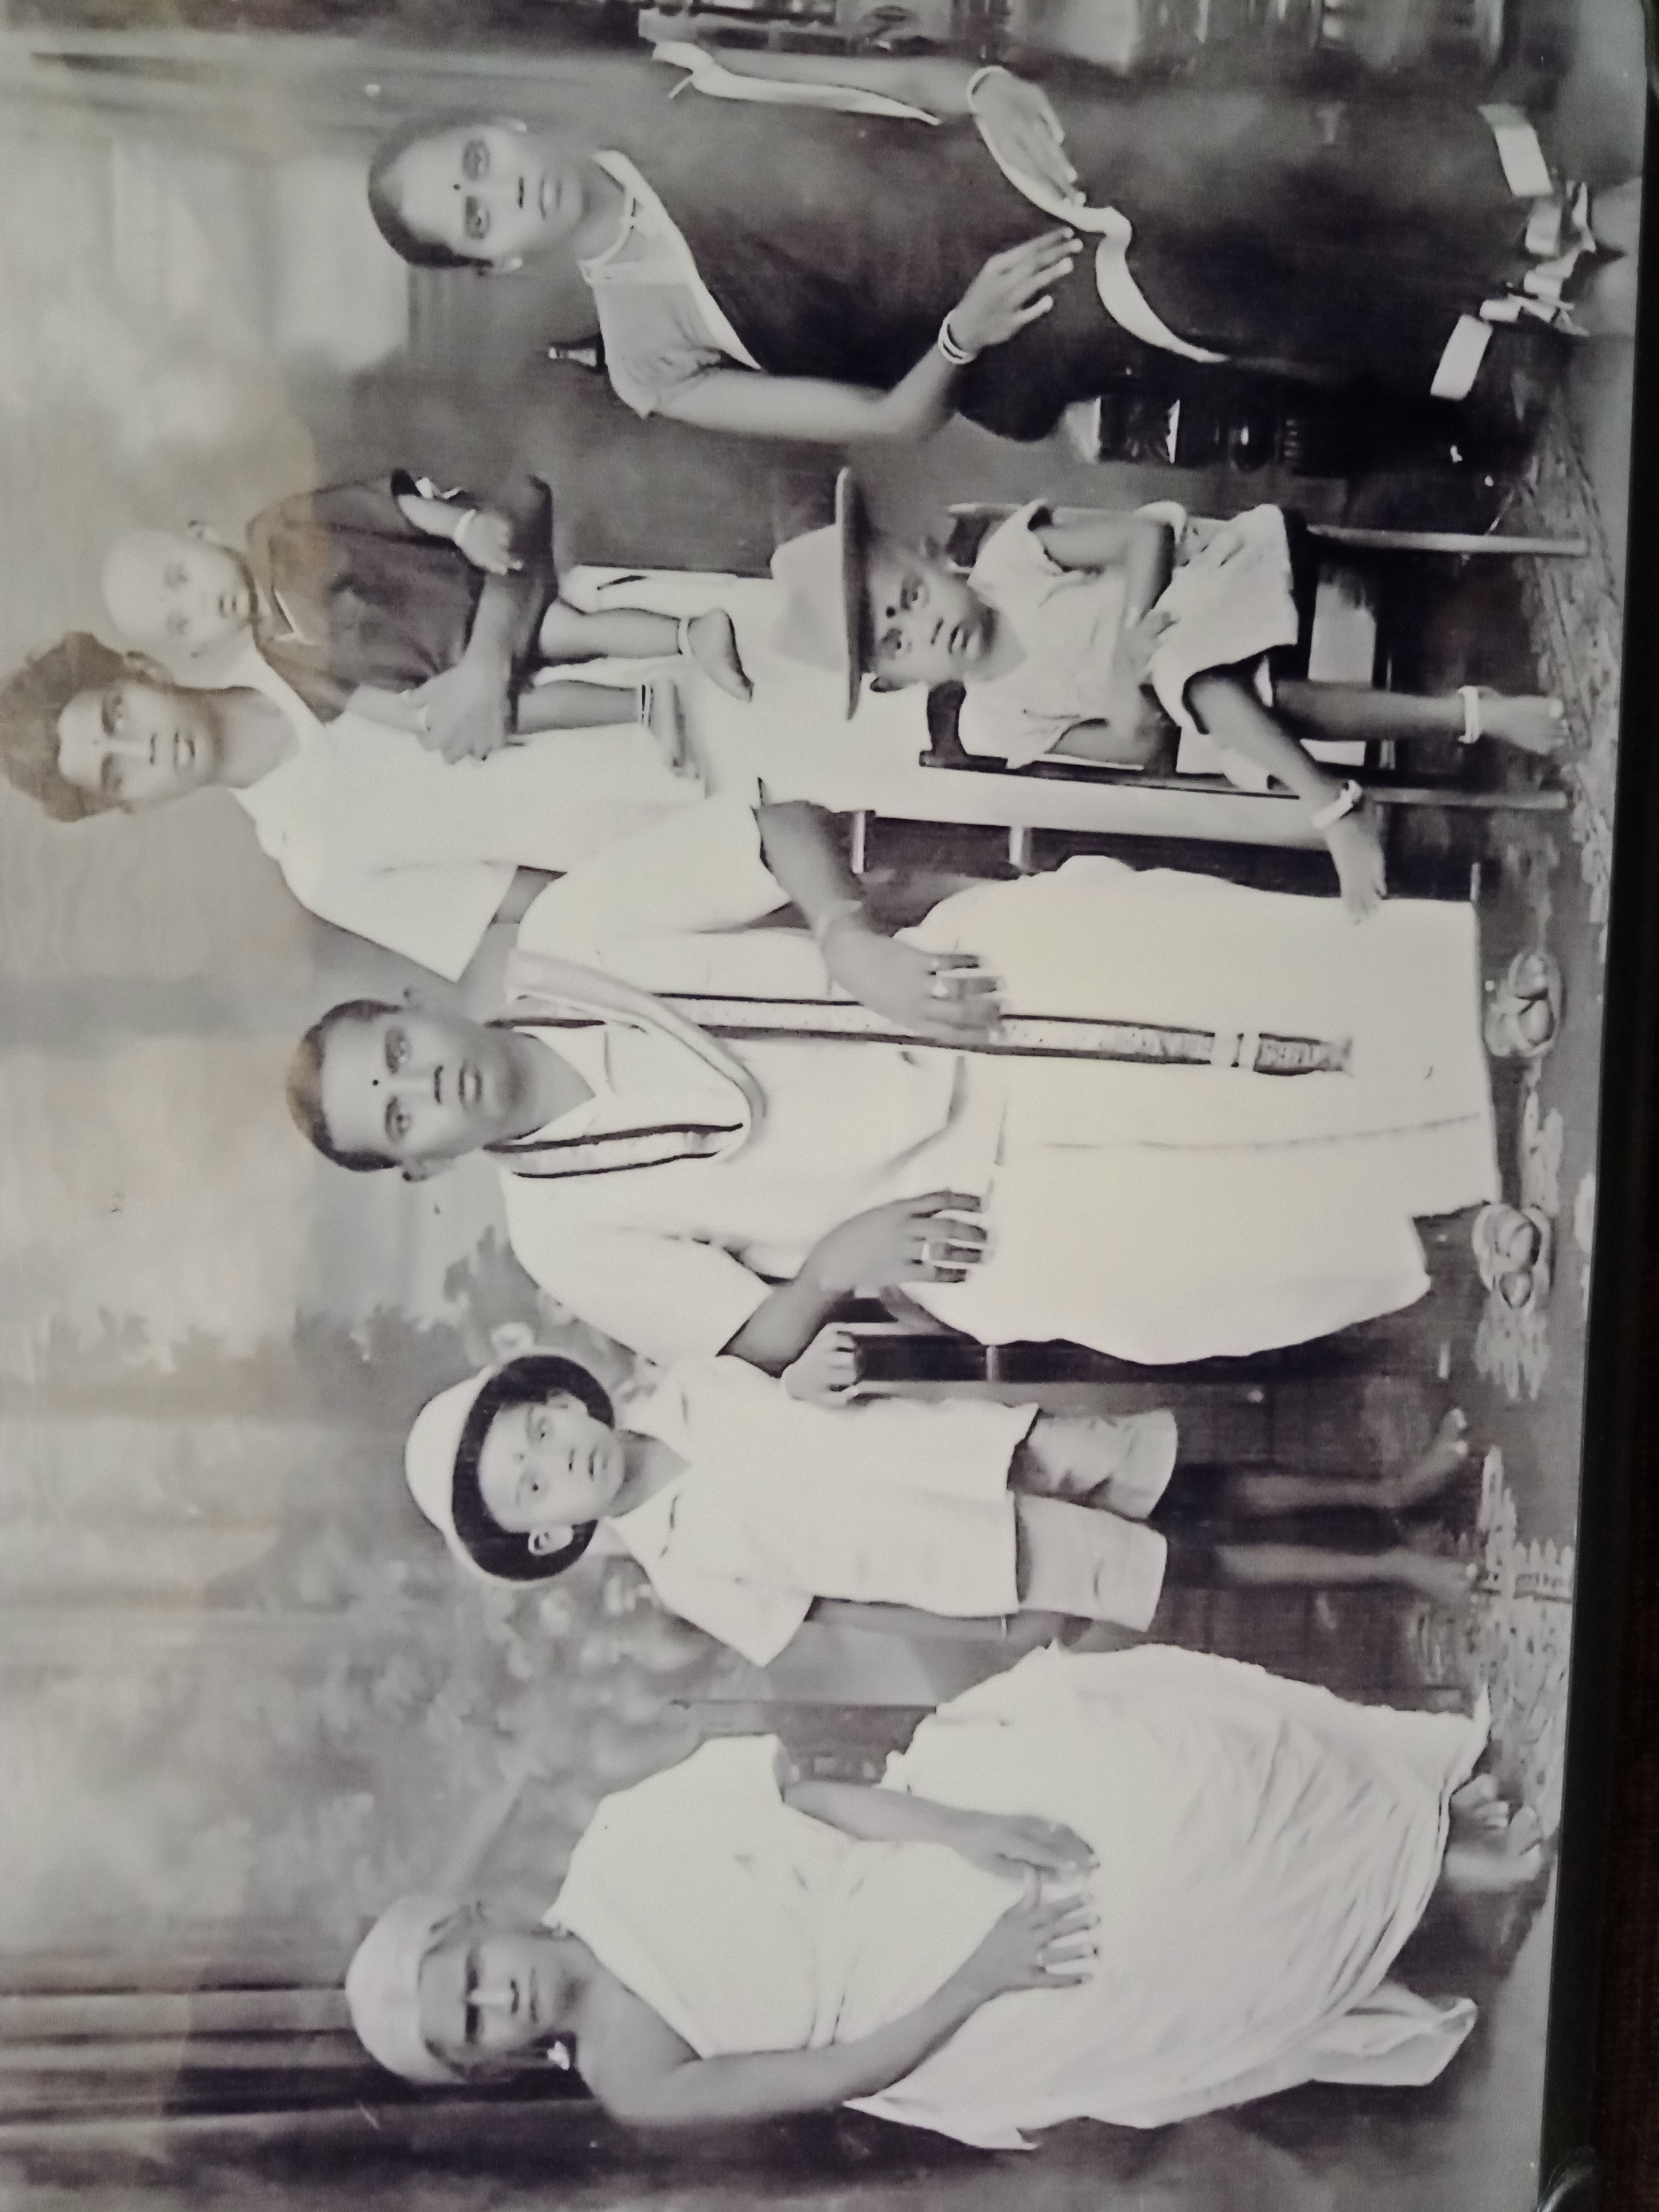
\includegraphics[angle=270,width=0.8\textwidth]{Rajaji-01.jpg}
\caption{Circa 1942. From L to R, My grandmother, GR, my father,
my uncle Ramalingam carrying my brother Rajaguru, my sister
Leelavathi, my mother.}
\end{figure}
My father, VR S S Guruswamy Nadar had a shop selling metal vessels. My 
mother was Ekkimuthammal. I was the first born and had four brothers and 
five sisters, one of the sisters died as an infant.

My father's shop did well and so our family was reasonably well- 
provided, but later my father's earnings in the shop was not enough to 
provide for such a large family.

My father's father, whom I never saw, was Sivagurunatha Nadar. His 
father was perhaps Subramania Nadar and his father was Veerabhadra 
Nadar. So my father's initials start from VR (Veera), then S (Subra), 
and S (Siva). This is how Nadars were generally named. If I were to 
follow this practice, my name would be VR S S G Rajasekara Nadar! 
Although my grand father was not alive when I was born, I was lucky to 
see my grandmother. She passed away when I was in the elementary school.

My father's family was not well-to-do. My father studied only up to 
second standard. In fact I heard that the family was so poor that my 
father made whistles out of palm leaves and sold them to children!

He went to Rangoon and worked as a shop assistant. Those days Indians 
went to Burma or Malaya just as now they go to USA or Middle East. After 
earning enough money he returned and got his three sisters married off. 
Then he married my mother in 1934. As I already said, he did very well 
through the vessel shop.

My mother's father was MR Perumal Nadar. He went to Penang in Malaya and 
did very well. He owned his own shop there. He took my mother to Penang 
for some time. So both my father and mother are foreign-returned!

As ill luck would have it, during the Japanese occupation at the time of 
the Second World War, my grand father had to convert all his money into 
Japanese currency which became worthless after the war. He brought all 
these currency notes and distributed them among children; we used to 
play with them!

But his return to India was an interesting story. For many years during 
the war we did not have any contact with him. It was even thought that 
he was dead. I remember I was persuaded to write a nice letter to him by 
my uncle Ramalingam (my mother's younger brother) for which of course 
there was no reply.

Around the year 1947, my father wanted to take our whole family on a 
pilgrimage to a small town called Yeral. We were waiting for our bus at 
the bus stand. Imagine our surprise, when Perumal Nadar got down from 
the bus!

Perumal Nadar was a very interesting personality. He used to take me to 
the river-side for long walks and advised me to pluck the herbs there 
and eat them. He was also philosophically oriented and gave me many 
books to read.

In my younger days my uncle Ramalingam who was looking after our shop 
took care of me also, like taking me to the well (called Nandavanam) for 
bath, when my father was not there. In fact most of the time I was with 
him in the shop.

There were two deaths which affected me very much in my childhood. My 
baby sister Kanthimathi and my aunt (Ramalingam's young wife). The 
latter died while giving birth to her first son. She was very fond of 
me.

I had three aunts (my father's sisters) Mookkammal, Thenammal and 
Sornammal who lived in another small village, Kokkarankottai. Thenammal 
lived in Aruppukkottai, another town. Mookkammal lived in Kamuthi. Her 
husband died before I was born. She liked me very much and I visited her 
small hut often. She was very poor, but always gave me something to eat. 
Once she could give me only rice mixed with brinjal cooked in oil. It 
was so tasty that even now I like brinjal cooked that way. My father's 
elder brother Rangaswamy Nadar had a vessel shop in a neighboring town 
Abiramam, but did not do well.

There was a Sankara Mutt in Kamuthi. A few Nadars and maybe some from 
other communities belonged to the Mutt. My aunt Mookkammal also belonged 
to it. They were all vegetarians. Once a year there was a pooja and 
meals were served. My aunt took me there.

Another person I liked was my maternal grand mother's sister Meenammal. 
Tragically she had lost her husband and son some time ago. She liked me 
very much and as a child I remember to have spent much time with her in 
her humble hut. She was very poor and eked out a living by selling the 
milk from one or two buffaloes that she kept. She used to carry me on 
her rounds selling the milk.

Meenammal used to go for groundnut-picking in the fields north of 
Kamuthi and she often took me there. The plants had been plucked along 
with the roots. We had to pluck the groundnuts from the roots. At the 
end of the day, one-sixth of what we plucked was our wage. We used to 
roast some of the groundnuts on open fire there itself and they were 
very tasty to eat. My father would not allow me to go, so I went only 
when he was away in Madurai!"

My father along with another Nadar ran a Cinema Theater. I still 
remember my father taking me on the back seat of a bicycle to watch the 
films. But I heard that my father lost a lot of money since the other 
person cheated him. I also heard that the only film that ran well and so 
earned some money for him was ``Rajasekaran" and that is why my father 
named me that!

The very first film that I understood was Nandakumar. My uncle 
Ramalingam took me for it. TR Mahalingam acted as young Krishna and I 
liked it. Another film that I liked and still remember is Laila Majnu. 
There were two versions: one with Nageswara Rao and Bhanumathi with 
Gantasala's songs and the other with TR Mahalingam. Much later when I 
was in American College, Madurai, I saw Devadas (with Nageswara Rao and 
Savitri) and I liked it very much.

The other films that I liked were
Bhaktha Meera (MS Subbulakshmi),
Shakunthalai (MSS),
Savitri (MSS),
Sivakavi (MK Thiagaraja Bhagavathar),
Thiruneelakandar (MKT),
Haridas (MKT),
Chakradhari (V Nagiah).
The other singing stars that I liked were PU Cinnappa, TR Mahalingam and
KB Sundarambal.

There was not much industry in Kamuthi. But I can mention a few things 
of interest. RM T S Soundara Pandian's family was well-to-do among the 
Nadar families and they had earned their money by leather business from 
the time of RM T S S's father Senthilkumar Nadar. They bought the skins 
of the slaughtered goats, treated them and after further treatment in 
their factories in Dindigul and Trichy, sold them. Some were even 
exported abroad.

RM T S S was an important Congress leader in the district and knew 
Kamaraj who visited Kamuthi a few times. He was elected as the President 
of the Panchayat Board. My wife is his daughter. He named her Suthandra 
Devi (Goddess of Liberty) since she was born just after India got 
independance. He passed away during the election propaganda when he was 
talking in support of the Congress candidate.

Another prosperous family in Kamuthi was the family of PNSP Palanichamy 
Nadar who made their money by making snuff from tobacco. Their firm was 
known as Chokkan Palani Vilas. Their shop was adjacent to ours and 
Periaswamy, the eldest son of Palanichamy Nadar, liked me and my family 
had good relations with him. He was many years older than me.

My father brought brass sheets from factories and through the metal 
workers called ``kannars" in Tamil and who lived in Kannarpatti in the 
northwestern part of Kamuthi made vessels which were then sold. This was 
essentially a cottage industry and could have grown up to factory level, 
but didn't.

Opposite our vessel shop was what was called ``kittangikkadai". Kittangi 
is godown and it was used to store rice in gunny bags. It belonged to SS 
Ponnuswamy Nadar whose shop and house also were right there. His son 
Ramasamy was a friend to me and Ramasamy's cousin Rajarathinam (alias 
Jeyaraja)) also was my friend.

A little distance from the southern edge of Kamuthi, recently Adani and 
Co set up what was claimed to be the world's largest solar power plant. 
They got the lands cheaply since they were fallow lands. However this 
has not yet contributed to the industrial development of the region.

One thing that stands out in my memory of those childhood days was our 
visit to Madurai and the Meenakshi temple. On the way to Thirumangalam 
to worship our family deity there, we used to stop at Madurai. In 
addition my father used to take me some times to Madurai. He went to 
Madurai periodically to buy the vessels to be sold at his shop in 
Kamuthi. I always enjoyed these trips. The majestic sky-high gopurams 
and the gigantic temple where every corner had a historical or 
mythological story to tell. The temple was surrounded by roads forming a 
series of concentric roads forming squares, each named after a Tamil 
month. The Old Madurai City was so well planned. My father knew so much 
about the City and the Temple which he conveyed to me. I decided that 
when I grow up I will live in Madurai!

In the beginning we lived in Ramalingam's house. Sometime in the 45-47 
period we moved into a very big house which my father took on lease. It 
had two storeys, many rooms and terraces. Third storey was a open 
terrace and from there we could see the fort at Kottaimedu, since our 
house was the tallest building in the whole area.

The house had a backyard where we had a cow. We children were afraid of 
going to the backside of the house since it was dark and we did not have 
electricity. Cobras were suspected to be around. A snake charmer was 
called and he caught one cobra from inside one of the rooms at the back 
and one in front of the house where there was an empty space. Some 
people said the snake charmer brought his own cobras and pretended to 
catch them!

One night my father was bitten by a small snake in our terrace upstairs, 
but probably it was a non-poisonous snake.

But there were many scorpions and I was stung by them a few times. 
Although it was intense pain, it lasted only twenty four hours! Those 
days, children used to suffer from many diseases such as cholera and 
small-pox. Infact, every year in a particuar season many children died 
of cholera. 

There was one ailment that affected me during every season. 
Every morning when I woke up, the eyes were covered by some discharge 
and it was very painful to wash them. There was a remedy called 
"kaduvudan" which, I think, were the seeds of some plants and these were 
powdered and put into the eyes. It was always done just after midnight 
and operation was always performed by some old ladies (my relatives). It 
was extremely painful, but in the morning, eyes became clear 
miraculously and the ailment was cured.

All these diseases and ailments have disappeared, thanks to advances in 
medical science and better hygiene.
 
Those days the shops remained open even on Sundays. Then the Government 
passed an order that all shops must be closed on Sundays. So every 
Sunday my uncle Ramalingam and a few of his friends (which included 
Periaswamy) used to make poories in the terrace upstairs and it was a 
very enjoyable occasion. Poories were a novelty at that time. In fact 
wheat itself was unknown. During the war rice became scarce and 
government introduced wheat into Tamil Nadu.

Another joyous occasion was full-moon days when my mother along with a 
few neighbours used to cook special meals (called koottanchoru) in the 
terrace. All this happened when we were living in my uncle's house.
 
Once I traveled with my brother Rajaguru by bullock cart to a 
neighboring village called Kollangulam. There Nadar community had landed 
property along with a farm-house. My grandfather was working there as 
the man-in-charge. He had invited us there. We spent a whole day and 
night. Recently, after more than 70 years I visited Kollangulam with 
Rajaguru.

The Nadar community earned quite a bit of money from the land and the 
Muthumariamman Temple was managed with those funds. The community had a 
local government called ``uravin murai" which even levied tax called 
``mahamai"from every Nadar family.

The first educated Nadar from Kamuthi was Dr M Natarajan who was the son 
of Mahalingamurthy Nadar who was a formidable character. People have 
seen him beating his son with the stick part of a palm-leaf fan. Once a 
widow was punished by the uravin murai for crossing into the forbidden 
muslim street. He fought against that and the uravin murai decreed he 
should apologize by symbolically breaking a coconut in front of the 
deity in the temple. He refused to apologize and the uravin murai 
expelled him from the community. He left Kamuthi and thereafter lived in 
Madurai.

After getting MBBS, Natarajan served in the war effort. He went to Japan 
and treated the wounded British and Indian military men. So he was 
awarded a high military rank. After the war, he settled in Madras and 
became a famous orthopedic surgeon. He rose to become the Principal of 
the Madras Medical College.

Natarajan is a relative of my wife and a distant relative of mine. My 
father used to say that if one wants to get educated he should take 
Natarajan as his model.

Kamuthi was an important market-town for the surrounding villages. Every 
Tuesday Kamuthi became a Sandhai (market). People from the surrounding 
areas came on that day and bought or sold things. This activity took 
place mainly in a special area called Sandhai, located in the southern 
part of Kamuthi. The whole town was full of people on that day. There 
was very brisk business in all the shops including our vessel shop.

\section*{School (1941 to 1952)}
I studied in Kshatriya Nadar Higher Elementary School up to the fourth
standard and in Board High School from fourth to the eleventh standard
which is the end point of school education those days.

Among my teachers in the elementary school, I still remember Ulaganatha
Iyer, Subramania Iyer, Subramania Pillai and Alagu Ramaswamy Pillai who
was an excellent teacher.

During the school days, I spent all my time after school, at our shop. 
In fact in my father's absence I have sold many vessels. But my heart was 
not in this business. Since the vessel shop was not busy most of the 
time, I could concentrate on my studies. I came out first usually in 
most subjects.

Apart from the shop, there were two other places which I frequented. One 
was Muthumariamman Temple and the other was Nadar Vidhyabiviruthy Sangam 
which was a library. There were newspapers and monthly magazines. There 
were old books too. Among them I found a book of science where Thomson's 
atomic model was described. It also contained Michael Faraday's 
discovery of electromagnetic induction with excerpts from his diary. I 
enjoyed reading them and it created in me an interest in experimental 
science.

The Sangam was under the care of V Saravana Nadar who was a distant 
relative of mine. He was a bachelor and lived in the Sangam premises.He 
cleaned up the premises and took care of the reading room and the 
library. There was a radio upstairs that was also under his control. 
News by All India Radio and good carnatic music emanated from the horn 
loudspeaker. We got the news about Gandhiji's assassination on 30 
January 1948 from this radio. Our house was a little distant from the 
Sangam, but the direction of the loudspeaker was such that I could hear 
the music sitting on our upstairs window, especially in the nights. 
This was my first encounter with beautiful carnatic music!

Now a guest house with AC rooms and attached bathrooms has been added to 
Sangam and I stay there during my visits to Kamuthi.

I was very much attracted by the Muthumariamman Temple which was close 
to my home. I liked to watch the priest doing pooja to the deity and 
went with the deity in all the temple processions during the festivals.
  
In 1945 Germany was defeated in the II World War and it was celebrated 
in India which was under the British rule at that time. So the Union 
Jack was flying over the Tahsildar's office. After a while it was 
removed. I asked my father why was it removed. Like most children I 
liked the colourful flag. My father said in any case it was not our 
flag, we were being ruled by the British. That is the first time I 
became aware that we were not independent.

When I studied there, the Kshatriya Nadar Higher Elementary School had 
only up to eighth standard. It started maybe a century earlier. Later, 
after my time there, this school became a High School with classes up to 
twelve. Although it has the Nadar name, it caters to all the castes. 
In fact now most of the students are from the surrounding villages and 
students from other castes, especially Thevars. Hence 
the School administered by the Nadars has been doing good social 
service.

A few years ago, the Nadar School celebrated the Golden Jubilee of its 
High School version and I attended it.

At school a Muslim boy was saying Gandhi was sent to the jail. I asked 
who was Gandhi. He said he was Jinnah's opponent. That was the first 
time I heard of Gandhi.

Maybe it was 1946. There was news that Gandhiji was coming to Madurai. 
My father planned to go to Madurai to see Gandhiji. I requested him to 
take me with him and he agreed. But unfortunately, my father could not 
go for some reason and I lost my only opportunity to see Gandhiji.

Actually, it was neither Gandhiji nor Nehru but Netaji Subhash Chandra 
Bose who was popular among the youngsters. All of us carried a photo of 
Bose in military uniform in our pockets in defiance of the British 
Government who considered that as a punishable offense.

Independence came in 1947 and on that day I was not in Kamuthi. My 
father took all of us to Yeral, a pilgrimage town, the same trip which 
was postponed due to the arrival of my grandfather. We were all sleeping 
in the Chathiram of the temple on the night of 14 August 1947. We were 
woken up at midnight because they wanted to clean up the Chathiram on 
the eve of the Independence Day. Next morning Lord Subramanya during the 
procession was wearing a garland made of charka-spun threads. That is 
how we celebrated Independence of India.

Since I was a top student in the elementary school, my father's friends 
advised him to shift me to the High School after I finished class four. 
When my father took me from the elementary school to put me in the high 
school, it was Chellappandian, the class five teacher in the high school 
who took charge of me. He asked me to write an essay on ``The Cow" in 
English. Since Alagu Ramaswamy Pillai at the Elementary School had 
taught me English, I could write `` The cow has four legs and one 
tail....". Chellappandian admitted me into class five.

Apart from Chellappandian, I had many excellent teachers in the high 
school - Edward Muthuswamy Pillai, Chellam Pillai, Karuppaswamy 
Thevar... and above all Subramania Iyer, the Head Master and English 
teacher for class eleven (which was called sixth form). The way he 
taught Shakespeare is still ringing in my ears! He trained me to act as 
Mark Antony in the Annual Day of the School and my rendering of Antony's 
peroration after Julius Ceaser's assassination was a great success! The 
local doctor Thirunavukkarasu recalled it whenever he saw me and 
congratulated me.

There was a custom of putting up the day's news in a black board at the 
morning's prayer meeting at the school. Following the Headmaster's 
command, I chose the headlines from The HINDU every day and put it up. 
This also gave me good practice in the English language.

There is one incident I cannot forget. In class eight (third form) there 
were two sections taught by Edward and Chellam Pillai. Since Edward had 
impressed me very much as a good and interesting teacher in the second 
form, I wanted to go to the section of Edward. But I was put in the 
other section. They did not allow me to change the section since that 
was apparently against the rules. I was very disappointed.

But what happened afterwards proved to be an anticlimax! Chellam Pillai 
turned out to be an excellent teacher. Not only that. Since I was the 
first in the class and especially because he liked me, he made me the 
monitor and put the whole class under me. In the class tests, I was 
asked to invigilate with powers to punish the wrong-doers!

We were taught Tamil by two Tamil Pandits, Koormavatara Konar and then 
Heramba Iyer. Both could compose Tamil poems on the spot. In fact the 
latter when he scolded the students, it was in the form of a poem!

Hindi was taught in the high school, but then the Hindi agitation by DMK 
caused the abolition of Hindi teaching. The Hindi Pandit Nagarajan lost 
his job. A few of us who wanted to learn Hindi paid Nagarajan and he 
taught us. He was a very good teacher and I passed the Prathamic, 
Madhyama and Praveshika examinations conducted by the Dakshina Bharatha 
Hindi Prachar Sabha. I do not remember whether I went for the Rashtra 
Bhasha examination also.

Karuppaswamy Thevar was our manual training (carpentry) teacher. But 
apart from that he taught us Thirukkural since he was a great admirer of 
Thiruvalluvar. He was also a staunch advocate of vegetarianism, but more 
on that later.
 
A big problem with the high school was the absence of good teachers for 
science. Since Kamuthi was a backward area, even the teachers who joined 
left soon. We did not have a teacher for Maths. As a result my school 
abandoned Algebra and Geometry and only Arithmetic was taught. Algebra 
and Geometry were called Composite Mathematics and it was not done. So 
when I go to College I would not be eligible for First Group 
(Mathematics, Physics and Chemistry). But my good Headmaster advised my 
father to buy the standard text books on Algebra and Geometry and 
advised me to learn them by myself. This is how I spent my vacations.

So my knowledge of Mathematics had many gaps. In spite of that I got 
first group in the College.

The High School was situated at the southern end of the town. It was 
just thatched sheds. When I had completed the High School, it shifted to 
pukka buildings to the north of the town, at Kottaimedu. The Chief 
Minister inaugurated it. It continued for many years, but now I hear it 
has been converted into a College!

When I was in Kamuthi recently, I had a surprise. I went with my brother 
Krishnamoorthy to the location where my old school in thatched shed was 
situated. It was still there! Actually after the Board High School 
shifted to Kottaimedu, the shed housed a Muslim School. That also 
shifted and they were going to demolish the shed, but they had not done 
it when I visited. So I was very lucky to see my old school!

We had a cow at home. The cow and its calf were sent outside the town 
for grazing every day. One day the cow alone returned. It was noticed 
fairly late in the night. My father and myself went with a torch and we 
could locate the poor calf which was huddling against a wall. Every one 
was happy to see the calf.

Another time, I lost my gold ring while playing football in the high 
school. Again it was noticed only late in the night. My father and 
myself went to the football ground in the high school. Even though the 
football field was very big, I managed to find the ring!

There was no electrical connection at our home, but the shop had it. So 
not only myself, but all my brothers and sisters also studied in the 
evenings at my shop. But my studies continued even after the shop was 
closed, especially during the exam period. So I used to study in the 
light of a kerosene lamp sitting in the bed. Once I fell asleep and the 
open kerosene lamp fell. A serious accident was averted only because my 
parents noticed it in time. After that I was forbidden to study in the 
bed.
 
I passed out the government examination, called SSLC (Secondary School 
Leaving Certificate) exam, with good marks and went to study 
Intermediate in The American College in 1952. This was a big step in our 
family. By that time our shop was not doing well and my father needed me 
to help him. My uncle who was helping him in the shop left him and 
started his own vessels shop which was a rival to our shop. My mother 
did not like my going away. But my father wanted me to pursue higher 
education. His idea of higher education was either to go for the IAS 
examination or start a big business with the help of my education.

Where can the money for my higher education come from? Clearly my father 
could not afford it. I got a loan scholarship from Nadar Mahajana Sangam 
which had to be repaid. I also got a merit-cum-means aid from the Madras 
Government. None of this was enough since the hostel expenses were high. 
My father had to take it from our shop which went down further as a 
consequence. Later I could compensate him but that was much later. Even 
from my Training School stipend of Rs 150, I could send him a large part 
of it. I continued to do it from my TIFR salary. Since TIFR continued to 
pay my research assistant salary when they sent me to Chicago I sent him 
the whole of it. Not only that. I saved a large part of my assistantship 
money in Chicago and sent it. As a consequence he could build a new 
house. Until then we did not own a house.

One reason our shop did not do well was this: my father bought some land 
and he could not concentrate on the shop. From land also he did not get 
any income since we were in a rain-deficient region.

Among my brothers only one, G Krishnamoorthy could rise high in 
education. He became a Professor in TIFR. He was financially supported 
by me after I began to earn. Another, Arunachalam also was supported by 
me and he got employed in a bank. The oldest of my brothers, Rajaguru 
became a successful businessman. He along with his three sons became 
manufacturers and traders of furniture at Madras. Ramachandran did not 
study well and never did anything. He died some time ago. Among my 
sisters none completed school education although two of them did very 
well in elementary school. Unfortunately, my mother stood against their 
education and even my father could not do anything.

Actually after my father's time I wanted that our house and other landed 
property must go to my sisters only since none of them was well-to-do.  
My mother and brothers did not agree and did not want any part of it to 
go to my sisters. I did not want to take any part of it although the 
house was built solely from my money. I cut off all connection with all 
of them and Kamuthi. After many years, all this has been forgotten and 
now I have good relationship with all of them. I went back to Kamuthi 
only after 40 years!
 
\section*{The American College, Madurai (1952 to 1954)}

Intermediate was roughly equivalent to the present plus two. In spite of 
some gaps in my Mathematics, I was admitted to the first group 
consisting of Maths, Physics and Chemistry.

American College was an exhilarating experience for me. The stately 
buildings and the excellent faculty of the college impressed me very 
much. I stayed in the Wallace Hall which was one of the three hostels. 
ES Moses taught me physics and Ramaswamy taught me chemistry. I have 
preserved the excellent notes of Ramaswamy's lectures that I took. T 
Natarajan, Benjamin Gunaraj, Gift Siromoney and a few other very good 
teachers taught mathematics.

I had two very good friends in the college. K S Ramakrishnan who went 
for IAS and later resigned because of his honesty. I have very good 
contact with him. The other, M Pathamuthu became a Gandhian and lives in 
a village near Madurai.

It may be 1953 or 54, Nehru visited Madurai. I had come home on 
vacation. I wanted to see Nehru. My father permitted me to go. The whole 
temple city was decorated to welcome Nehru. He was supposed to pass 
through the road in front of American College. My friend Pathamuthu and 
myself stationed ourselves at a vantage point inside the college campus. 
When Nehru's car came near the college, a group of DMK fellows threw 
something at Nehru's face. It was stones inside a black cloth. For a 
moment Nehru's face showed his pain but his smiling face appeared soon. 
I hated this barbaric act by some of the MCC students.

During one weekend, myself and a few friends (Pathamuthu, Sakthivel and 
Solaivasaham) went on a trip to the Alagar Koil which was in a 
neighboring hill to the north of Madurai. It was a nice picnic.

Alagar Koil is a famous temple for Lord Vishnu (Alagar). During the 
Chithirai festival of the Meenakshi Temple, Alagar comes down to 
Madurai and in the early morning enters into the river Vaigai. Lakhs of 
people come to witness this event.

During a recent visit to Madurai, I was lucky to witness this event of 
Alagar entering Vaigai.

It is said that Alagar, that is Vishnu, being the elder brother of 
Meenakshi, was coming down to give her away in marriage to Lord Shiva. 
But Vaigai was in floods and he was delayed. The marriage was held 
without him and Alagar returned to his abode in anger.
 
There was religious instruction for Christians and moral instruction for 
others. My moral instruction class was taken by an Economics Professor 
KJ Charles. His lectures were fantastic. He lectured on Marcus Aurelius, 
Thomas Aquinas and Albert Einstein. I learnt about Einstein in a moral 
instruction class!

But I had heard Einsteins's name from my Tamil Text book in the high 
school. Mu Varadarasanar's article mentioned the famous lines of Kaniyan 
Poongunranar in a Purananuru poem
          ``Yathum ooray,yavarum kelir"
(All places are mine and all are my relatives).
and called the poet the Einstein of social sciences!   

A crucial event occurred during the American College period. A friend 
took me to watch the night sky from the terrace of the Mathematics 
building. It is a look through the College telescope that determined my 
trajectory in this life.

It just happened that it was the best time to observe the Moon. When it 
is dark of course you cannot view it and when it is fully bright it does 
not show its features clearly. But that day was the half-way point 
between New Moon and Full Moon days. The shadows cast by the mountains 
in the Moon got elongated, with sharp edges. I felt as if I was standing 
on an elevated height above the Moon, looking down. It was so 
frightening, the mountains and craters. It was a fantastic experience. I 
realized

``There were more things in Heaven and Earth than were dreamt of in my 
philosophy".

Since Science alone held the key to these other ``things" I had no 
hesitation in my choice of what I wanted to do. I am sure many others 
too have been lured into Science through Astronomy.

I went to the Daniel Poor Library (It was not a poor library at all! 
Poor was the name of the donor of the library in the College. It was a 
well-provided library.) and borrowed many interesting books. Eddington's 
(or is it James Jeans) ``Expanding Universe", George Gamow's ``Life and 
death of the Sun" are some of the books that I read and enjoyed. My 
interest in Astronomy and Physics increased further. I published my 
first article ``The Mysterious Universe" in the College magazine.

At the end of my intermediate in 1954, it was clear to me what I should 
do. I must pursue Physics. In those days Madras University had a 
programme for keen students called Honours. But it was offered in very 
few colleges and it was tough to get in. My father of course agreed, 
in spite of my mother's objections.

\section*{Madras Christian College (1954 to 1957)}

B Sc (Hons) in Physics was offered in St Joseph's College, Trichy, 
Madras Christian College and Presidency College. I applied to St, 
Joseph's and Christian. I got admission in St Joseph's. I had secured 
very good marks in the intermediate exam, so I should have got admission 
in Christian College also which is the preferred choice.  There were 
postal delays in getting my marks from Madras to Kamuthi and then from 
Kamuthi to the College. The eleven seats in Christian were already 
filled. So I was offered Maths Hons. But I was told that I can shift to 
Physics if a vacancy arises due to someone leaving for engineering.

I decided to take the chance at Madras Christian College (MCC). I 
attended the Maths Hons class but the lectures were too dull for me. 
Everyday I went to the Principal's office and enquired about the Physics 
seat. The Principal's secretary Ernest will tell me as soon as he saw my 
head at the window ``No". I was getting frustrated. Meanwhile there was 
pressure from my mother to return and look after the shop.

After many weeks, the miracle happened. The secretary told me that Mr 
Kannan has left BSc (Hons) to join Engineering College. I felt Lord 
Krishna (Kannan, in Tamil) Himself came and rescued me!

I got what I wanted and concentrated on Physics. The lectures by PK 
John, SS Thanaraj, CB Rajagopal, KB Rajangam and above all, Dr MA 
Thangaraj were excellent. KB Rajangam taught Bohr's model of the Atom 
and it was so good. I cannot forget them. After that, Thangaraj the Head 
of the Department taught Quantum Mechanics. He used Rojansky's book. 
Those days (1956-57) that was the only book on Quantum Mechanics.

The books that I liked were Modern Physics by Richtmayer and Kennard, 
Heat and Thermodynamics by Saha and Srivastava and Properties of Matter 
by Newman and Searle. The last book had many problems and I enjoyed 
solving them during vacation. They were not mere numerical problems. The 
problem had to be formulated in terms of equations which had to be 
solved.

Thangaraj also taught Wireless and Electronics. That was the only 
subject that I did not like, although that was supposed be the special 
subject in our Hons course. Every other subject was taught as Physics, 
but this was taught more like an engineering subject, just a set of 
prescriptions. Instead of using the standard prescribed text book by 
Terman, he was teaching from the Admiralty Handbook of the British Navy! 
In the Wireless and Electronics exam, I almost failed. Thangaraj was 
also my hostel warden. He called for me in the hostel next morning and 
scolded me thoroughly. For a big question I had answered but had crossed 
it out. He said it was a correct answer and I should not have cancelled 
it. But he passed me nevertheless!

During 1956-57 the syllabus changed and MA Thangaraj found that none of 
the faculty could teach according to the new syllabus which was 
considerably advanced. He assigned the tutor TN Seshan to teach all the 
subjects to us in the final year of the course. Seshan did a marvelous 
job. Later he passed the IAS exam with first rank and became a very 
famous (but not popular) administrator. The high point of his career was 
as Chief Election Commissioner when he reformed the whole election 
process in India.

On weak ends I traveled from Tambaram to Thiruvallikkeni and went to 
the University Library. Among the things that I read there were the 
original papers of Rutherford discovering the atomic nucleus through 
scattering by alpha particles and Niels Bohr proposing his model of the 
atom. It was a special fascination to read these classic papers.
 
The specialty of the MCC (Madras Christian College) situated in 
Tambaram, a suburb of Madras was the Hostel system. There were three 
hostels St Thomas Hall, Bishop Heber Hall and Selaiyur Hall. I belonged 
to St Thomas. Not only the out-of-station students but the so-called 
day-scholars also belonged to one of these halls and developed an 
affinity towards the hall to which the student belonged. Only the 
lectures and laboratories were in the College. All the extra-curricular 
activities were in the halls. I had two classmates who were my friends 
Ratnaprabhu and Mahalingam. Ratnaprabhu became a textile engineer and 
rose to the level of the Director of Ahmadabad Textile Institute and 
Mahalingam became an officer of Indian Airports Authority.

On a Hostel Day, MK Thiagaraja Bhagavathar was invited. He talked and 
sang. I regret that I did not talk to him. For, later I became a fervent 
admirer of his devotional songs. His golden voice captivates me. There 
is none like him.

While at MCC we had to attend intercollegiate lectures at Presidency 
College and Alagappa College of Technology. Two series of lectures were 
memorable. One was by G N Ramachandran who lectured on General Theory of 
Relativity(GTR) although I was still not academically mature enough to 
understand GTR fully. The other was by Alladi Ramakrishnan who lectured 
on the Matrix version of Quantum Mechanics which had not been taught at 
MCC. He was such a powerful lecturer that I was impressed very much.

Here also there were moral instruction classes; they were taken by 
Kibble, a Professor of Mathematics. He used to let us do anything 
quietly when he was looking at his book! There is a good story about his 
absent- mindedness. One day he wanted to go to the city and boarded the 
electric train. He took his book and began to read. After a few hours he 
noticed that he was still in Tambaram station. He accosted a railway 
official and asked him why the train did not leave after so many hours. 
The official said `` Professor, the train has made two trips to Beach 
station!". That was Professor Kibble.
 
His son is the famous theoretical physicist TWB Kibble who was born in 
Tambaram and spent his childhood in the MCC campus. He is the author of 
the nonabelian version of the famous Higgs mechanism. Later during the 
Golden Jubilee celebration of IMSc, I invited him to the Institute and 
took him to MCC where he enjoyed seeing the places of his childhood 
days. He could even identify the tree which he used to climb!
  
I was staying at St Thomas with Villimadan, also from Kamuthi, one year 
senior to me. One day Karuppaswamy Thevar, our teacher from Kamuthi 
visited us. We hid the fact that we ate at the non-vegetarian mess and 
took him to the veg mess. The fact that I had to hide the truth from my 
teacher affected me very much.

Apart from the above, there were other things. At home everybody was a 
non-veg. Since I was the eldest son, I was sent to buy meat. I had to go 
every Wednesday to the slaughter-house. One day I witnessed a goat being 
slaughtered. I saw my mother putting live fish (ayirai meen) into 
boiling water. Every Deepavali day in the early morning my mother would 
cut the neck of our pet hen which was screeching. All these events, 
along with the teachings of Buddha, Gandhi and Thiruvalluvar made me to 
take the following step.

I shifted to the veg mess. But when I went home on vacation, my father 
learnt about it and chided me and compelled me to shift back to non-veg 
mess. I had to do it. He said vegetarianism will ruin my health. I 
argued by citing the example of brahmins and others who were 
vegetarians. He would not agree.

So I had to take non-veg food and could become a vegetarian only after I 
went to Bombay and so became free of my father's influence.
 
A tragic event took place in 1956. My friend Villimadan died in the big 
train crash. The Thoothukkudi Express fell down from the bridge at 
Ariyaloor with considerable number of deaths. Villimadan perished in 
that. He was on his way to a job interview. After hearing of this 
accident, the Minister for Railways Lal Bahadur Sastri immediately 
resigned. Such honesty and selflessness has been very rare in Indian 
political circles.

In the year 1956, it was announced that CV Raman was going to lecture at 
the Presidency College. Thangaraj asked us to go and attend the lecture. 
I think he also attended.

Raman lectured on his theory of specific heat based on the discrete 
frequencies of the crystal vibrations and contrasted it with the 
continuum theory of Peter Debye. At one point his voice rose and he said 
``Debye's theory is not worth the paper on which it is written". So 
saying, he threw the sheaves of paper in his hand and they flew over our 
head and fell into the waste basket. We were all very much impressed. 
Bored as we were with many uninspiring lectures in the class rooms, we 
felt this is how lectures must be given!

The examinations were very tough. I had to revise the whole subject and 
keep it in my fingertips, otherwise there was hardly any time to 
complete the paper. So, many times I used to stay awake whole night 
before the exam. Such a thing happened before the Electricity and 
Magnetism paper which was the last one. After the exams I went to 
Kamuthi and there one morning I noticed that my eye-balls did not move. 
For seeing anything which was a little to the right or left, I had to 
move my head! My parents became alarmed and it was decided that next day 
I must be taken to the famous Dr Joseph's eye-hospital at Trichy. Those 
days that was the only place for eye ailments. But miraculously, the 
next day my eyes became completely normal!

While I was in MCC, scientists from TIFR (Tata Institute of Fundamental 
Research, Bombay) conducted many cosmic ray experiments in the College 
grounds. They sent up balloons to the upper atmosphere and recovered the 
instrument package after many hours. The instrument was special 
photographic emulsion that recorded the cosmic ray particle tracks. So I 
had the opportunity to meet many TIFR scientists who visited the College 
and gave lectures. Bernard Peters, MGK Menon, RR Daniel, D Lal, Gokhale, 
G Venkataraman. PJ Lavakare. I decided to pursue research in TIFR.

Thangaraj had a research project on Cosmic Rays. He sent nuclear 
emulsion up by baloon and recovered them after a while. The emulsion 
contained the tracks of particles that he studied with some research 
assistants. To recover the baloon one has to track it during its flight 
and note the direction of its fall. Once a baloon was almost lost and he 
asked his students to search for it. We were lying on our back on the 
terrace of the meteorological observatory of the Meenambakkam airport 
and peering through binoculars. I succeeded in sighting the baloon and 
so later it could be recovered! Everybody including Thangaraj was happy.

\section*{The Training School (1957 to 1958)}

  Homi Bhabha had this great idea of the Training School where he could
  develop the human resources needed for the Atomic Energy Programme
  instead of taking away scientists from the existing scientific establishments
  and universities.   

  It is now called BARC Training School, but the name at that
  time was AEETTS (Atomic Energy Establishment, Trombay, Training School)
  and it was to start in August 1957. So it was just right for me since I
  had completed my Hons degree at that time.

I applied and was called for interview in Bombay. I did the interview 
well, but admission letter did not come. Got frustrated and went to 
American College for interview for the physics lecturer's job. SJ 
Savarirayan was the Principal and Head of the Physics Department. After 
the interview, he asked me to join immediately. I told him that I am 
expecting a call from Department of Atomic Energy Training School. If I 
do not get it, I will come. He was greatly surprised: I am offering you 
a lecturer's post straight after your degree and you want to go to some 
school! He had not heard of Department of Atomic Energy those days! 
Finally I got the letter from Bombay and joined the Training School.

  Bhabha chose Dr Raja Ramanna to be in-charge of the Training School,
  and chose Dr K K Damodaran to be its active head.
  Dr Damodaran organised all the daily activities of the
  School and took good care of all of us. We (the trainees)
  used to refer to him as the ``Headmaster" of the School (among
  ourselves), but he was much more than that, he was almost
  the local guardian for all of us.

  Bhabha had a predilection for appointing military men as
  administrators. Perhaps he felt that only military men could
  control the unruly crowd that we were! He appointed a military
  person Suraj Prakash as our warden. I remember him as a tall
  and handsome young man, but there was some problem and he was
  rather unceremoniously replaced by Colonel Ottley.
  More about the Colonel later.

  Bhabha gave an inspiring lecture on the opening day of the
  Training School. He talked about his dream of bringing
  nuclear energy to this country and told us how he expected
  the trainees to help to realize that dream. But at the end
  of his talk which was aimed at the sky, we were brought
  down to earth by a question from the audience (namely 
  one of my would-be trainee colleagues). He asked what job we
  were going to get, after the training period. Nowadays it
  is common to find that young people are mostly career-minded.
  They want to know what they will get after one year and what
  after 5 years etc. Asking for the so called career-profile
  has become the standard procedure. Fifty years ago that
  was not the done thing. Most of us had our mind on the sky
  and were not practical-minded. That was why we were taken
  aback by the above question from our colleague. But 
  Bhabha answered the question very effectively. He
  said the questioner can take his (Bhabha's) job if he
  proves himself! Bhabha was not bluffing, for a trainee from
  the 6th batch of the School (Dr Anil Kakodkar) became
  the DAE Chief, although Bhabha himself did not live to
  see that.

  Our hostel was at Land's End, Bandra. It was really Land's
  End! The road ended and the sea started. In between the end of
  the road (where there was a band stand) and the sea coast
  full of black rocks characteristic of the Bombay coastline,
  there stood rows of military barracks which had been in use
  during the second world war. Each building had a spartan
  simplicity: four walls mounted by a semi-cylindrical ceiling made of
  corrugated iron sheet. This was partitioned into two rooms
  and each room contained two trainees. This was the Training
  School hostel to be compared to the present sleek
  multi-storey building in Anushakthi Nagar.

  The classes were held in the Churchgate area, either in the
  Jai Hind College or in the K C College. Some classes were
  also held in the new TIFR building that was coming up in
  the Holiday Camp (now called Navy Nagar). In fact I still
  remember cement and bricks falling through one part of
  the TIFR room when the lecture or tutorial was going on.
  So we commuted between Bandra and Churchgate.

The training school teachers came from BARC and TIFR. KK Gupta and 
Viswanathan taught Classical Mechanics. KS Singhwi and Anisur Rahman 
taught Quantum Mechanics, Gaurangh B Yodh taught Electricity and 
Magnetism, Ammiraju and Kondaiah taught Nuclear Physics, Babulal Saraf 
taught Kinetic Theory and Thermodynamics, MGK Menon taught Passage of 
Radiation through Matter, LS Kothari taught Solid State Physics, BM 
Udgaonkar taught Reactor Physics, MR Srinivasan taught Reactor 
Engineering. and George Abraham and R Narasimhan taught Mathematics. 
There were many other subjects like Electronics and Health Physics too. 
It was very impressive. I learnt a lot, much beyond what I learnt in the 
college.

Most of the teachers were excellent. We voted KK Gupta as the best teacher.
In our batch there were 50 + 50 + 50 trainees,in Physics, Chemistry
and Engineering. There were no girls! Over the years, all this has changed.
There were many South Indians among us. We used to come to the hostel 
mess in dhoties. Ramanna passed an order disallowing dhoties. We went on 
a hunger strike. It ended after a day; we capitulated after a day of 
starvation!

I got first rank at the end of the training. For that I received the 
Homi Bhabha Gold medal from Prime Minister Manmohan Singh during the 
Golden Jubilee celebration of the Training School in 2007. But that was 
the second award for the same thing! Since I got not only first rank but 
my marks were way above those of the nearest to me, Colonel Ottley the 
hostel warden gifted me a book: ``The man in the grey flannel suit". It 
was filmed in Hollywood with the famous actor Gregory Peck.
 
I got freedom to choose between TIFR and AEET for my research. All the 
trainees who were above a certain rank were allowed to choose BARC 
(called AEET at that time) or TIFR. I chose TIFR.
\begin{figure*}[h]
\centering
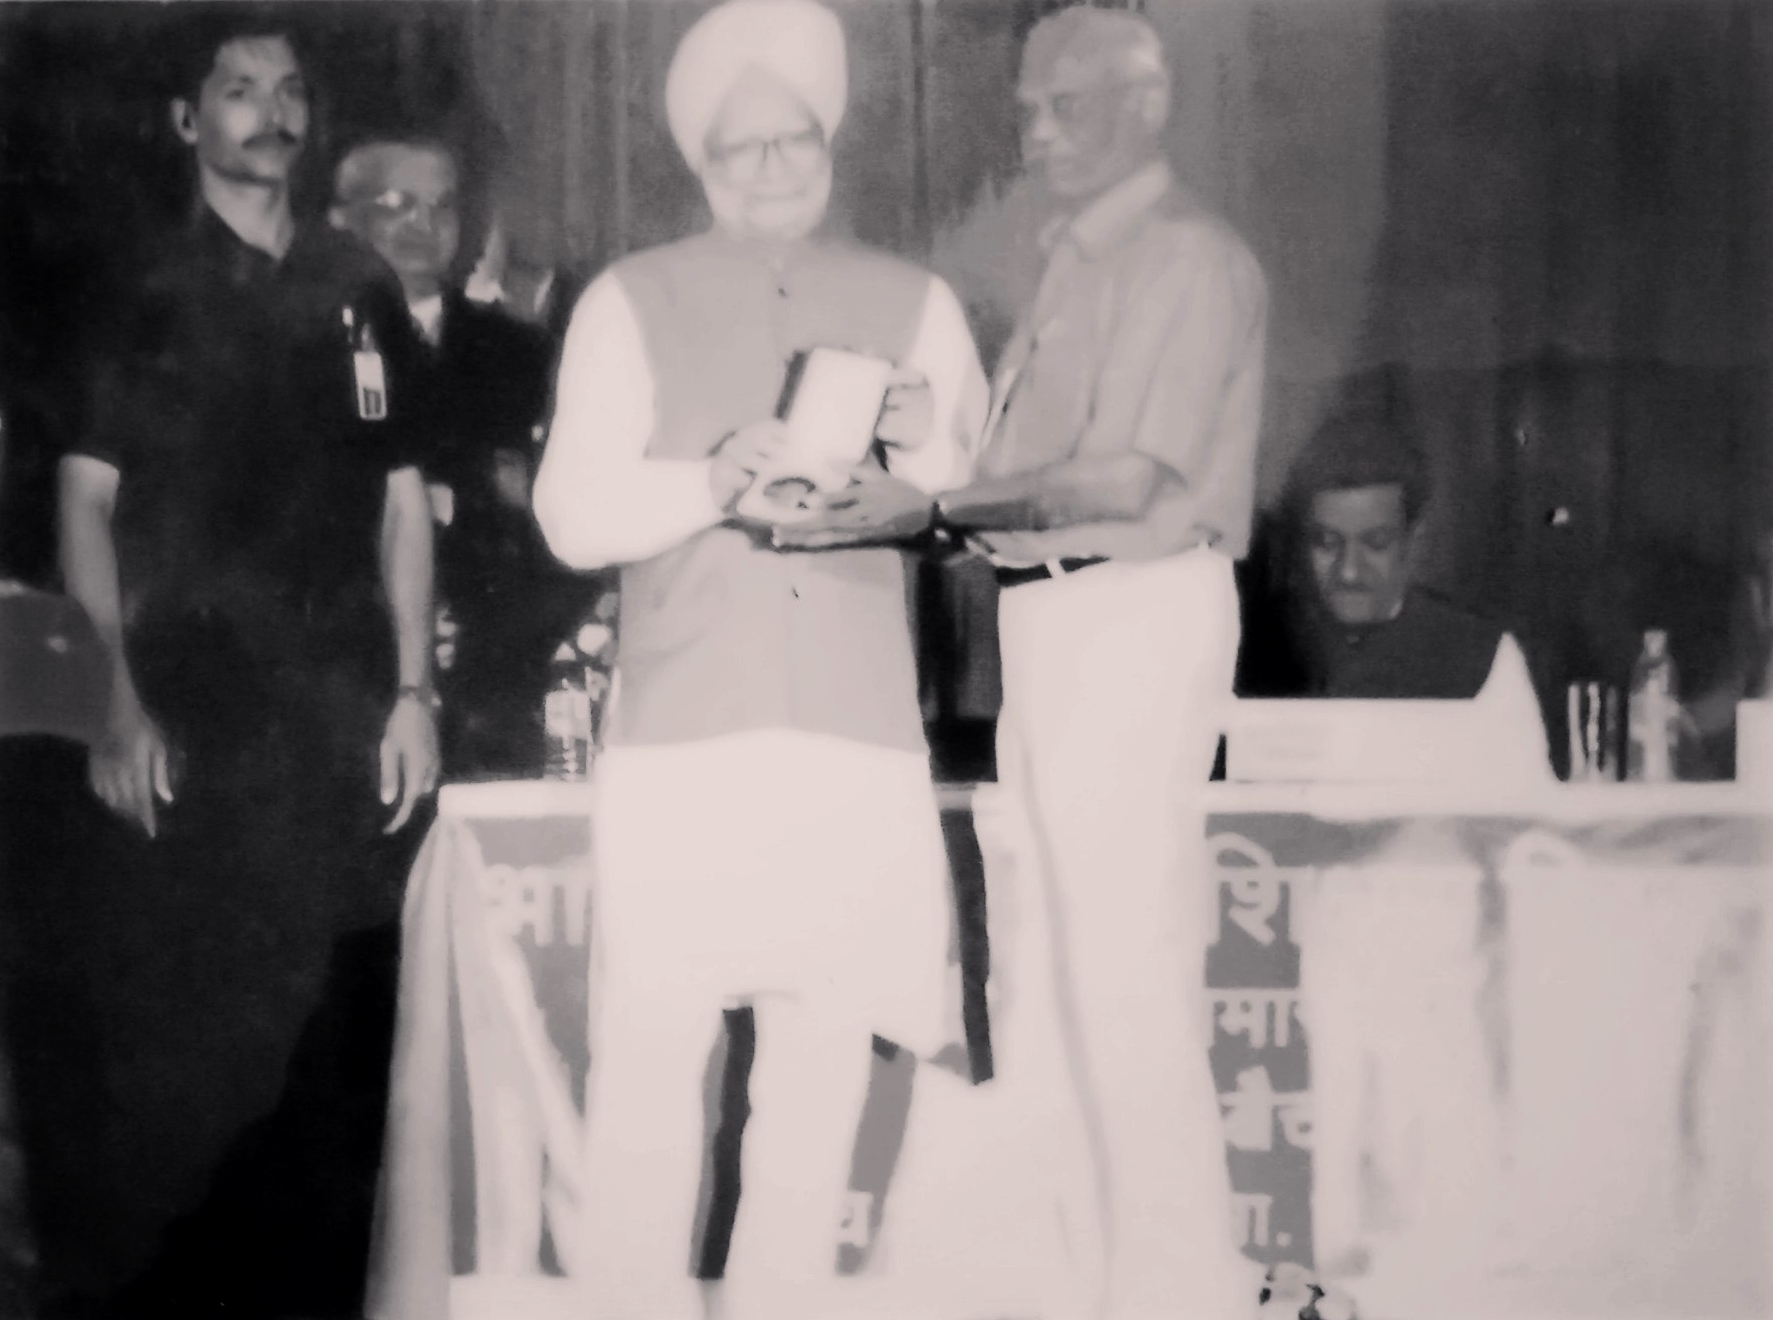
\includegraphics[width=0.7\textwidth]{Rajaji-04.jpg}
\caption{Prime Minister Manmohan Singh presenting the Homi Bhabha
gold medal, 2007.}
\end{figure*}

\chapter*{Routes to Enlightenment!}

Those of us who chose TIFR were taken to visit the experimental 
laboratories in TIFR. I found that all the laboratories were stacked 
with huge electronic boxes. Those days all electronic instruments used 
thermionic valves and hence were very big. I was thoroughly discouraged. 
I had a dread of electronics since my bad experience in MCC. So although 
I liked experimental physics, I had to do theoretical physics.

\section*{Tata Institute of Fundamental Research I (1958 to 1961)}

But for theoretical physics also I had a problem. Theory needs maths in 
which I was poor. So when I went to see KS Singhvi, the head of the 
theory group, I told him that I wanted to do theoretical physics, but I 
am not sure since I was not good in maths. He said he does not know any 
mathematics! So I joined Theory.

A few trainees who joined Theory group in the early years were Sudhanshu 
Jha and K V L Sarma both from the first batch and Mukunda and Divakaran 
from the second batch. The atmosphere for study was very good and there 
was hardly any restriction on what we can do. There were occasional 
lectures and seminars which we attended.

Since my mind was bent on understanding physics at its most fundamental 
level, I first took up the study of Quantum Mechanics, since my 
knowledge of it was not strong. For any question that I asked, the 
answer was in Quantum Mechanics. I sat with L I Schiff's book for many 
months and mastered it. The other books I liked were PAM Dirac, the 
Bible of QM, Pauling and Wilson, an easy-to-understand book and Heitler, 
a very beautiful tiny book.

Then I turned to Nuclear Physics since that was the most fundamental 
subject at that time. I read Bethe and Morrison and then Blatt and 
Weisskopf. Went to Kailash Kumar and George Abraham for guidance. The 
former put me in contact with many body theory and the latter in contact 
with few body problems. Abraham even suggested a specific problem. He 
asked me to redo the deuteron and triton structure using the recently 
discovered hard-core repulsion between nucleons.

I was not satisfied. I realized that the force between the nucleons 
comes from a deeper layer of reality which can be understood only from 
the then-new area called particle physics. There was no particle physics 
research in TIFR at that time. B M Udgaonkar (BMU) started studying 
hypernuclei which was in between nuclear and particle physics. 
Hypernuclei are nuclei in which one nucleon is replaced by a lambda 
particle. He introduced me to this subject and also to a few excellent 
reviews by Enrico Fermi on quantum theory of radiation and isospin 
symmetry.
 
He introduced me to Isospin and I calculated the ratio of Lambda going 
to $p + pi^-$ and $n + pi^0$ by using spurion technique. I thought it was a 
new result that I derived, but of course it was already well-known.
 
Udgaonkar was an excellent teacher. He had taught our batch of trainees 
reactor physics and the second batch quantum mechanics. Bhabha had sent 
him to France to learn about reactors, but BMU shifted to particle 
physics after returning.

Soon SN Biswas and LK Pandit joined and real particle physics started in 
the Theory Group. I started reading particle physics and learnt that the 
real theory of particle physics was Quantum Field Theory (QFT). So 
finally I reached the destination of my ``Inward Bound" journey.

I took up Bethe and Schweber's QFT and Jauch and Rohrlich's Theory of 
Photons and Electrons. I really loved the systematic treatment of QFT in 
Wentzel's book. I took it during my vacation in Kamuthi and read it even 
during the long train journeys.

My learning of QFT was systematized and consolidated only after I 
listened to LK Pandit's course of lectures on QFT. I was so impressed by 
his excellent lectures that I felt I achieved ``Enlightenment". I still 
remember lecturing to my friend Sudhanshu Jha on QFT during one of our 
evening walks along marine drive describing how I achieved my 
enlightenment. Maybe he was bored!
 
Soon I began to interact with Biswas and listened to his excellent 
lectures on integral equations. I was very impressed that an integral 
equation can be easily solved if the kernel is separable. Combining my 
knowledge of hypernuclei learnt from R H Dalitz's papers with a 
separable kernel as the potential between lambda and nucleon was very 
easy thing to do, with Biswas's guidance. Thus was born my first 
research paper and we proved Gell-Mann's Global Symmetry which simply 
equated all the eight meson-baryon coupling constants did not work.

Dallaporta visited TIFR and gave a series of lectures on the Symmetries 
of Hadrons. This was in 1960 before SU(3) came and he mainly talked 
about Gell-Mann's Global Symmetry. Gell-mann came to the correct SU(3) 
symmetry in 1961 only after many wrong attempts! Mukunda and myself took 
notes of Dallaporta's lectures that came out as a TIFR yellow report.

Heitler came and lectured on nonlocal QFT. Divakaran and myself took 
notes and brought it out as another TIFR report.

Gyan Mohan gave a beautiful series of lectures on QFT in Heisenberg 
picture and the LSZ form of the S matrix.

We were living in the servants' quarters attached to the Old Yacht Club 
where TIFR and AEET were situated, near Gate Way of India. This was the 
hostel of TIFR! One morning when I woke up, I was horrified to find that 
my finger-tips were of flesh colour. Mice had nibbled at them and 
removed flesh. They had done so with so much care that I was not 
awakened!

Bhabha had appointed an ex-ICS officer Mr EC Allardice, a Scotchman, 
as the Deputy Director (Administration) of TIFR. Seminar notices were 
put on the notice boards only after he approved them. Once a notice 
about a seminar on ``Odd-odd nuclei" was sent to him. Odd-odd, even-even, 
even-odd are technical terms in Nuclear Physics. Allardice said `` These 
Indians! tunda-tunda pani, garam-garam chai". So saying, he cut off one 
``odd" from ``Odd-odd" and sent it for the notice board!

I went on trekking in the western ghats with my friends who were senior 
to me: C S Warke, Biswarup Banerjee and K K Gupta. Once we were on a 
hill and I could see a long thing in a far-away hill moving. Obviously 
it was such a huge python which was visible from the next mountain!
 
On one such trip a funny thing happened. It was getting late and we 
wanted to take a short cut. One of us (KKG) suggested that we could cut 
the distance if we go through a railway tunnel. We were inside and it 
was dark. Suddenly we saw some light in the distance and we were happy 
that we were near the end of the tunnel. But the light grew bigger and 
bigger and we realized it was an approaching train! We were mortally 
afraid. It was a very narrow tunnel. There was space only for the 
railway track. All of us quickly hugged the tunnel wall. After the train 
passed, we thanked our stars and returned home, covered by soot and 
dust.

In those days, I used to see many films, sometimes more than one in a 
single day. English, Tamil, Hindi, even Marathi films! Those were really 
care-free days. There were two friends who were my constant companions. 
One was KG Nair a first batch trainee who intruduced me to the pleasures 
of PG Wodehouse. The other was VS Arunachalam who later rose very high 
in the DAE hierarchy.

There was an euphoria in the air. Remember only a decade had passed 
since Independence and there was an expectation of great things. I felt
      ``Nehru was in Delhi and Bhabha was in Bombay
       And all was well with our world". 
So my life and research would have gone on happily, but that was not to be.

One day Biswas told me that I must go to USA for PhD. I did not want to 
go; I did not think PhD was necessary for research. Those days PhD was 
a rarity. In MCC. Dr MA Thangaraj had great respect because of his 
doctorate degree, but most faculty members did not possess PhD degree. 
Also BMU in TIFR was not a PhD. But Biswas said that it was the policy 
of the Theory group to send young people for PhD. Biswas suggested that 
I should go to Maryland University. He liked Maryland University because 
JS Toll who had written some good papers on Dispersion Relations was 
there. He got the application form from Maryland. I was about to fill it 
when he came and said MGK Menon wanted to see me.

I went and saw him. He asked me why do I want to go to Maryland? I said 
I did not want to go, but Biswas asked me to go. He said I must go to 
Chicago University. He got the application form from Chicago and I 
filled it. Soon R H Dalitz was to visit TIFR and it was arranged that I 
must go to Chicago and work with Dalitz. TIFR packed me up and sent me! 
They bought the tickets, got the passport and visa.

Before that, I must describe what I call ``The Bangalore Event". In the 
summer of 1961, the Summer School of TIFR was held at the campus of 
Indian Institute of Science, Bangalore. Gell-Mann and Dalitz were the 
lecturers and the audience consisted of students like me and many 
stalwarts like Homi Bhabha, MGK Menon, SN Biswas, LK Pandit, Virendra 
Gupta, Yash Pal and Alladi Ramakrishnan.

Gell-Mann lectured on his Eightfold Way version of Sakata's SU(3) 
theory, fresh from the anvil, even before publication. In Gell-Mann's 
Eightfold Way, proton, neutron and lambda were no longer a triplet, but 
a part of an octet.
 
During one of the lectures Dalitz asked him why was he ignoring the 
triplet which was needed to define the SU(3) symmetry. Gell-Mann evaded 
a direct answer in spite of Dalitz's repeated questioning.

If Gell-Mann had answered Dalitz's question, quarks would have been born 
there in Bangalore, instead of having to wait for another three years. 
If any of us had answered the question, that would have been a major 
Indian discovery. This was a missed opportunity.
\begin{figure}[h]
\centering
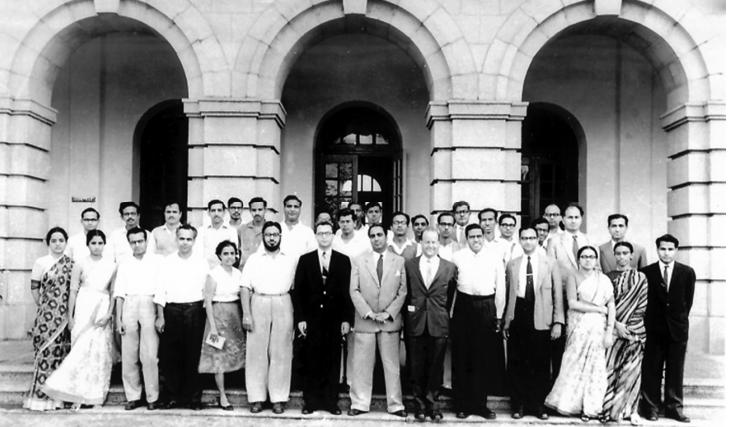
\includegraphics[width=\textwidth]{Rajaji-gellmann.jpg}
\caption{Bangalore Summer School 1961
L to R: First row: Thunga (Alladi's student), Indumathi (Alladi's
student),V Gupta, Yash Pal, Kharas (MGKM's secretary),MGK Menon,
Gell-Mann, Bhabha, Dalitz, Alladi, Jallihal (Administrator),
Radha (Alladi's student), Bhamathi, KK Gupta
Second row: AP Balachandran, G Ramachandran, PP Divakaran (behind
MGKM),GR (behind Bhabha), SN Biswas and LK Pandit (both between
Alladi and Jallihal)}.
\end{figure}
 
I sailed from Bombay to Liverpool in UK in August 1961 and flew from 
London to Chicago. The ship journey in SS Caledonia of Anchor Lines took 
about two weeks stopping at Karachi, Port Sudan and then at Alexandria 
in the Suez Canal. We were allowed to land at all the ports and go into 
the city. At Port Sudan a few of us went to see a Hindi movie. On the 
way we met a Sudanese and asked him about the way to the theater. He 
looked at us, asked whether we are Indians. We said yes and he replied 
that he will not help us! While the ship was passing through the Suez 
Canal we made an in-land journey to Cairo and had a sight-seeing tour of 
the pyramids and the famous Cairo Museum.

I had planned to write the Candidacy Examination once I reached Chicago. 
So I spent the time in the ship preparing for that. I could revise 
whatever I knew in physics using the excellent book by Kompaneets which 
presented all of Physics in a capsule form.

\section*{University of Chicago (1961 to 1963)}

On the first day at Chicago University I had a pleasant experience. I 
came out of the International House where I was staying and asked a 
gentleman about the direction to the place where the inaugural meeting 
for beginners was to be held. He said he was also going there. We walked 
together. Imagine my surprise that he went to the stage to preside over 
the meeting! He was Beadle, a Nobel-Prize winner in biology and the 
President of the University.
    
Soon I wrote the dreaded Candidacy Exam and passed. It was considered a 
tough exam and some of the questions were the ones set by Enrico Fermi. 
Generally students took one year to clear it. But I was not a beginner 
since I had spent four years in TIFR. I was admitted into the PhD 
programme and I was also Research Assistant to Prof Dalitz. Apart from 
Dalitz, there were many luminaries - Nambu, Oehme, Sakurai, Telegdi, 
Wentzel and Chandrasekhar. I attended the lectures by all of them.

I was staying at the International House and once I was returning after 
midnight after completing the experiment which everybody had to do in 
the course, I was accosted by a group of black boys who asked for money. 
Fortunately I had some money in my pocket. I threw it at them and ran 
for my life.

Another time a group of us went to a Cinema Theater beyond the Midway 
and we were surrounded by hoodlums again. We ran into a Department 
store.

Such events were common those days in the area where the University was 
situated. I hear things are much better nowadays.

Since I was a vegetarian, I suffered. Those days it was very difficult 
to get veg food in USA. At the International house the only veg food was 
half-boiled rice and half-boiled cabbage. Eating that day after day, I 
got sick of it. What saved me was the pizza. Once I discovered that, 
everyday evening I phoned Nicky's Pizzeria and ordered for pizza. From 
that time, pizza has remained my favourite food!
 
One day, when I was coming out of the library in the physics department, 
I saw Chandrasekhar emerging from the office. I realized that I was 
lucky to be in Chicago University. When I learnt that he was giving 
courses in General Theory of Relativity (GRT) and later, on Mathematical 
Physics, I took both courses. At the beginning of the GRT course, he 
said that he was teaching GRT since he wanted to learn it. He was 
absolutely right. Until then he had not worked in GRT. A few years after 
that he had mastered the subject and wrote his masterpiece ``GRT and 
Black Holes". His Mathematical Physics Course was on generalized 
functions which he wanted to master and used it in studying Black Holes.

Although I had attended two courses of Chandrasekhar, I hardly 
interacted with him. Chicago University had many Indian students. He had 
not interacted with any of them, as far I knew. Basically, he was a shy 
person. So imagine my surprise when one day, we got a letter from him 
inviting three of us A P Balachandran who had completed his Ph D in 
Madras and came to Chicago as a post-doc of Dalitz, R Ramachandran, a Ph 
D student and myself. He sent detailed instructions on the train that we 
must take to go from Chicago to Yerkes, some 70 km away. He had 
positions at Chicago University and Yerkes Observatory.

He came to receive us at Yerkes railway station and took us to his home. 
His wife Lalitha cooked a tasty South Indian meal for us. He took us 
around to see the telescope. We then played some ball game in his garden 
while he took rest. After a while tea was ready and we watched the TV. 
On that day Edward Teller was giving evidence in front of a Government 
Committee about the H-bomb programme of the Soviet Union. He became 
emotional and we could see tears from his eyes. Chandra talked to us 
about Teller. Then the conversation shifted towards other topics like 
particle physics, the subject of three of us and the science situation 
in India in which Chandra was greatly interested. We returned to Chicago 
with the satisfaction of spending a whole day in the company of a great 
man.
  
I take pride in the fact that I taught AK Ramanujam who later became
a famous Kannada poet and translated Sangam Tamil poetry, some Tamil.
At that time he was working as a research associate in the Department
of South Asian Studies in the Chicago University. He felt that the
Tamil I spoke was closer to the old Tamil since I come from the
southern part of Tamil Nadu. He asked me to speak Tamil and recorded it.
He paid me by the hour!

Dalitz asked me to make some calculations on hyper-nuclear physics. 
Although most of the main work was done by him, he included my name as a 
coauthor in the two published papers. I told him that I would like to 
work on a core topic of Particle Physics. He agreed.

At that time the dominant school of thought was the S matrix philosophy 
of GF Chew. Proving Mandelstam's double dispersion relations was 
considered the biggest challenge. Reinhard Oehme lectured to us on the 
many-sheeted S matrix,

AP Balachandran who had already obtained his PhD in Madras and joined as 
Dalitz's post-doc was frightening students like me by talking about the 
theory of many complex variables and ``The Edge of the Wedge Theorem". He 
was very mathematically oriented.

Those days you either group or disperse. The former led to SU(3) group 
and the later led to Dispersion Relations. An interesting story about 
the proof of Dispersion Relations from Field Theory is the following:

\begin{itemize}

\item Feynman: What is Dispersion Relation? 
\item Wigner: What is Field Theory? 
\item Chew: What is Proof?

\end{itemize}
Dalitz showed me a preprint by Oakes and Yang who criticized the SU(3) 
work of Gell-Mann and Neeman on two counts:

\begin{enumerate}

\item The decimet baryons Delta (1238), Sigma (1320), Cascade (1520) and 
Omega minus (1672) occur as poles of the S matrix on different Riemann 
sheets and so, no smooth movement of them is possible to give a single 
pole in the exact SU(3) limit.

\item The mass-differences in the octet and decimet of particles are so 
large that no perturbative treatment is possible for the 
symmetry-breaking interaction to yield the Gell-Mann - Okubo mass 
formulae for their masses.
\end{enumerate}

I could immediately solve the first problem since I was already familiar 
with the different Riemann sheets of the S matrix, through the study of 
Oehme's papers. Solution was that there is a retinue of poles in 
different Riemann sheets corresponding to a single hadron. This was the 
discovery of what are now called ``Shadow Poles".

But instead of sending off our result to Physical Review Letters as any 
American physicist would do, the conservative Dalitz sent a letter to 
Oakes and Yang. And Dalitz followed by me went away to Oxford. Meanwhile 
a host of other authors published the discovery of shadow poles. Dalitz 
and myself wrote up the result and published it in Physics Letters B 
later.

The second problem of Oakes and Yang did not have such a simple 
solution. It required detailed calculations based on models and that 
formed the core of my Ph D thesis.

\section*{Oxford University (1963 to  1964)}

Dalitz decided to shift to Oxford University in 1963. Since my thesis 
work was almost complete, he gave me the choice of continuing at Chicago 
as his student or go to Oxford. I preferred the second choice and left 
Chicago.

I sailed from New York to London by the famous Queen Mary and completed 
the writing of my thesis in Oxford in 1964. Dalitz suggested that I must 
do post-doctoral work in some University in the USA, but I felt I must go 
back to TIFR since TIFR had sent me only for Ph D! So in the summer of 
1964 I sailed from Marseilles to Bombay by SS Vietnam, a French ship.

I must describe the three types of ships in which I have traveled. 
Since TIFR paid for my journey from Bombay, I traveled in a first class 
ship SS Caledonia. There were no classes and everybody was treated as a 
first class passenger. In fact the captain dined with us. There were many 
interesting games in which I participated and even won a prize (Nehru's 
``Discovery of India")! Although Queen Mary was a famous ship, Dalitz's 
research funds could pay only for a second class ticket, myself being a 
student. The third journey from Marseilles to Bombay was paid from my 
pocket and so it was a French ship SS Vietnam used to carry Vietnamese 
prisoners of war! But there were many students returning to India in 
that ship and so I had a pleasant time. On the way, the ship stopped at 
Barcelona in Spain and we could do one-day sight-seeing.

Much later, when I was in California visiting my daughter Uma and her 
husband, they took me to visit Queen Mary which was anchored at Newport 
near Los Angeles. It had been converted into a Hotel. We stayed there 
and saw all the parts of the ship which were forbidden to me as a second 
class passenger of that ship 50 years ago!

During my stay in Oxford I enjoyed the company of Rajat Bhaduri and PP 
Divakaran, both second batch AEET trainees. Rajat got his PhD in Canada 
and came to work as Rudolf Pierl's post-doc. Divakaran, after spending 
one year at Chicago as Dalitz's student, came to Oxford like me. There 
was also ES Rajagopal, a condensed matter physicist working at Clarendon 
Laboratory at Oxford. Both Rajat and Rajagopal were married and we had 
very good food in their homes. Panchrathnam (before his name became 
famous as Panchratnam phase) was also a frequent visitor to Rajagopals' 
home, but was generally very quiet during our conversations.

While at Oxford, Dalitz sent me to attend the Varena Summer School at 
Lake Como, Italy. I attended the lectures of TD Lee, CS Wu, Martinus 
Veltman and many others.

Also, while at Oxford. Rajat and his wife Manjushree invited me to join 
them in a trip through Europe. Asish Datta, a friend of the Bhaduris, 
was the driver of the car that we hired and I was the map-guide. We 
visited France, Switzerland, Germany and Italy. It was an enjoyable 
trip.
 
Actually when I decided to leave for Bombay, I had not yet obtained my 
Ph D degree! Dalitz sent my thesis to my Ph D Committee in Chicago. 
Meanwhile I detected an error in my thesis and decided to recheck my 
calculations using the big computer in TIFR. It turned out that 
everything done using the computer at Oxford was correct and only some 
approximate calculation that I had tried in order to check my Oxford 
calculation was wrong! So the thesis was perfectly correct. I left for 
Kamuthi only after I made sure of that.

The thesis committee consisting of Telegdi, Oehme and a few others sent 
me the questions by post and I answered them by post. So my viva (the 
so-called third oral) was conducted by post. I passed it and in due 
time, Chicago University gave me the degree.

\section*{Back to TIFR ((1964-1976)}

By 1964, TIFR had shifted to new buildings in Navy Nagar, Colaba from 
their temporary premises in Old Yacht Club near Gate Way of India. 
Bhabha planned the new building in such a grand scale that it is 
sometimes called the Tajmahal of Homi Jahangir Bhabha. We could work 
there in peace and comfort.

I married Suthandra Devi in 1965 soon after I 
returned from Oxford. Two daughters were born, Poongodhai in 1966 and 
Uma in 1972.
\begin{figure}
\centering
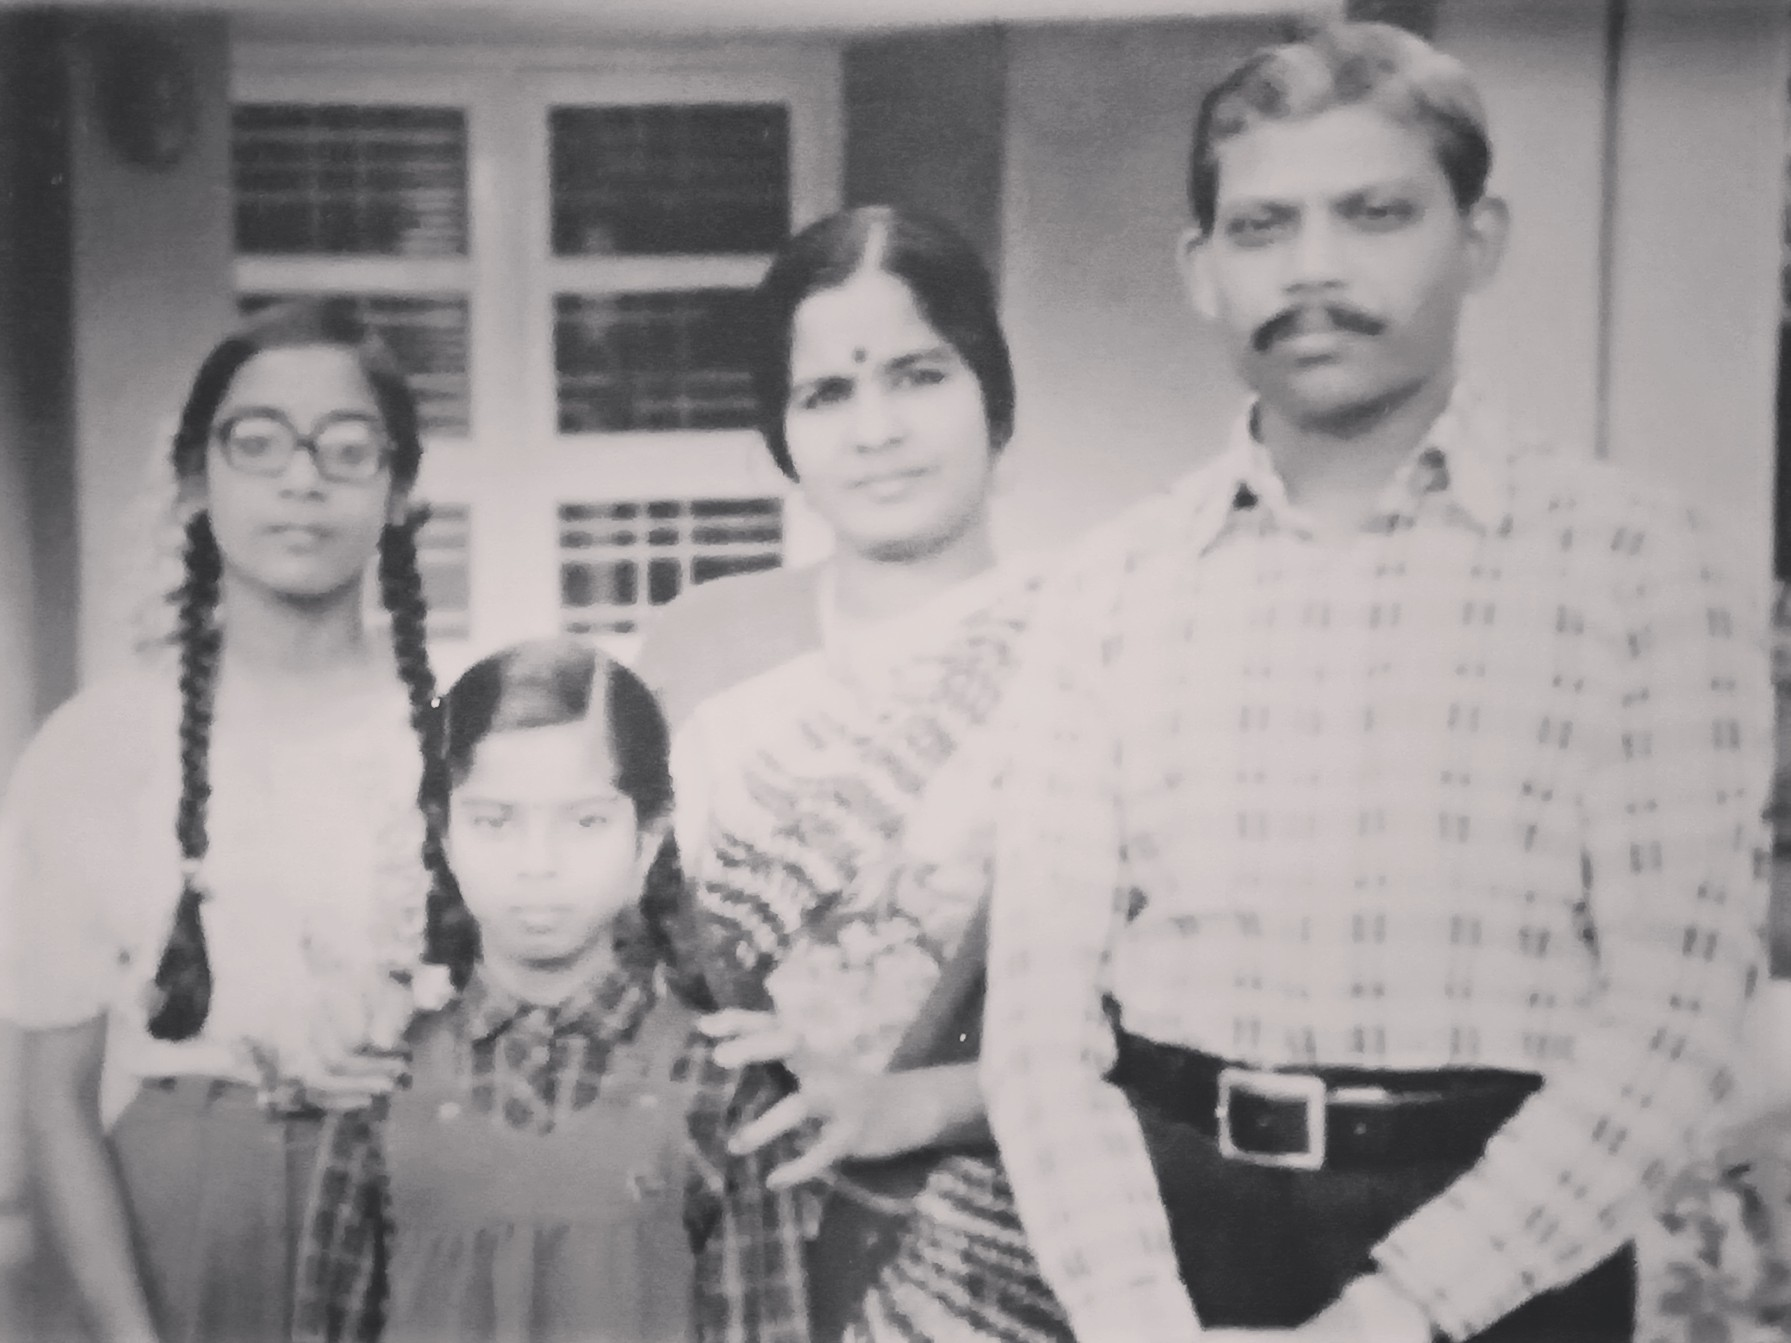
\includegraphics[width=0.8\textwidth]{Rajaji-03.jpg}
\caption{ Circa 1982, Poongodhai, Uma, Suthandra, GR.}
\end{figure}
Bhabha was killed when the plane in which he travelled crashed against 
Mt Blanc in Switzerland. So an era came to end. MGK Menon took over as 
Director of TIFR.

Soon after I returned to TIFR, I started teaching graduate students, 
although the formal Graduate School started only in 1969. Many bright 
students had joined. Among them were Sriram Sastri, Ashok Raina, Dipan 
Ghosh, Kailash Rustagi and Vinod Sahni (from BARC) and many others.

Willis Lamb visited TIFR and gave many lectures on the recently 
discovered Mossbauer Effect. Biswarup Banerjee and myself took notes and 
brought out a TIFR report.
                 
I went on a trip to the Himalayas with KKG, Biswarup and Luiz Balazs. 
Balazs was a theoretical physicist visiting TIFR. We went to Katmandu 
and from there we trekked. Our destination was the Valley of Flowers and 
Gosainkund Lake, which was sacred to Lord Vishnu. That was at 14,000 
feet. After reaching 13,000 feet or so, we reached the snow-line and we 
could not climb further since we were not equipped for snow. Further we 
were told there were no shelters for the night. On previous nights we 
stayed in the huts of the villagers and finally in a cave. Beyond this 
point not even a cave would be there. The sherpa who accompanied us 
refused to go further. So we decided to turn back. But one of us, 
Balazs, refused. He said we cannot turn back without reaching our 
destination. In fact he was suffering from diarria and could not eat 
anything. He was the most frail among us. Still he was adamant and 
wanted to climb further. While we admired his courage and tenacity we 
did not want our trip to end in a tragedy. We forced him to return with 
us.

This Balazs is a tenacious character. He was well-known for his 
bootstrap calculations which was part of the S Matrix Theory. This 
theory was reigning over particle physics at that time. Udgaonkar and 
Virendra Singh were very much in it.

To begin with, I continued my research along lines connected to my PhD 
thesis research. I showed that the hadron Lambda (1405) cannot be a 
three-quark bound state, but it is a composite of a baryon and meson, 
the so-called ``molecular hadron". I could construct a test for molecular 
hadrons. The test was simply that if it were a quark composite, the K 
matrix for meson-baryon scattering must have a pole but such a pole did 
not exist for K bar-N, pi-Sigma scattering. I talked about this result 
in two conferences, but did not publish in any journal.

I got into a controversy with my teacher Dalitz on the work on Lambda 
(1405), since earlier Dalitz, Wong and myself had worked on this hadron. 
Dalitz felt perhaps that he should be a coauthor in the K-pole paper. I 
wrote to him apologizing for what I did and explaining the circumstances 
in which this happened. Then I wrote a detailed paper making due 
references to Dalitz's work and also thanking him.

Much later after QCD came up, it was shown that QCD also supports the 
conclusion that Lambda (1405) is not a three-quark bound state.

Meanwhile Gell-Mann's current algebra was making progress and I worked 
on Current Algebra for a while with L K Pandit and Virendra Gupta.

In 1970, the HEP Conference was held in Kiev, Russia. I was one of the 
delegates chosen by TIFR. They got the visa and bought the ticket. They 
brought them to me along with a form to be signed by me. I was supposed 
to sign a bond to work in TIFR for a certain number of years because 
TIFR was financing my trip. I refused to sign. I told Udgaonkar who was 
the Chairman of the Theoretical Physics Section that under the 
circumstances I would not go for the Conference. They said it was a mere 
formality, but I said I was against signing any bond, on principle. They 
wanted to consult the Director, MGK Menon. He was out of town, but on 
return, instead of coming to TIFR, he stayed in the Tata House! So I did 
not go to Russia. Looking back, the whole thing appears to be silly 
since I did not have any intention of leaving TIFR and so the bond was 
only a formality. I have described this event only because this is the 
only time I fought with TIFR. Because of this fight, TIFR removed the 
requirement of the bond subsequently!

Maybe as a consequence of this fight, I undertook a pilgrimage. I 
visited the temples at Kanchipuram, Thiruvannamalai, Srirangam, 
Kumbakonam, Chidambaram, Madurai, Srivilliputhur, Thiruvananthapuram and 
Suseendram. This was the first time I visited them except Madurai. I was 
truly amazed at the cultural magnificence of Tamil Nadu.

\paragraph{Kolar events}:

One morning, my wife who was looking at the Times of India, exclaimed 
``Look, your friend KVL Sarma's name is in the front page!". I looked and 
found she had missed my name. The news item in the front page said G 
Rajasekaran and KVL Sarma have discovered a new particle. The Kolar 
experiments discovered some events that could not be explained. KVL 
Sarma and myself interpreted those events as due to a new particle. I 
also described this in an article in Physics News. TOI looked at only 
this popular science article and wrote the story. I was flabbergasted. 
There was no mention of the experimenters (that included MGK Menon). I 
contacted TOI and asked them to withdraw the story or at least correct 
it. They refused and said I can send a letter to the editor.

TOI could have verified the authenticity of their story by phoning TIFR. 
They didn't. This is the level of science reporting!

Recently at IMSc, MVN Murthy and myself have interpreted the 40-year old 
Kolar events as due to Dark Matter particles.

\section*{Gauge Theory}

I became aware of Yang-Mills (YM) theory by reading J J Sakurai's paper 
in Annals of Physics in 1959. That was the first paper in which YM was 
used in particle physics. Sakurai constructed a gauge theory of strong 
interactions. I continued to be interested in YM theory from that time. 
Veltman's lecture at Varena where he talked about the conserved weak 
current impressed me very much and I felt that weak interaction must be 
described by a YM theory. So, when Weinberg's paper on the SU(2)xU(1) 
electroweak theory came out in 1967 I had no doubt that was the correct 
theory. I read the papers of Goldstone, Higgs and Kibble.

In the subsequent two or three years, I lectured on these at various 
places including TIFR. In particular, in June 1971, I gave a series of 
lectures on the gauge theory of weak interactions including Yang-Mills 
theory, Faddeev-Popov ghosts, Higgs mechanism, electroweak theory, GIM 
mechanism etc. It came out as a SINP report. This was the first 
connected account of what became known as the Standard Model, anywhere 
in the world! It even contained my conjecture that the massless YM gauge 
quantum cannot exist as a particle because of the incurable infrared 
divergences (an early suggestion of what became known later as infrared 
slavery and colour confinement).

Nevertheless I failed to make any substantial contribution in gauge 
theory. This was partly because I had to take care of my sick father 
whom I had tried the treatments in the hospitals at Bombay and then in 
Madras, but to no avail. He passed away in May 1973.

I must refer to the peculiar circumstances under which I gave the gauge 
theory lectures at Saha Institute of Nuclear Physics (SINP) referred 
to above. In 1971, the whole of East Pakistan was in turmoil. Many 
refugees poured into Calcutta. Whole Calcutta was under siege. That is 
the time I went to SINP. Trilochan Pradhan who was my host made special 
arrangements for me. The driver who picked me up at the railway station 
was instructed to take a different route and take me to a different 
guest house. I was escorted with high security to SINP where my lectures 
were given. All over the City there were agitations and police shooting. 
Situation called for action by India. Indira Gandhi acted with a firm 
hand and Bangla Desh was born.
  
I became aware of t'Hooft's proof of the renormalizability of the 
electroweak theory which came out after my SINP lectures. Then came the 
discovery of asymptotic freedom of YM theory by Gross, Wilczek and 
Politzer and the construction of SU(3) colour gauge theory by Gell-mann, 
Fritzche and Leutwyler to describe strong interactions.

Renormalizability of electroweak theory and asymptotic freedom of YM 
theory are the two most important discoveries in Quantum Field Theory 
after the discovery of renormalizability of Quantum Electrodynamics in 
1947-49. I missed the boat in both, although I was well-placed with 
potential to contribute. I had already studied path integrals which 
t'Hooft used in his proof and was already giving lectures on Wilson's 
Renormalization Group and Callan-Symanzig equations which are the 
ingredients in the discovery of asymptotic freedom.

Although I missed the stage, I was sitting in the front row. I could 
catch their significance as soon as the discoveries came tumbling one 
after another! The years 1971-73 were truly exiting years. It was the 
watershed in the development of High Energy Physics.
  
Actually, until t'Hooft's proof, as far as I know, nobody except Joe 
Schechter in Syracuse University who added a U(1) to cancel the 
strangeness-changing neutral current and myself had taken Weinberg's 
theory seriously. Even after t'Hooft, only a few theorists took it 
seriously. Situation changed dramatically after the discovery of the 
weak neutral current interaction in the CERN experiment by Perkins and 
others in 1973.

In 1969, TIFR's theoretical physics summer school was at Nainital. Some 
memorable events took place there. Both Geoffrey Chew and Francis Low 
lectured. Chew lectured on S Matrix Theory. I asked him a question: 
Since S Matrix theory addressed only strong interactions, what happens 
to weak and electromagnetic interactions? Chew gazed at the distant 
Himalayan peaks visible through the window for a few minutes and simply 
continued his lecture.

Low lectured on the divergence problem of the Fermi theory of weak 
interaction and described all the methods proposed to deal with the 
problem. This was two years after Weinberg's paper. I asked Low at the 
end of his lectures why was he ignoring the Yang-Mills theory of weak 
interactions. He merely stared at me and refused to answer my question. 
He described seven or eight unnatural ways of solving the weak 
interaction problem but left out the one way that turned out to be the 
right way. To this day I have not understood how such a thing is 
possible, Low being a very experienced physicist. Somebody said it was 
because Low did not like Weinberg! Tapas Das and myself took notes of 
Low's lectures and brought it out as a TIFR yellow report.

\section*{Neutral Current}
Weak neutral current (NC) interaction is almost as strong as the usual 
charged current (CC) weak interaction but lay undiscovered all those 
years. It could have been discovered many years earlier if only the 
experimenters did not listen to some theorists who said NC cannot exist. 
The theorists thought that NC would lead to strangeness changing NC 
decays which were not seen, but they forgot that there could be 
strangeness non-changing NC. So the experimenters ignored some data which 
were actually due to NC. But the clinching experimental proof was 
possible only after the huge Gargamelle bubble chamber was constructed 
at CERN. Because of its size they could clearly distinguish a pion 
from muon and this was crucial for the discovery of NC through the 
absence of muon in neutrino collision.

As soon as the discovery of NC was announced, KVL Sarma and myself 
produced the first model-independent analysis of deep inelastic data. JJ 
Sakurai called our equations ``Master Equations". His analysis of elastic 
scattering coupled with LM Sehgal's of single pion production using the 
Master Equations led to the complete determination of NC coupling 
constants.

The evolution of the name starting from Gauge Theory is interesting. As 
soon as t'Hooft showed the renormalizability of electroweak theory I 
calculated the radiative correction to muon decay and sent it to 
Physical Review for publication. I had put the title as ``Radiative 
correction to the muon decay in gauge theory". Physical Review changed 
it to ``Weinberg's gauge theory". In 1972 the HEP Conference was held at 
Chicago that I attended. That is where gauge theory was presented as a 
Rapporteur's talk for the first time. BW Lee gave the talk. He called 
the theory as ``Salam-Weinberg gauge theory". Salam and Gell-Mann were 
sitting in the first row and I happened to be sitting in the second row 
just behind Salam and Gell-Mann. As soon as Lee mentioned 
``Salam-Weinberg gauge theory", Gell-Mann gave a nudge to Salam with his 
elbow. Later when the Nobel Prize was given, Glashow's name was added 
and the theory became Glashow-Salam-Weinberg theory. This is certainly 
justified since Glashow was the first to discover that SU(2)xU(1) was 
the correct gauge group for electroweak theory and also he was one of 
the inventors of the Glashow-Iliopoulos-Maiani (GIM) mechanism to remove 
the strangeness changing neutral current. However I now prefer to call 
it the Electroweak Theory!

\section*{Integrally charged quarks}

There is the possibility of quarks having integral charges unlike the 
Gell-Mann - Zweig (GZ) quarks which are fractionally charged. The former 
were introduced by Han and Nambu (HN). Probir Roy and myself constructed 
a colour gauge theory based on HN quarks and we got two interesting 
results. Although HN quarks have integral charges, as observed in deep 
inelastic scattering they will appear as fractionally charged. Further 
in this theory gluons are electrically charged and hence they also 
contribute to deep inelastic scattering. We published this in Pramana 
and soon we saw a preprint by Pati and Salam who also had the same 
theory. Although they also obtained the correct theory, they missed the 
fact that gluons in this theory are charged and hence contribute to 
deep-inelastic scattering. We pointed this out to them. Immediately 
Salam sent us a cable saying they were wrong and we were right. They 
also corrected their paper.

Subsequently, after I shifted to Madras, with my students and 
collaborators (T Jayaraman, Lakshmibala and Saurabh Rindani) I tested 
this theory by comparing the results with experimental data on deep 
inelastic scattering and electron-positron collisions. The theory agreed 
with data and could not be ruled out.

To this day this theory of HN quarks has not been ruled out by 
experiment and may even be the correct theory. Colour is broken in this 
theory spontaneously.

\section*{Visit to Hawaii}

In 1974 my friend Sandip Pakvasa invited me to visit him at Hawaii 
University. Since I had two young children, I hesitated to undertake the 
travel. It was my friend C S Warke who said it would be a good 
opportunity for the family to see USA. I travelled with my wife and 
children. Spent two very interesting months in Hawaii and worked with 
Sandip. In October 1974, the earth-shaking news came. That came to be 
known as the psi particle later. At that time we only knew that some 
extraordinarily narrow peak had been seen in electron- postitron 
collisions. It was as if anthropologists stumbled upon a group of humans 
in some remote corner of the world who lived for 100,000 years! After 
that there was no peace! San Fu Tuan was constantly at the phone trying 
to get more information on the narrow peak from Stanford and other 
Centres. He, Sandip and me wrote up some dozen interpretations for the 
narrow peak and published it. This is one of the earliest papers on the 
subject. Fortunately we did include the one correct interpretation 
namely the psi particle was a bound state of a charmed quark and the 
corresponding antiquark.

After Hawaii, I took my family on a tour of mainland USA visiting UCLA, 
University of Texas at Austin, Rochester University, City College of New 
York, Maryland University and Syracuse University. In all these places I 
gave seminars.

\section*{How we proved three Nobel Laureates wrong!}

1.By discovering the ``shadow poles" Dalitz and myself proved CN Yang 
wrong.

2.By working out the Han-Nambu model correctly, Probir Roy and myself 
pointed out the error of Abdus Salam and Jogesh Pati.

3.After I returned to TIFR in 1964, the discovery of CP violation by 
Cronin and Fitch excited the particle physics world. During his visit in 
Caltech, Virendra Gupta (VG) published a paper in Physical Review 
Letters in which he had constructed what looked like an elegant model 
for CP violation. After his return to TIFR he discussed this with me and 
I discovered that his model violated CPT theorem and hence is not 
tenable. This was the shortest paper I ever published. Since in his 
paper VG had thanked Gell-Mann for discussions, he is the third Nobel 
Laureate I proved wrong!

I have to balance the above by the following.

\section*{My failed attempts}

1.This was soon after I joined TIFR in 1958. In the primordial nucleon 
synthesis there was a gap. In the successive cooking of nuclei starting 
from proton by absorption of a neutron, there seemed to be a gap at A = 
5 because $He^5$ is not bound. When I learnt that the hyper-nucleus 
Lambda-$He^5$ is bound, I thought that is the solution. I discussed it 
with Udgaonkar, but it did not work.

2.After CP violation was discovered from K decays into two pions in 
1964, I thought the ugly CP violation can be avoided by recognizing that 
since pions are quark-antiquark bound states, Bose statistics for pions 
is only approximately valid and without Bose statistics, CP violation 
cannot concluded. This idea too did not work.

3.During 1964-64, with Arvind Kumar who joined me as a student, we 
undertook a massive calculation aiming to construct a complete theory of 
hypernuclei. In fact Arvind Kumar managed to do an enormous amount of 
calculation. It did not lead anywhere.

4.I tried to generate the nucleon-pion coupling using the quarks of 
which N and pi were made. This also did not lead anywhere.

5.For quite a long time,I imagined quarks to be leptons. That would have 
been the natural explanation for quarks and leptons satisfying the same 
current algebra. I tried to construct a mechanism by which the weakly 
interacting leptons could sometimes exhibit strong interactions, but I 
failed.

6. During 1967-70, I tried to construct strong interactions from weak 
interactions. by using the divergences of Fermi's weak interaction 
theory. TD Lee had shown how the quadratic divergences could be turned 
to strong interactions. Gell-Mann, Goldberger, Kroll and Ruderman wrote 
a nice paper showing how the quadratic divergences generate the diagonal 
(that is, the parity conserving strangeness conserving) sector that 
could be identified as the strong interactions. My aim was to redo these 
calculations using the YM theory of weak interactions of Weinberg's 1967 
paper. But alas! t'Hooft proved the renormalizability of Weinberg's 
theory.

\section*{University of Madras (1976 to 1984)}

Everything was going very well at Bombay. So why did I decide to leave 
Bombay? There are several reasons. For some time Shiva Sena was gaining 
ground. When there was water shortage, they even wanted to send back all 
Madarasis. One day there was a big agitation in the streets. When I was 
waiting at Gymkhana for the TIFR bus, some goons got hold of one of my 
TIFR colleagues and beat him up. So I decided that when a chance came I 
must leave Bombay. Second reason was that my children hardly knew Tamil 
and my wife spoke only Tamil. So I felt that my children must grow up in 
Tamil Nadu. A third reason was that I felt I must use my knowledge to 
teach at a University. Those were the days when Indira Gandhi introduced 
the slogan ``Science for the People". B M Udgaonkar was advising that 
TIFR people must go to the universities to teach. But none of these is a 
strong reason. So I must attribute my shifting to Madras to fate!

First I was selected as a Professor at the Guindy Engineering College by 
VC Kulandaiswamy who was the Director of Technical Education at that 
time. Although the College was to be upgraded as the core of the Anna 
University to be formed, I felt it was not the proper job for a 
physicist.

I got a second chance when Madras University advertised for a 
Professorship in the Dept of Theoretical Physics. I applied and got the 
job even without an interview. But there were many difficulties. For one 
thing although the offer matched my basic salary, my total remuneration 
at the University was considerably lower than that at TIFR since at TIFR 
I was getting a large Dearness Allowance (DA) which was not available at 
the University. Malcolm Adiseshaiah increased the salary considerably to 
match my salary plus DA at TIFR. I decided to accept the offer and 
joined Madras University in July 1976.

At TIFR I was living at the comfortable quarters provided by the 
Institute. At Madras I was literally thrown to the streets. I had to 
change the rented apartment three times until I finally managed to buy a 
old house.

A comparison between TIFR and Madras University would be apt at this 
point. I had figures to show that at TIFR, for every thousand rupees 
spent on salary for an academic person, ten times that much was spent on 
infrastructure, including library, money for attending conferences etc. 
In this I am not including the comfortable living quarters that TIFR 
provided. At the University, absolutely nothing beyond the bare salary.

Here I must mention my friend V Radhakrishnan who helped me on many 
occasions. But for him I would not have survived in Madras. He was a few 
years senior to me and I knew him and his wife Kaveri even at Bombay. He 
was a student of KK Gupta.

At Bombay, many were the evenings when he used to take me to Chembur, 
Sion or Matunga to listen to heavenly Carnatic Music by Chembai 
Vaidhyanatha Bhagavathar, Ariyakkudi, Semmangudi, MD Ramanathan or the 
celestial MS Subbulakshmi.

At the Dept of Theoretical Physics, there was PM Mathews who was the 
Head and G Bhamathi, M Seetharaman, MD Srinivas and SS Vasan were the 
faculty members. Malcolm Adiseshaiah introduced many rapid changes. He 
introduced MSc teaching at the Departments. Until then MSc was done only 
at the Colleges. The starting of MSc coincided with my joining. There 
were many good students. He introduced the semester system, monthly 
meetings of all professors with the VC and rotation of the headship of 
the departments. Since I was the seniormost after Mathews, I had to take 
up the headship.

There was V Srinivasan who joined as a visiting member. He was a 
remarkable person. He became a good friend of mine and we worked 
together on many papers. I took SD Rindani as a new faculty member and 
JK Bajaj and V Sriram as post-docs under my UGC project ``Gauge Theory". 
T Jayaraman first and then Lakshmi bala who were MSc students became my 
PhD students. So we had a very active group.

During my stay in the University, the Department of Theoretical Physics 
was the venue for two activities. Bajaj wrote many papers on Grand 
Unification but got frustrated that the scale of that theory was far 
away from presently accessible energies. So he left Physics. Along with 
MD Srinivas and MS Sriram he founded a movement called Patriotic 
People-oriented Science and Technology (PPST) whose main theme was that 
unless we pay attention to Science and Technology done in India from 
ancient times, science will not take root in this country. They brought 
out a journal named PPST. The journal does not exist any more. But the 
three of them founded the Centre for Policy Studies at Chennai and 
another institution in Delhi.

The Department= proved to be the venue where Sriram courted Lakshmibala 
and married her!
 
One morning an official car came to my residence to pick me up. It was 
because of a case against the University. I had conducted a meeting of a 
selection committee for a research assistant's post and made the 
selection. The former occupant of that post went to the court claiming 
he should have been selected. So the University sent me to meet the 
advocate of the University. That was P Chidambaram who later on became a 
Central Minister. Chidambaram asked me whether the person was selected 
by a regular selection committee on the basis of the academic 
qualifications of the candidate. I said ``Yes" and he asked me to sign 
that as a written statement. I did so. Chidambaram said ``Professor, I 
will now take care of it." That was that. The court decided in the 
University's favour.

Two bright students from IIT, Kanpur wrote to me saying they wanted to 
join me as research students. One was Avinash Dhar and the other was 
Ramadass. I think they were advised by my friends HS Mani and R 
Ramachandran, both at IITK. Avinash came. The University did not have 
any research fellowship money and no hostel facility. Avinash used his 
own money and managed to stay somewhere. He survived for a few weeks 
this way. Meanwhile he got admission into TIFR graduate school and I 
advised him to go. Because of this experience, when Ramadass wrote to 
me, I told him to go to TIFR. Both of them are now senior academicians 
at reputed institutions.

Malcolm decided to quit in 1979 and the University plunged back into its 
original state. All the measures that Malcolm introduced were undone one 
by one. MSc was stopped. I was getting frustrated.

\section*{Japan (1980 and 1981)}

Advised by my friend Sandip Pakvasa, Hirotaka Sugawara of KEK Japan 
invited me. I went and spent two years (1980 and 81) there. KEK is the 
National Laboratory for High Energy Physics of Japan. Apart from 
Sugawara there were many other bright theorists such as Yoshimura and 
Kobayashi. I interacted with the experimental groups too. Yasumi, an 
experimental nuclear physicist who wanted to measure the mass of the 
antineutrino in the internal bremsstrahlung electron capture of Holmium 
asked me to join him as a theorist. I calculated the rate of this 
process. This was my only experimental paper.

I must say something about the Japanese physicists and students whom I 
encountered. Their dedication and capacity for hard work were 
incredible. Even physicists in their sixties and seventies used to work 
in their rooms or laboratories very late into the night.

I had taken my family of wife and two daughters to Japan, but sent them 
back during my second year so that the school education of Poongodhai, my 
elder daughter was not affected too much. While in Japan both my 
daughters went to a Japanese school and picked up considerable Japanese.

I had many friends in Japan. Among them I must mention Roger 
Bissionnette who was an engineer in accelerator science. We used to 
travel together in Japan during my second year there.

In Japan I learnt three things: car-driving, Karate and Japanese 
language. Although I learnt to drive a car, I could not undergo the 
driving test since that required considerable knowledge of Japanese 
language. So I was driving only within the KEK campus! While learning 
Japanese, I found many remarkable similarities between it and Tamil. Of 
course all these three things that I learnt in Japan, quickly evaporated 
after return to India!

While I was at KEK, a memorial meeting for Tomonaga (who had passed away 
recently) was going to be held at Kyoto. All of us in the Theory group 
went to attend that. Schwinger was going to give the memorial speech. 
The announced title was ``The two shakers of Physics". I thought the two 
shakers were Relativity and Quantum Mechanics. Schwinger pointed out 
that his Germanic name ``Schwinger" meant ``shaker" and ``Shin" in the name 
of Shin Itiro Tomonaga also meant ``to shake". So those are the two 
shakers! He gave an excellent speech telling us how Schwinger and 
Tomonaga developed QED sitting on either side of the Pacific, unknown to 
each other. It was war time and there was no communication. The parallel 
went further. Schwinger described how both independently developed the 
theory of wave guides and microwave cavities needed in war. Although the 
triplet Tomonaga, Schwinger and Feynman were involved in developing QED, 
Schwinger hardly mentioned Feynman. The only mention of Feynman was that 
Feynman missed the correct numerical factor in one of the higher order 
calculations!
 
I returned to Madras University in 1982 and was not happy. I felt sad 
that a lot of progress was taking place in High Energy Physics and I was 
stuck in this hole.

In 1982 I visited ICTP, Trieste. It happened that the W and Z bosons 
were discovered at CERN at that time. My friend Sandip Pakvasa informed 
me about the W discovery and I had the good fortune to convey that 
information to Abdus Salam when I met him. He was very happy and thanked 
me. All the time he was munching groundnuts!

At the ICTP canteen a few of us including a Pakistani physicist were 
discussing things and I mentioned the following. I said that Salam is 
the only scientist who could be the Director of an Institution and at 
the same time made top-class discoveries. He discovered Superspace. I 
also said in a comparable situation Homi Bhabha had to abandon his 
research while managing TIFR and DAE. Immediately the Pakistani 
physicist said that is possible only if you can manage two wives!

\section*{Some interesting events}

In 1963 I left Chicago for New York to take the ship for England. I 
wanted to visit my friend SV Rangaswamy at Philadelphia. At the New York 
bus station I was supposed to take the bus for Philadelphia. From inside 
the station I could see the bus about to start. I dashed for it, but was 
stopped with a loud crash. I had crashed into a glass wall. Immediately 
security men took care of me. My face and body were covered with broken 
glasses. The doctors attended on me and carefully removed the glass 
pieces from my eyes. They also treated the minor cuts. I was very much 
worried that I may have to pay for damaging the glass walls. I was told 
that it was the opposite; I can claim for the shock and injuries that I 
suffered. The glass wall did not have any lettering or other warning 
sign and so the bus station was liable to pay. But I did not want to 
make any claim. The security guards were with me and put me in the 
correct bus.

During my trip to USA in 1974 with my family we visited many 
Universities as I already described. I had bought air tickets for the 
whole trip involving New York, Hawaii, Los Angeles, Austin, Maryland, 
Syracuse and Rochester. At the Syracuse airport, at the check-in counter 
I was told that my ticket was not valid. We went on arguing, but the 
official did not allow us to board. Meanwhile my luggage was already put 
in the aircraft. I lost patience and shouted at the officials. I threw a 
tantrum that frightened everybody. But it worked. Since the plane had 
already left for Rochester, they put us in a tiny fore-seater plane. We 
reached Rochester and saw that our luggage was already waiting there.

When I was in Bombay, I traveled with Virendra Singh to attend the 
Conference on Few Body Problems organized by AN Mitra of Delhi 
University. We reached the airport very early in the morning. After 
checking in, we sat in the departure lounge and began our conversations. 
Our discussion was perhaps very interesting. We lost the sense of time 
and did not notice that departure of our plane was announced. After a 
while we noticed that we were the only two passengers sitting there. We 
saw through the glass door that our plane was in the runway. We ran past 
the security guards and when we were near the plane, the pilot saw us 
and began to move the plane. We ran after the taxiing plane. The 
security guards took us inside the airport.

We complained that we missed the plane since the announcements were not 
audible ignoring the fact that they were audible to the other 
passengers! Finally they found two seats in the next plane, but we had 
to buy them. Fortunately V Singh had his cheque book. At Delhi, we 
missed only the morning session.

After returning to Bombay, we wrote to Indian Airlines asking for the 
refund of the fare that we had paid for the missed flight. There was no 
response. In spite of our repeated appeals, Indian Airlines refused to 
pay. We then had a bright idea. We had used the official letterhead of 
TIFR. This time we sent a copy of that letter to JRD Tata, the Chairman 
of the Governing Council of TIFR and also the boss of Indian Airlines. 
In a few days, we got our money!

I lived in the TIFR quarters at Chembur during 1967 to 1970 and commuted 
for four years. The quality of construction of the flat where we stayed 
was very bad. One day a big piece of the ceiling fell on the bed very 
near the place where my three-year old daughter Poongodai was sleeping. 
I met Bhandarkar the Administrative Officer at TIFR and demanded that I 
be allowed to occupy the Colaba quarters which were almost ready. He was 
making some excuses for the delay and I shouted at him right and left. 
This happened in the fourth floor of TIFR. He was a tall well-built man, 
but he simply ran for life, unable to bear my onslaught. I chased him 
until he disappeared into one of the rooms at the end.

It seems I was quite a terror those days!

As a consequence of this event, I was allowed to occupy the new flat in 
Colaba. I was the first occupant with many facilities not quite on. For 
instance the lift will close after we are in and take us to the basement 
where the door would not open. But that is another story.

Since both my daughters lived in the USA, every year we visited them. 
Once the immigration officer at Los Angeles airport saw that I had an 
invitation to visit the University of California at Riverside. He turned 
to me and said,``Since you are a Professor of Physics, I want to ask you 
a question. Is Einstein the greater scientist or Hawking?" I 
said, ``Without question, Einstein!" He did not agree and we went on 
arguing for a while. Meanwhile he stamped my passport and I came out. 
Only when my daughter saw the passport, we realized the mistake. In my 
enthusiasm of argument I was not attentive and the officer stamped B2 
visa. He was supposed to give B1, otherwise I cannot be paid by the 
University. My daughter Uma said it can be changed at the immigration 
office.

Early morning next day, Uma drove me for an hour from Redlands to the 
Los Angeles immigration office where the line was long even that early. 
There were many Mexican immigrants whose entry is through Los Angeles. 
When my turn came, I told the officer about my problem. He said once the 
immigration officer at the port of entry stamps it, not even the 
President of United States can change it. I will have to go out of the 
country and while reentering I can change it.

Uma wanted to take me to the border town Tijuvana near San Diago. I was 
supposed to walk down and cross the border into Mexico and reenter. I 
vetoed the idea.

As an anticlimax, the secretary in the Physics Department paid me the 
money without looking at what was stamped in the passport.
      
\chapter*{Taking the plunge- The IMSc}

I knew Alladi Ramakrishnan the director of the Institute of Mathematical 
Sciences (IMSc). I had many friends there and I used to stop over there 
on my way to Kamuthi and give seminars.


As I have already said Alladi was a good teacher. He was a Professor in 
the old physics department of Madras University. The department was 
headed by the famous GN Ramachandran. Through the help of C Subramaniam 
who contacted Nehru who contacted Bhabha, Alladi founded IMSc. It is not 
easy to found an Institute. Full credit for that goes to him.


But whatever he did after that was not creditable. Apart from inviting 
famous physicists who happened to pass through India, he did nothing. He 
did not recruit active young physicists. His autocratic way of running 
the Institute did not attract good people. The institute consisted 
mostly of his own students. Once DAE came to know his mode of 
functioning, they cut the funds which added to his woes. He did not 
conduct proper selection committee meetings. Once a selection committee 
was announced. A selection committee member was stranded at the airport. 
Alladi prevented the meeting from taking place, by not sending the 
vehicle to the airport.

Even the faculty who were hired, were hired for 6 months or 3 months. 
His mode of functioning became worse after his son completed his studies 
and became a mathematician. After that Alladi's one-point programme was 
centered around his son only. I was a member of a selection committee 
convened by Alladi. MS Narasimhan was the chairman and Alladi's son 
Krishnaswamy was one of the candidates. When it was the turn of the 
committee to examine Krishna's case, we expected Alladi who was a member 
of the committee to withdraw. But he did not. The Chairman had to ask 
him to withdraw!

In 1983 I heard that the Director of IMSc, Alladi, was getting 
superannuated and he had to quit. But I never considered going to IMSc 
since it was worse than the University. It would be like jumping from a 
sinking ship onto a sinking boat. I had good contact with Udgaonkar and 
I had a good conversation with him on IMSc when we were in the same 
flight one day in 1983. A selection committee was set up to select the 
next director. Although I did not apply, the committee invited me for an 
interview. The Committee was chaired by V C Kulandaiswamy who had become 
the VC of the new Anna University. The other members were Udgaonkar and 
M S Narasimhan, the famous mathematician from TIFR. I went for the 
interview and I spoke frankly about the miserable state of IMSc and said 
if fresh blood could be infused, the Institute will survive.

I learnt that they had selected me. It was not clear to me whether I 
should be happy since I did not want to be an administrator although I 
did some administration as Head of the Dept in the University. I wanted 
to continue in physics.

Later I heard that ECG Sudarshan wanted to become Director and his 
friend Ramanna who was the Chairman of Atomic Energy Commission (AEC) 
decided to give the position to him. But apparently Sudarshan wanted 
also to hold his position in the University of Texas, Austin. So Ramanna 
wanted me to hold the fort at IMSc as a Deputy Director.

One day in 1983 I was informed that I must meet Ramanna. He was getting 
down from a military plane since he was the Defense Minister. I met him 
in the airfield itself. Ramanna said he had come only to meet me. Soon 
he was joined by Y S Das, the Additional Secretary. Both discussed the 
issue with me and tried to persuade me to accept the job. I was 
reluctant. The institute needed development and only a full-time 
Director can do it. How can I do it when the Director was sitting on the 
other side of the globe?

Later it seems that it was YS Das who solved the problem. Deputy 
Director cannot assume full powers. So they created the post of Joint 
Director and added this sentence in the constitution of IMSc: ``During 
the Director's absence the Joint Director shall have full powers of the 
Director".

Even then I was not very happy. Many of my friends (Virendra Gupta of 
TIFR, Kameshwar Wali of Syracuse University) who knew Sudarshan better 
advised me against the move. I was happy that Sudarshan's presence in 
Madras would brighten the academic atmosphere. I would have preferred 
his full-time presence as the Director of IMSc and I could continue in 
Madras University. Since I knew him as a friend, myself and others in 
the Department could derive considerable academic benefits. But that was 
not to be.

I knew Sudarshan well. My relationship with him was very good based on 
the high regard I had for him because of his top-class scientific 
achievement.In 1974 He invited me and my family to Austin, Texas. We 
spent two weeks there and he treated us like a royal family. Later 
during one of his Bombay visits, my high opinion came down a little 
because of the derogatory words he uttered about Mahatma Gandhi. My 
regard for him blinded me even to the wrong things about him that were 
said by others.

I got the appointment letter from the Tamil Nadu Government in October 
1983. But could not take a decision one way or the other. Meanwhile 
there was considerable pressure from DAE. Finally in February 1984, I 
took the plunge. There were five months between my receipt of the 
appointment letter and my acceptance of the job.

I went to the Institute and took charge from TD Sundararaj who was the 
Education Secretary of Tamil Nadu Government and who was officiating as 
the Director of IMSc. Alladi tried to extend his tenure by six months or 
at least by one month. But the Government did not give him even one day 
extra and made sure that Alladi really quits by asking Sundararaj to sit 
in the Director's chair!
 
%\section{Institute of Mathematical Sciences (1984-now)}

\section*{Building up IMSc (1984 to 1988)}

Once I decided to take up the job, I plunged into it with full force and 
commitment. When I joined, there were only 12 faculty members and 6 
students! Even after 20 years of existence the institute remained in the 
backwaters. Obviously recruitment was essential but that required many 
things to be done. Many developments had to take place. The following 
were taken up:
\begin{itemize}
\item Land for Hostel and Guest House,
\item Central Government salary structure and other benefits,
\item Recruitment of Faculty,
\item Graduate School,
\item MSc Programme (with Anna University),
\item Theoretical Computer Science.
\end{itemize}

I will now describe how these were achieved. 

When I see how hard it has become to get additional land for IMSc, I 
realize how lucky we were in 1984. Since my first priority was to 
recruit faculty at an all-India level and an vibrant Graduate School and 
an active visitors' programme, it was clear that the zeroth order step 
was to get land for the Hostel and Guest House.

Once I eyed the piece of land opposite to IMSc, where buffaloes were 
grazing, I determined to go ahead and get it. The fact that I had good 
relationship with both C Aranganayakam who was the Education Minister of 
Tamil Nadu and the Chairman of our Governing Council and VC 
Kulandaiswamy who was the Director of Technical Education and a top 
Educationist, helped in the quick transfer of the land to us.

The salary-cum-allowance structure as well as other service benefits at 
IMSc were hardly such as to attract brilliant scientists to join here. I 
was keenly aware of the wide disparities that existed between IMSc and 
other national institutes where the salary structure was that of the 
Central Government.

In spite of many discussions and Committees that were set up, nothing 
tangible came out. At the end of my first year at IMSc, I was quite 
upset that we could not implement this measure which was a precondition 
for the success of our recruitment programme.

I decided to force the issue and worked out a strategy. I met Ramanna. 
He was sympathetic and appreciated the need for prompt action. He agreed 
to sign the letter (drafted by me) addressed to Aranganayakam. I carried 
the letter personally to the Minister and explained the situation to 
him. His approval was very prompt and I knew that day that the battle 
was won. I announced the improved service benefits to the Faculty 
immediately. This was the way the Gordian knot of Committees and 
Subcommittees was cut.

There were still some hitches. For instance the administrative and 
service staff was still not covered by the new scheme. I took our 
Registrar G Sethuraman with me to meet Ramanna at Kalpakkam to convince 
him of the advisability of enlarging the scheme to the administrative 
and service staff.

As a result of these endeavours, all the obstacles were removed and our 
recruitments started in full swing. Of course the benefits were 
applicable to everybody, whether new recruits or existing members. Every 
member of IMSc got a substantial increase in his or her pay with 
retrospective effect. Many other welfare measures available in other 
central government institutions such as Leave Travel Concession, Medical 
Scheme could be implemented in IMSc soon after, since all these were 
regarded as part of the same package.

Further, once the status of the IMSc members to be on par with others 
governed by the central government system was granted, then the 
subsequent improvements recommended by the Pay Revision Commissions 
became automatically applicable to our members. These benefits are 
enjoyed by all of us now, thanks to the government of Tamil Nadu and 
DAE.

During these four years (1984 to 1988), the faculty strength grew from 
12 to 31. Both in Theoretical Physics and Mathematics we were able to 
attract very brilliant young people who became the pillars of IMSc in 
the subsequent years.

The close contacts that I had with various Centres in the country where 
good Theoretical Physics groups existed and similar contacts and even 
more importantly the stature that Seshadri enjoyed among mathematicians 
facilitated the recruitment programme. In fact most of the new faculty 
members in Theoretical Physics were known to me academically and all the 
new faculty members in Maths were known to Seshadri academically.

Along with the new faculty expansion, we recruited a large number of 
research students also. The total number of post-doctoral research 
fellows and research students increased from 6 to 35 in two years.

An important feature of the new recruitments must be stated and stressed 
here. In contrast to the original composition of IMSc before 1984 which 
consisted predominantly of members from a single state only, the newly 
recruited faculty and students hailed from various states spread all 
over the country. Thus IMSc achieved a truly national character.

Systematic post-MSc level courses for the research students working 
towards their Ph D degrees were started during this period, in all 
subjects coming under Theoretical Physics and Maths, since a sizeable 
number of students had joined as already mentioned.

Jagannathan and myself prepared detailed syllabi in all the subjects 
under Theoretical Physics. Jagannathan's keen interest in teaching and 
especially the meticulous care to detail that characterized all his work 
played a major role in putting the teaching of theoretical physics on a 
sound track. We thus laid the foundation for the Graduate School at IMSc 
that has flourished over the years.

From early on, it was clear to me that there was a serious gap in our 
graduate school. Although the School was primarily intended for post-MSc 
students, we had allowed ``exceptionally bright" post-BSc candidates also 
to apply. In fact there were a few who had only BSc, but were better than 
the best post-MSc students. It seemed a pity to send them back to 
college for another two years for getting an MSc degree.

I discussed this problem with VC Kulandaiswamy who had become the VC of 
the newly created Anna University. He had also appointed me as member of 
the Syndicate, Academic Council and the Board of Studies of the 
University.

He understood the issue and agreed to introduce a new degree called MSc 
(by research) in the University that can be run by IMSc faculty in 
collaboration with Anna University. Since I had been inducted into all 
University bodies it was possible for me to discuss with members of all 
of them and get the new degree approved.

This is how MSc started at IMSc and it functioned as a door to introduce 
``exceptionally bright" candidates into research, just after their BSc 
degree.

Starting of Theoretical Computer Science Research is another milestone 
in the growth of the Institute during 1984-88. In the pre-1984 period 
there was no Theoretical Computer Science group in IMSc. Such a group 
was formed after PS Thiagarajan joined IMSc in 1986. Soon other younger 
members joined and a strong TCS group has been flourishing at the 
institute.

Although I had full powers I knew about Sudarshan's ego. So I made it a 
point to discuss with him when he came after his stay in Texas, all the 
important steps taken by me and got them signed by him. In the beginning 
things went on smoothly. In fact many times he told me ``Rajasekaran, we 
seem to be thinking along the same lines!"
 
But as the years went by, things changed.

\section*{Turmoil(1989)}

Sudarshan spent less and less time at IMSc during the four years 84-88. 
Every year he spent half the year in Austin, Texas. Some years it was 
more. This would not have mattered much if the Joint Director had been 
allowed to function with full power. But Sudarshan's ego prevented that. 
Slowly he began to dislike everything I had done in his absence. He 
would come after a long break and make decisions inconsistent with what 
was done in his absence.

More importantly, selection of faculty was being held up. It was very 
difficult to have Selection Committee meetings during the period of his 
brief presence since other members who were busy could not come on those 
days.

Especially in Mathematics this became a serious issue. Seshadri insisted 
that I must act since I had the authority. So I conducted a Selection 
Committee meeting in Sudarshan's absence. M R Srinivasan was in the 
chair. I sent out the appointment letters. When Sudarshan learnt about 
this he was furious. I told him it was a duly appointed selection 
committee and I had authority to hold its meeting.

One of the candidates selected was V S Sundar, a mathematician. He 
joined. Sudarshan called him to his office and told him point-blank that 
he must quit since his appointment is cancelled. This must be an 
unprecedented behavior by the Director of any institution. Sundar left 
and rejoined only after Sudarshan was removed. He has done high-quality 
mathematics ever since.

IMSc had one faculty member representing the faculty in the Governing 
Council. So far KR Unni, was doing that and his term ended. Whom to 
appoint now? Earlier I think Alladi simply did it by fiat. I thought of 
doing it more rationally. There were two candidates, ND Haridass and 
Seshadri. Although I preferred Seshadri I decided there shall be an 
election. Seshadri was chosen unanimously. That also angered Sudarshan.

I must say something more about Seshadri here. From the beginning it was 
clear that Seshadri, being an eminent mathematician and involved in the 
actual recruitment of mathematical faculty in IMSc, must be made 
in-charge of the Maths group. This simple thing was resisted by 
Sudarshan. He wanted to play politics between Unni and Seshadri by not 
announcing that Seshadri was in-charge of the maths group.

Meanwhile Seshadri became FRS. It became a glaring injustice not to make 
him in-charge of the Maths group.

As for my relations with Alladi, in the beginning they were cordial. 
In fact after hearing that I was to take over, he threw a party to 
welcome me! The relationship got soured only because of his son. 
Krishna, while being on the rolls of IMSc as a faculty member, was 
almost permanently abroad. Once when his application for extending his 
leave came to me as the director-in-charge, I refused. Alladi himself 
phoned me repeatedly asking me to grant his son's application. I had to 
cut him short. From that time Alladi treated me as his enemy.
 
All these things accumulated increasing the tension in the Institute. 
But the event that toppled the apple cart is the dismissal of 
Sethuraman, our registrar. In the beginning years at IMSc I had 
struggled with the administration and I felt that a competent registrar 
is necessary. I went to Ramanna for help. He sent G Sethuraman from DAE 
as our registrar. I knew him since earlier he was the typist cum 
secretary in the Theoretical Section of TIFR. In fact many of my papers 
intended for publication were typed by him. He turned out to be an 
excellent registrar having good liaison with DAE.

Above all Sethuraman had unquestionable integrity. So he did not like 
some of the money dealings of Sudarshan which were shady and apparently 
will involve the institute also. Sethuraman expressed his misgivings to 
Sudarshan. The latter dismissed the former unceremoniously without giving 
any reason.

That was too much. I had to act. I sent a detailed report to M R 
Srinivasan who was the Chairman of the Governing Council (GOC) with 
copies to all the members. In the main I mentioned the continued absence 
of Sudarshan for months together and his erratic actions when he comes. 
I said I cannot hold the fort under these circumstances. Actually this 
is the first time that the GOC became aware of Sudarshan's absence from 
IMSc for long periods.

Sudarshan's reaction was violent and became more erratic. He cut off my 
official phone connection. He gave a kick to the door of my office room 
and removed my name plate.

I felt even my life to be in danger and wanted to be away from Madras. 
Both IIT Kanpur and IIT Bombay offered me refuge. The former sent me the 
appointment letter. Finally I decided to go to TIFR, vowing to return 
only after Sudarshan was removed. TIFR was a familiar place for me. Also 
I could watch what DAE was going to do.

In this struggle, most of the faculty supported me. In particular, there 
were Haridass, Baskaran, Thiagarajan and Balasubramaniam who were with 
me. Of course Seshadri was with me. Only the faculty who joined before 
1984 did not support because of their alleged loyalty to authority.

Thanks to TIFR I enjoyed peace for one year (1989). There I could return 
to Physics and complete some of the research projects.

Finally Sudarshan left at the end of 1989. He had to leave since his 
5-year term ended. But he went to the court against the institute 
claiming he was a permanent director. He quoted some statement of Indira 
Gandhi the Prime Minister as evidence. But he had signed a 5-year 
contract. He tried to hide that, but Sethuraman managed to unearth it 
and the judge threw that at his face and dismissed the case. Of course 
all this took time.

My sufferings were not over. He filed a criminal case against me citing 
the official letter I had written to the GOC as defamation. I had to 
fight it out. My lawyer told me that according to Indian law, if you 
call me a fool it is not defamation if you can prove it. So the 
lawyer asked the court to ask Sudarshan to produce his passport which 
will prove his absence. His lawyer went on asking for postponement for 
many months. My lawyer had advised me to be present whenever my case 
came up. His lawyer did not appear at all. So finally the judge 
dismissed the case.

All this took time, also money. Sudarshan could throw away a few dollars 
at his lawyer, but in my case it was my hard-earned money. Later IMSc 
offered to reimburse this expense, but I was not keen. Sudarshan's aim 
was only to torture me and he succeeded.

Let me mention two unexpected fall-outs from the turmoil.

Prof Seshadri left IMSc with a group of Maths and TCS people and founded 
what became known as CMI (Chennai Mathematical Institute). Thus a good 
thing can emerge from a bad happening!

A very strong group of high-energy-physicists, Anjan Joshipura, Saurabh 
Rindani and Utpal Sarkar, whom I had hired left IMSc during the turmoil 
and founded the HEP group at the Physical Research Laboratory 
(PRL),Ahmadabad. What was a loss for IMSc became a gain for PRL!

\section*{Back to peace and progress (1990-now)}

The Institute was put back on the path of progress in 1990. R 
Ramachandran took over as Director in 1990 and IMSc had a smooth sail 
after that. Thanks to him I could get back to academic activity. During 
his term and after Balasubramaniyam took over in 2000, the institute 
continued to grow and has reached great heights. Progress continues with 
the present Director V Arvind.

The following event might have happened in 2011 when the Golden Jubilee 
of IMSc was celebrated. The famous physicist David Gross who is a Nobel 
Laureate visited the Institute and went to Kolkata. I was also going to 
Kolkata and so we traveled together. His wife was with him. At the 
Chennai airport he wanted to wait at the VIP's lounge and wanted me also 
to be with him. In the lounge, there was Amartya Sen, another Nobel 
Laureate with his wife. Gross and Sen knew each other. So, for a while I 
was enjoying the company of two Nobel laureates!

But the story does not end there. After the plane took off, Gross came 
to me running and said ``Rajaji, I lost my laptop in the airport." At the 
security check-up he forgot to pick it up. Although the laptop was an 
expensive one, he was particularly worried since he had many valuable 
documents in that laptop. After we landed, from the Kolkata airport 
people it was difficult to get any help. Fortunately my friend R Simon 
from IMSc happened to have arrived at Kolkata airport at the same time. 
With his authoritative voice and gestures, he forced the airport people 
to make the connection to the Chennai airport. We got the news that the 
laptop is safe and will be sent to Gross in USA. Gross did receive it in 
due time.
\begin{figure}[h]
\centering
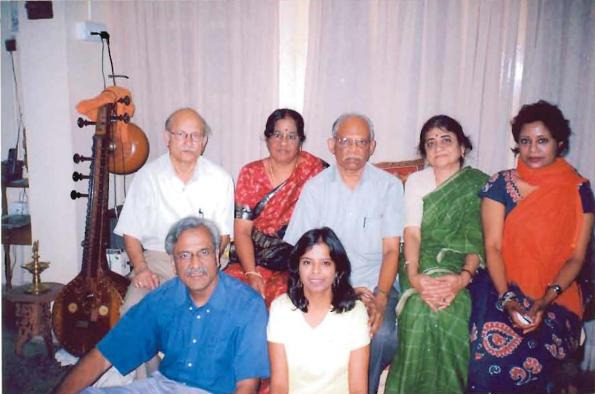
\includegraphics[width=0.55\textwidth]{Rajaji-family.jpg}
\caption{ L to R: Rajat Bhaduri, Suthandra, GR, Manju Bhaduri, Poongodhai.
Below: MVN Murthy, Uma.}
\end{figure}
\begin{figure}[h]
\centering
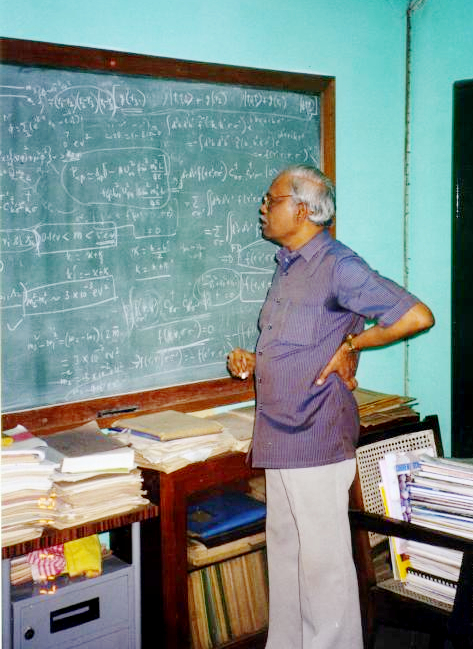
\includegraphics[width=\textwidth]{rajaji1.jpg}
\caption{At the blackboard in my old office.}
\end{figure}


\chapter*{Other Activities and Research}

\section*{Chennai Mathematical Institute (CMI)}

Seshadri founded CMI with Mathematics and Theoretical Computer Science. 
Even before IISERs came, Seshadri admitted into CMI talented students 
after school so that they can pursue their studies in an atmosphere of 
research. He wanted CMI to grow into a full-fledged University and as a 
first step wanted to have Physics. He asked me to help in Physics 
Faculty recruitment and teaching. I have been doing that. We now have a 
Theoretical Physics Group of outstanding young faculty members.
\begin{figure}[h]
\centering
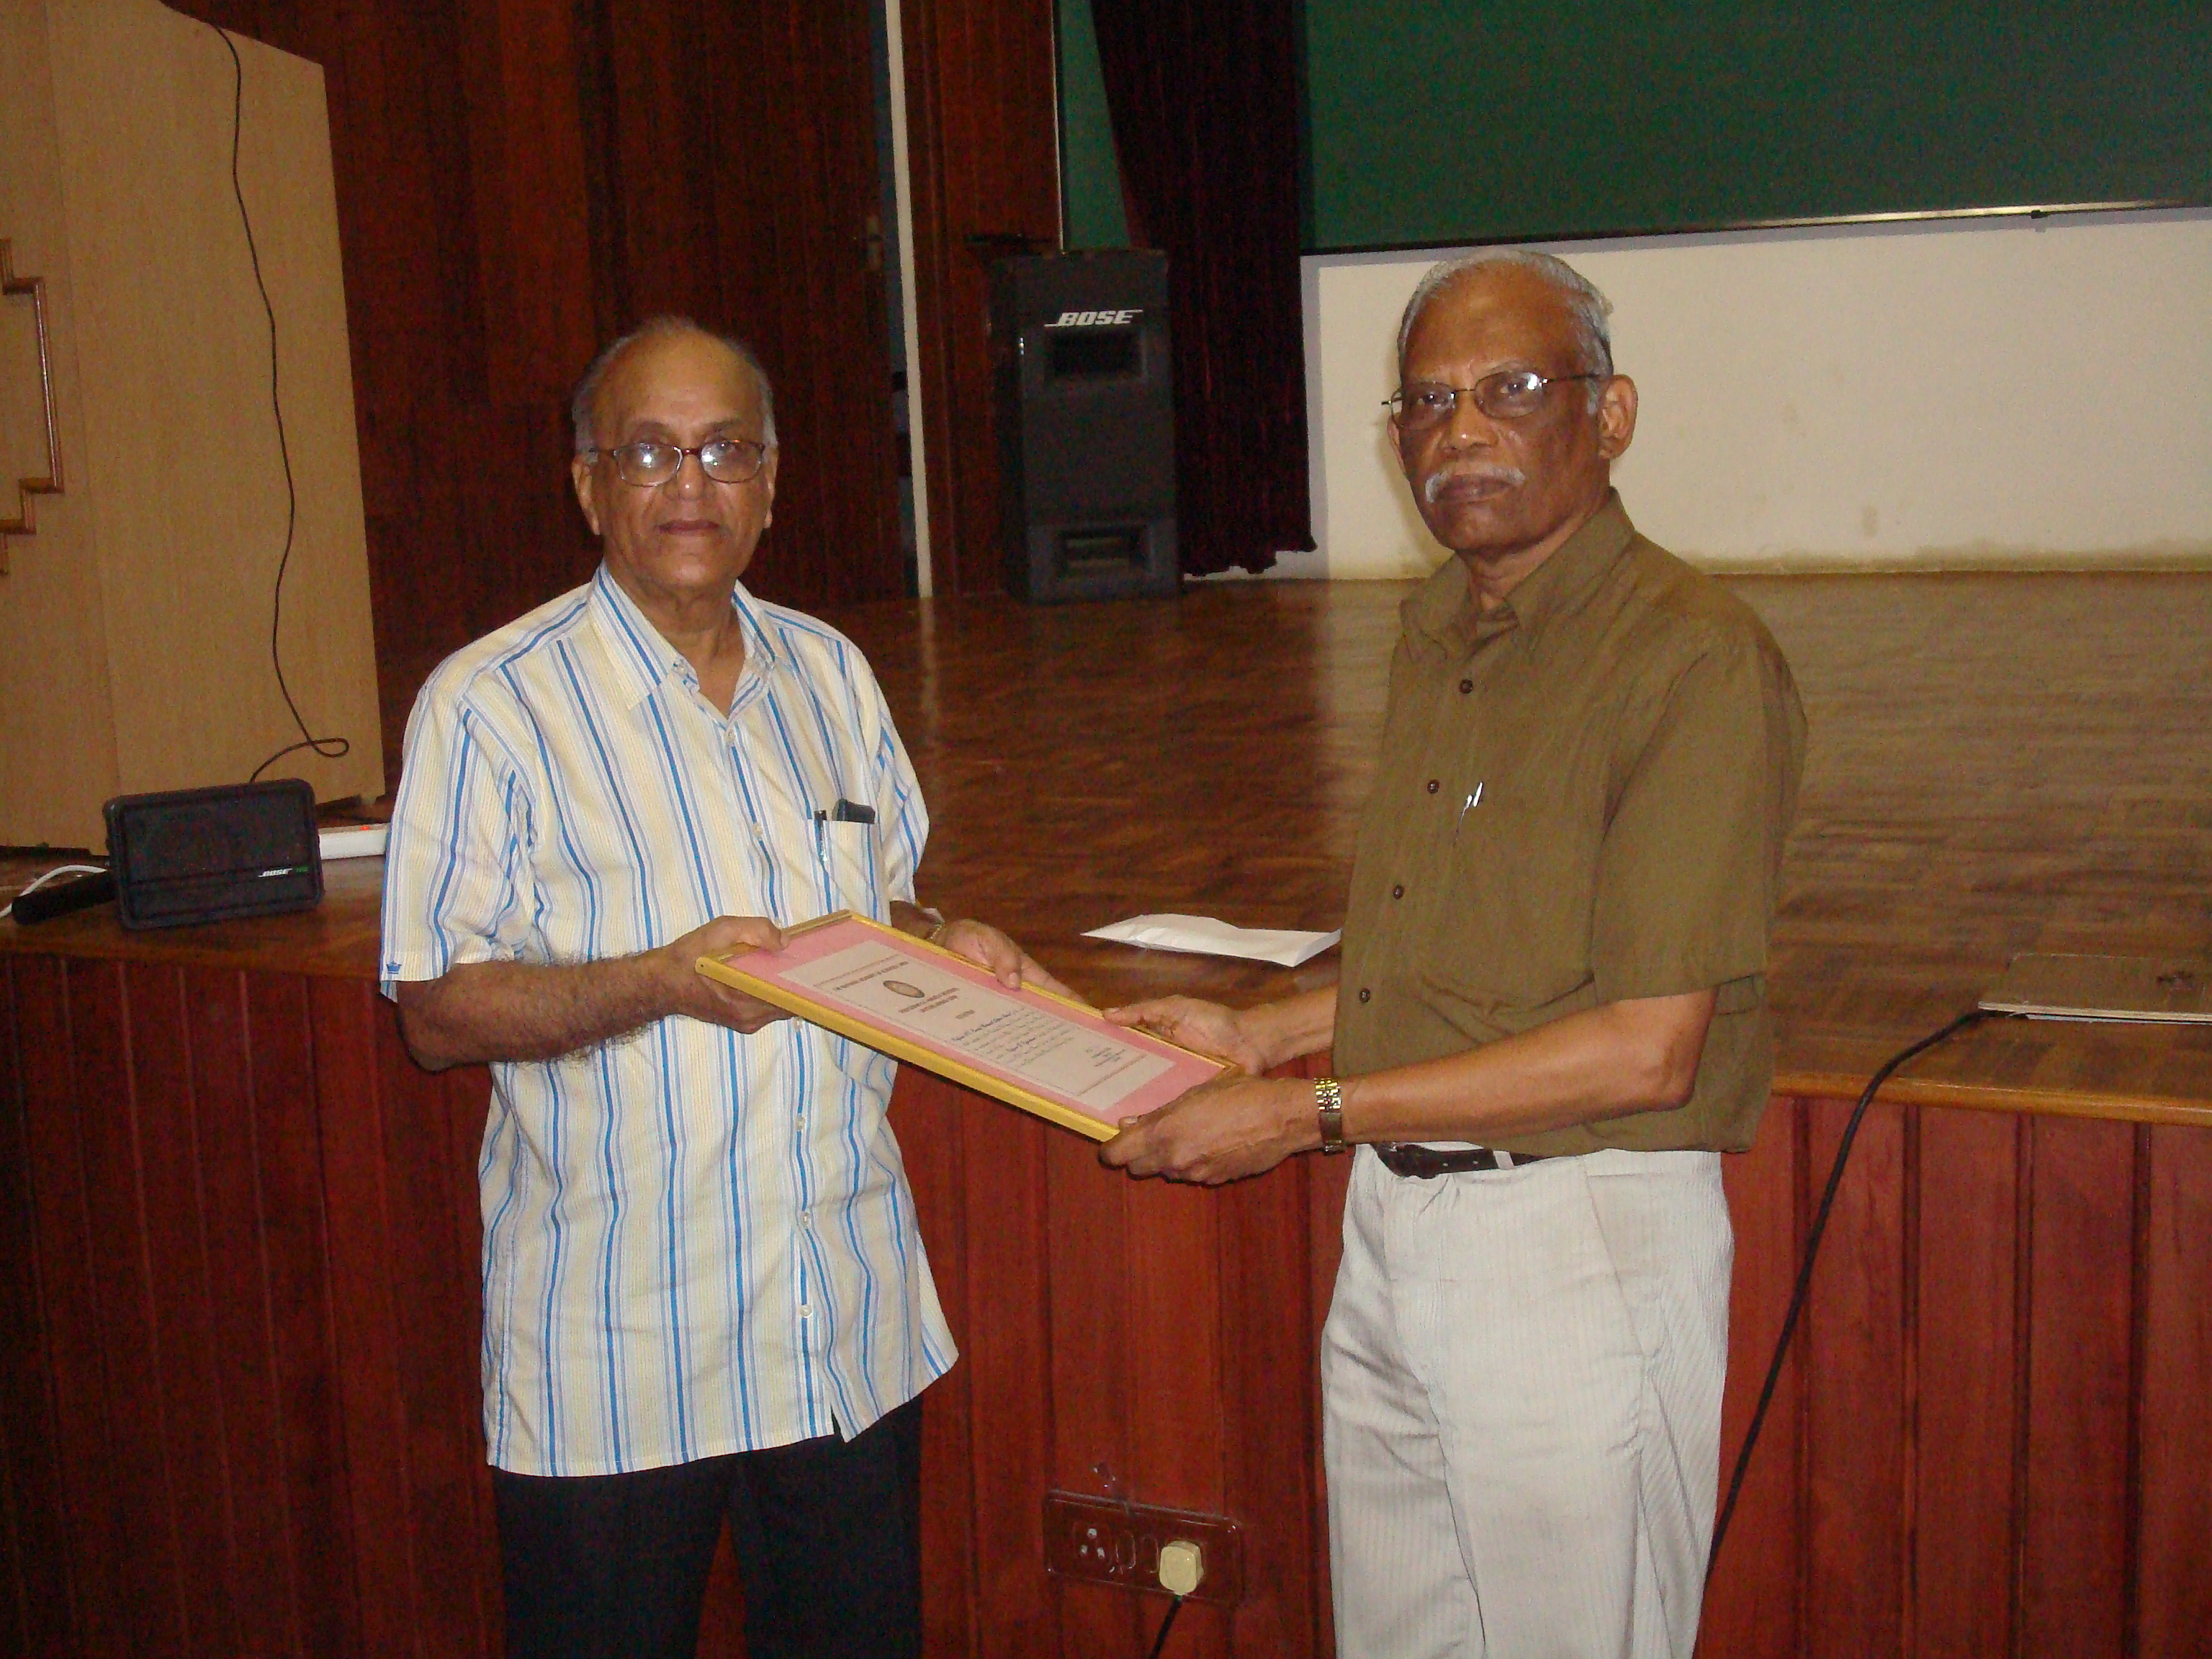
\includegraphics[width=0.7\textwidth]{Rajaji-seshadri.jpg}
\caption{Receiving the A C Banerjee Memorial Award of The
National Academy of Sciences from C S Seshadri, Director CMI.}
\end{figure}

Some of the other institutions in whose development I played a role as a 
member of their Governing Council or other bodies are Harishchandra 
Research Institute, Institute of Physics, Saha Institute of Nuclear 
Physics, Inter-University Centre for Astronomy and Astrophysics, SN Bose 
Centre for Basic Sciences, Indian Institute of Astrophysics and 
Astronomy and IISER, Thiruvananthapuram.

\section*{Teaching}

Apart from teaching full courses at CMI, I have been involved in 
considerable teaching in other Centres too. Academies-organized 
Refresher Courses in many Colleges in Tamil Nadu, Kerala and Karnataka 
took up a lot of my time and energy. For many of them I was the 
Director. Sunday Classes (venue: Dept of Nuclear Physics of the 
University) were started by Satyanarayana of Pondicherry University with 
the help of Joseph Prabagar of Loyola College. I joined the team and 
taught. I was involved in the running and teaching in the DST-organized 
SERC Schools in Theoretical High Energy Physics for more than ten years 
and I initiated the Physics Teaching for Talented Students. Courses in 
High Energy Physics were given by me at IISER-Thiruvananthapuram, 
IISER-Mohali, Banaras Hindu University Madurai Kamaraj University and 
many other institutions.
\begin{figure}[h]
\centering
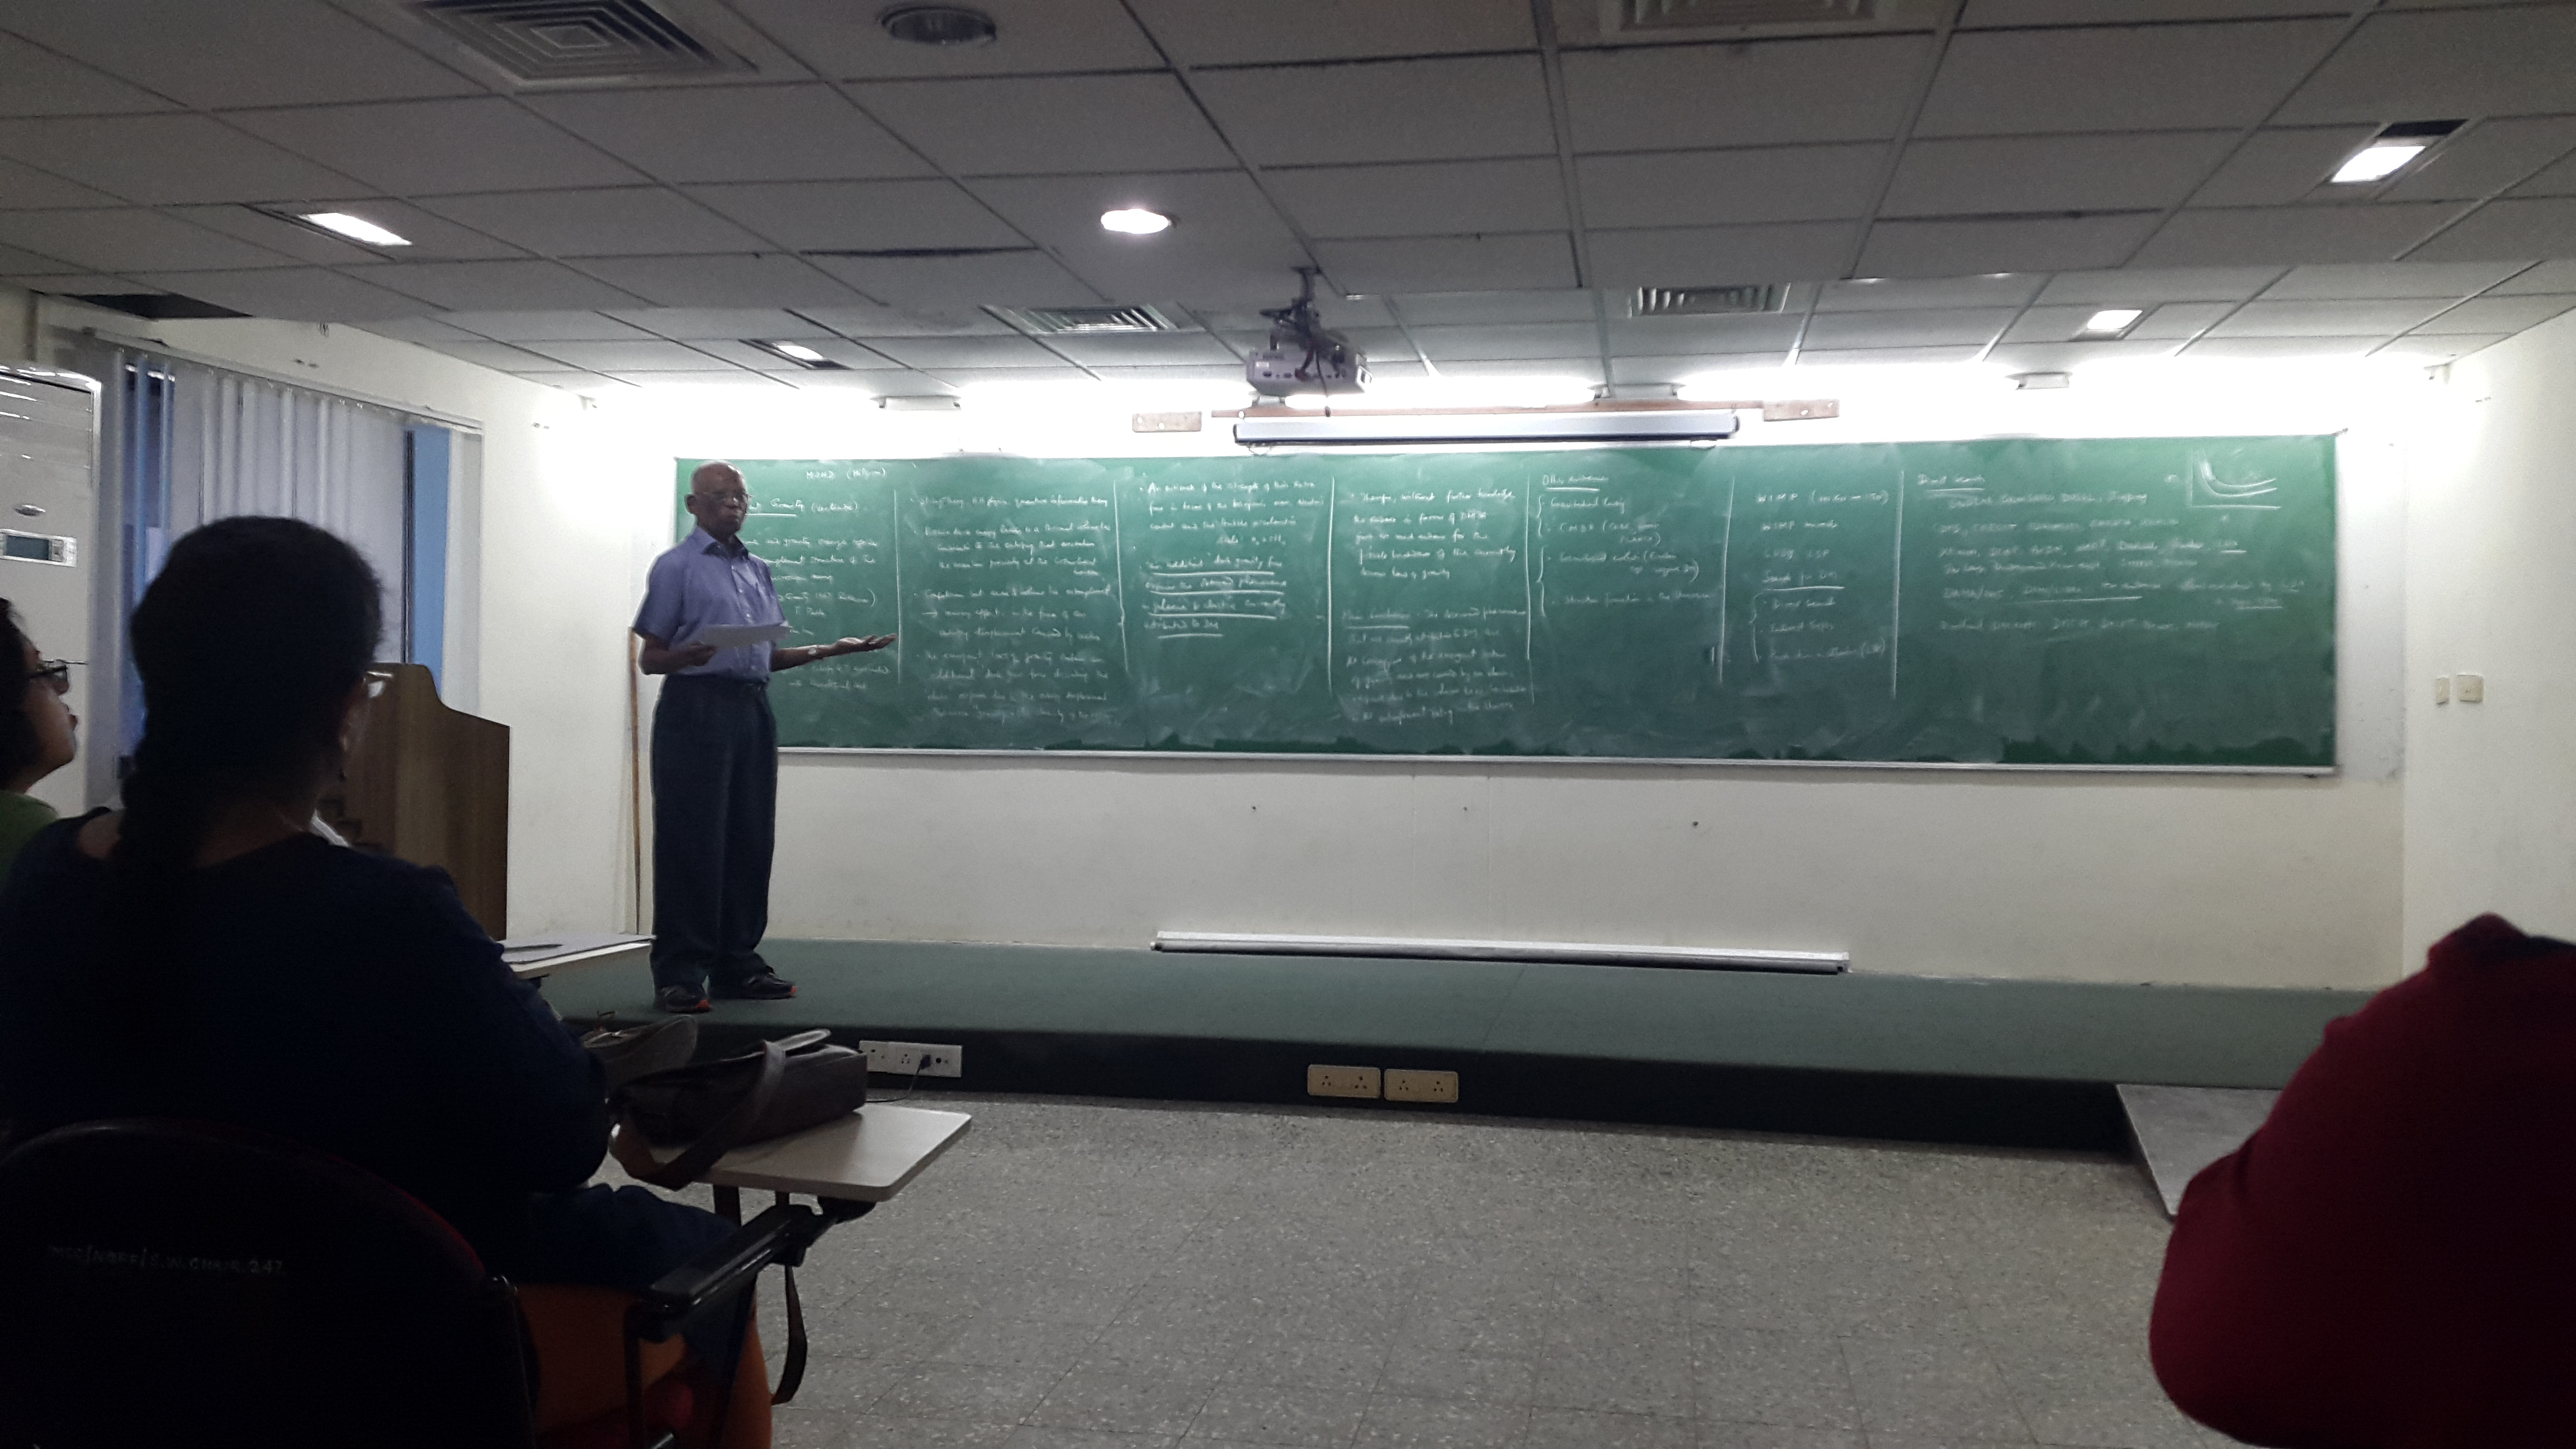
\includegraphics[width=\textwidth]{rajaji-teach1.jpg}
\caption{Lecturing at IMSc.}
\end{figure}

\section*{Popular Science}

I strongly believe that Popular Science will succeed in the country
only if it is done 
in the mother tongue of the people. My ambition to write Science in Tamil 
fructified through the kindness of my friend Dr Jeyapragasam who was the 
Editor of a Tamil monthly published from Madurai. I wrote every month 
and brought out two volumes containing my articles.
\begin{figure}[h]
\centering
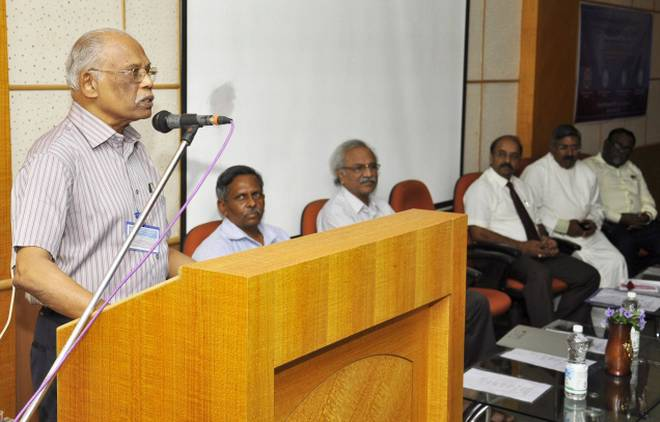
\includegraphics[width=\textwidth]{Rajaji-outreach-1.jpg}
\caption{At one of the Academy's Refresher School.}
\end{figure}
     
\section*{New Forms of Quantum Statistics}

AK Mishra and myself discovered many new forms of quantum statistics during
the period 1990 to 95. This was possible because of the Generalized Fock Space
that we constructed. Some of the new forms of statistics were Orthostatistics,
Null Statistics and Hubbard Statistics. Along with this we constructed many
new algebras of creation and destruction operators. Many of these are expected
to be used in future, in String Theory and other fundamental theories.

\section*{String Theory and LPA}

I was aware of String Theory almost from its birth. When I was perusing 
the preprint library in KEK, Japan in 1980 I saw the paper of Scherk and 
Shwartz who liberated String Theory from its hadronic context by 
changing the string tension from 1 GeV to $10^{19}$ GeV. That was the birth 
of String Theory. Then in 1984 I was escorting Tullio Regge from 
Bangalore to Madras and he told me the exciting discovery made by Green 
and Schwarz that all the anomalies cancel in the SO(32) and $E_8 \times E_8$ 
Superstring theories.

From then on I learnt whatever was known in String Theory and gave 
lectures on it in various Conferences, Workshops and the SERC School. 
But because of the heavy work involved in the building up of IMSc 
(1984-88) and the turmoil in 1989, I could not work in String Theory. 
But I kept up my interest in it because I believe that is the Theory for 
Future incorporating Standard Model and Quantum Gravity.

The main difficulty of String Theory is the lack of experimental 
support. That requires construction of accelerators going up to Planck 
energy $10^{19}$ GeV. Many regard that as impossible. This is a crisis in 
Physics. But human ingenuity knows no bounds and this energy barrier 
will be crossed. New principles of acceleration will be discovered. I 
have been emphasizing this for the last 40 years. Laser Plasma 
Acceleration (LPA) is one such and it has been pursued for some time all 
over the world. I have discussed the importance of starting LPA with 
experts on lasers at TIFR, Raja Ramanna Centre for Advanced Technology, 
Institute for Plasma Research and BARC. All of them met at the 
International Centre for Theoretical Sciences and they are chalking out 
a plan of action.

In the 80's I had many discussions with CVK Baba and MVN Murthy about 
building an accelerator of energy in the 5 to 10 GeV in India. DAE was 
willing to support it, but there was no enthusiasm among the 
experimental high energy physicists. They said such an accelerator would 
be useless unless it is more than 100 GeV. After this debate of ours, 
China built the Beijing storage ring of about 3 GeV which made many 
important contributions including a more precise measurement of tau mass 
which cleared many existing discrepancies.

Finally INDUS I and II were built after much delay but they were for 
synchrotron radiation.

Anyway, it is time that we now think of new methods of acceleration such 
as Laser Plasma Acceleration.


\section*{The contrast between the Indian situation pre-1971 and post-1984}

The success of the Standard Model based on YM theory has made YM a 
bandwagon. But I am talking about the pre-1971 era. As I already 
mentioned, I was lecturing on YM and electroweak theory in TIFR, SINP 
much before these things became popular, even before t'Hooft proved the 
renormalizability of YM with SBS. But there were no takers.

I remember, for instance, when I derived that in YM theory of weak and 
electromagnetic interactions the weak bosons have masses greater than 
37.4 GeV, many people jumped on my neck saying `` How can you put 
zero-mass photon and such heavy bosons in the same multiplet?". Times 
have changed. Now one routinely puts essentially ``zero-mass" particles 
and their superpartners, of TeV mass or even heavier, in the same 
supermultiplet.

When string theory came in 1984, there had arisen a sufficiently large 
number of capable young Indian physicists, both inside and outside the 
country who could pick up the new ideas fast and contribute at the front 
level.

It is clear that theoretical HEP in India has made rapid strides and now 
our theorists are equal to the best in the world.

\section*{Neutrinos}

Neutrino oscillations and neutrino mass were discovered during 
1996-2002. I was excited about Neutrino oscillations after I read about 
Mikheyev, Smirnow, Wolfenstein (MSW) effect in Bethe's PRL paper in 1986, 
that gave a beautiful explanation of MSW effect as a consequence of 
level crossing, during my visit to Hawaii in 1986. I conveyed that 
excitement to Anjan Joshipura and M V N Murthy who then wrote the first 
paper on three neutrino resonance phenomenon.

During the nineties,  MVN Murthy, D Indumathi, S Umasankar, 
Mohan Narayan and myself did considerable amount of work on neutrino 
phenomenology. We were the first to analyze all the neutrino data in a 
three-neutrino framework instead of the toy model using two neutrinos 
that was used until then. We were the first to analyze the null result 
of the CHOOSE reactor experiment on the basis of the three-neutrino 
framework and get an upper bound on the $\theta_{31}$ angle to be 12 degrees. 
Later experiments showed this angle to be 9 degrees, close to our upper 
bound.

I also worked on models of neutrino masses and mixing in collaboration 
with Ernest Ma of the University of California, Riverside. One of the 
models that we constructed, the $A_4$ model, became quite popular.

In collaboration with MK Parida and Rabi Mohapatra, I discovered the 
real reason for the neutrino mixing angles to be different from the 
quark mixing angles and so large. It is the renormalization group 
evolution. Both the leptonic and quark mixing angles are of the 
Wolfenstein form at high scale and the leptonic angles alone get 
magnified at low scale.
 
\section*{Raju Raghavan}

Raju Raghavan was a great experimental physicist. Although I knew him 
earlier since he was a second batch trainee, we became friends only 
after I came to Madras. He used to visit me whenever he came from USA 
and we discussed neutrinos. He had many original ideas on neutrino 
detection, including Mossbauer resonance absorption and emission of 
neutrinos. If one succeeds in this, neutrino experiments can be done on 
a table-top!
 
Later, after INO was conceived he was its enthusiastic promoter. He had 
conceived a detector of solar low energy neutrinos, called LENS (Low 
Energy Neutrino Spectrometer) which can revolutionize solar neutrino 
physics. He wanted to do the experiment in India. I took him to meet the 
secretaries of DAE and DST and they agreed to support him.

But Raghavan passed away suddenly in 2011. I was shocked and took a long 
time to recover. Actually at that moment when I heard the news, I was 
arranging a major meeting of Raghavan with scientists and science 
administrators. His death is a serious loss to Indian Science. India 
must take up the LENS Project.

\section*{India-based Neutrino Observatory (INO)}

India was a pioneer in neutrino experiments. The very first observation 
of cosmic ray produced neutrinos called atmospheric neutrinos was made 
in India, in the Kolar Gold Field (KGF) mines. That was in 1965. But the 
mines were closed in the 90's. Since there was not much gold, the 
Bharath Gold Mines company decided to close it. We should not have let 
that happen. ``Science is more precious than gold."

When the issue of possible closure of the KGF mines came up, I argued in 
favour of keeping them alive for future underground experiments. I 
raised it in many meetings. In the DST meeting on Thrust Areas held at 
Santiniketan, MVN Murthy presented both the issues, the case for keeping 
the KGF and construction of an accelerator for HEP.

It was neccessary to spend some money for keeping the water in the mines 
out by pumping. But that is negligible compared to the cost of digging 
new tunnels. If this had been done, there would have been a continuity 
in Indian neutrino experiments from Kolar to INO.

It is the atmospheric neutrinos which in the hands of the Japanese 
physicists enabled them to get two Nobel Prizes, in 1998 and 2002. We 
clearly missed the boat.

Can we recover this lost initiative? We can and we must. The INO was 
conceived with this aim in view.

It was conceived in IMSc in the year 2001, but it has not still seen the 
light. It was approved by all the Central Government bodies and the 
Government granted Rs 1600 crores for the project. This involves the 
construction of a 50,000 ton magnetised iron calorimeter detector for 
atmospheric neutrino studies. This will be installed inside a mountain 
in Theni District. The nerve-centre of INO will be in the outskirts of 
Madurai City and will house R and D of particle detectors with training 
facilities for students. This has been named Inter-Institutional Centre 
for High Energy Physics (IICHEP).
\begin{figure}[h]
\centering
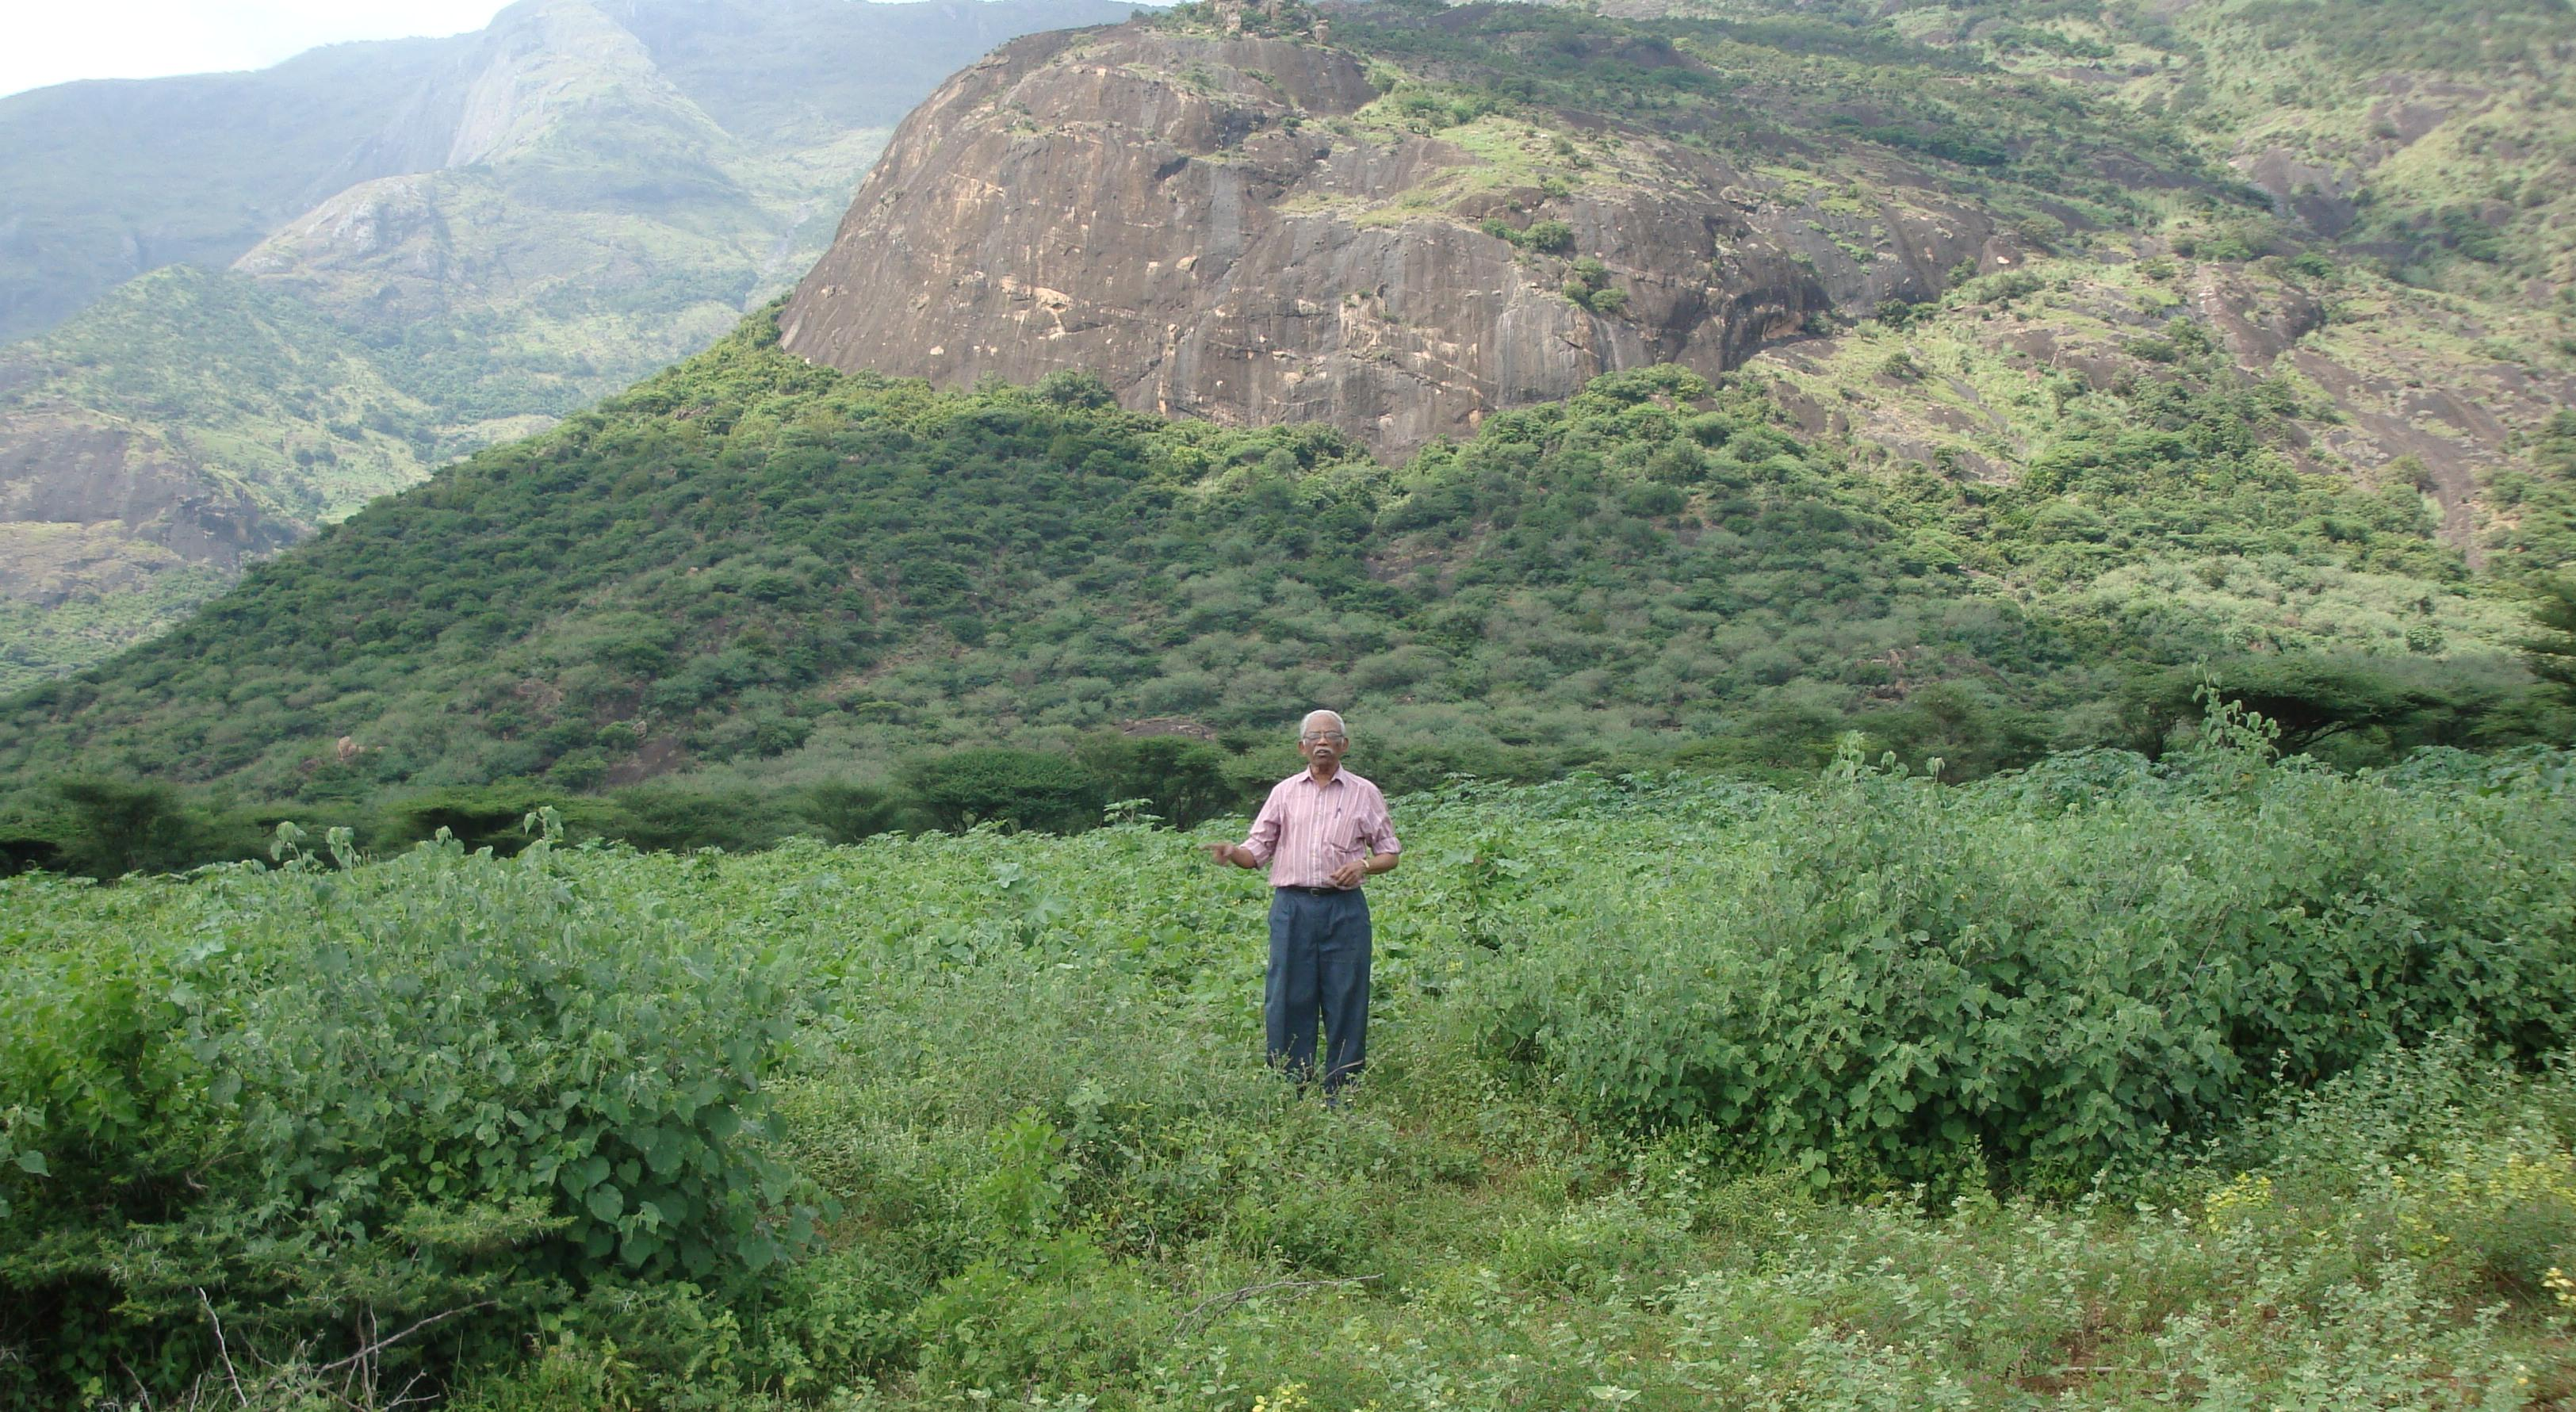
\includegraphics[width=\textwidth]{Rajaji-ino.jpg}
\caption{At the site in Theni District chosen for INO.}  
\end{figure}
Apart from the study of atmospheric neutrino oscillations, INO lab will 
house experiments searching for Neutrinoless Double Beta Decay (NDBD) 
and Dark Matter (DM). CVK Baba and myself played some role in initiating 
the NDBD activity. As a consequence two or three groups involving 
Vandana Nanal, RG Pillay, PK Raina and PK Rath are involved in 
feasibility studies for the NDBD project. I tried to initiate work on 
Dark Matter Search through Rupak Mohapatra of Texas A and M and 
physicists at SINP. This could have been a major project but it did not 
succeed. Instead a minor Dark Matter project at a shallow depth in the 
Jaduguda mines has been started.

Along with others I have lectured on INO to students in colleges and 
schools and villagers as a part of of the INO's outreach programme. This 
is continuing.
  
Some ``wise men" of Tamil Nadu blocked INO citing non-existent 
environmental and other imaginary dangers. This obscurantist propaganda 
must be fought and INO must succeed. Truth has to triumph.


\section*{Family}

I have been blessed with a loving family - Suthandra Devi (my wife), 
Poongodhai and Uma (my daughters), Sunil Ramachandran (Poongodhai's 
husband), James Harano, (Uma's husband), Anjali and Shalini 
(Poongodhai's daughters) and Kailash (Uma's son).
Along with my family there are many friends who supported me, too 
numerous to mention by name.

\begin{figure}[h]
\centering
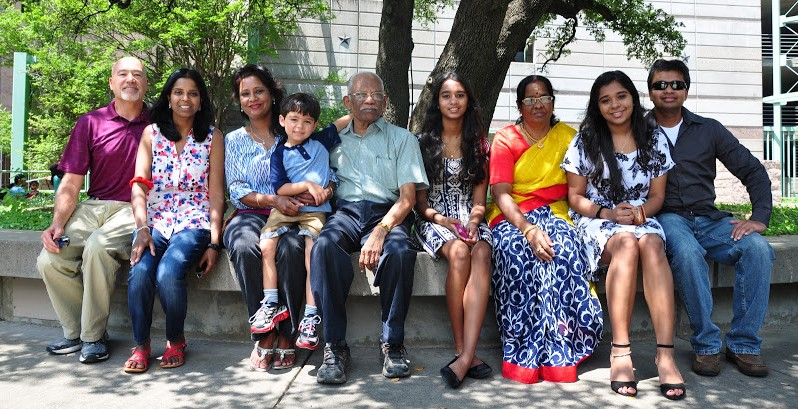
\includegraphics[width=1.1\textwidth]{Rajaji-family-1.jpg}
\caption{Circa 2017 L to R: James, Uma, Poongodhai, Kailash, GR,
Shalini, Suthandra, Anjali, Sunil.}
\end{figure}

\newpage
~

\newpage
\thispagestyle{empty}
~
\vfill
{\centering{\Huge\bf{Part II: My Scientific Autobiography}}}
\vfill
~
\newpage
~
\chapter*{My Scientific Autobiography}

\paragraph{The Beginning}:

A crucial event occured when I was in the Intermediate class of the 
Amercan College, Madurai. A friend of mine took me to observe the night 
sky through the College telescope.

It was the best time to observe the Moon since the shadows of the 
mountains were long. When I saw the deep craters and high mountains, it 
was as if I was looking down at the Moon from a height. It was a 
frightening sight. I realized that

There are more things in heaven and earth than are dreamt of in my 
philosophy.

Science is the key to these other things and that determined my 
trajectory in life.

\paragraph{Preparation}:

I joined TIFR in August 1958 after one year in the AEET(BARC,now) 
Training School.  Since my mind was bent on understanding physics at its 
most fundamental level, I first took up the study of Quantum Mechanics, 
since my knowledge of it was not strong. For any question that I asked, 
the answer was in Quantum Mechanics. I sat with LI Schiff's book on 
Quantum Mechanics for many months and mastered it.

Then I turned to Nuclear Physics since that was the most fundamental 
subject at that time. I read Bethe and Morrison and then Blatt and 
Weisskopf. Went to Kailash Kumar and George Abraham for guidance. The 
former put me in contact with many body theory and the latter in contact 
with few body problems. Abraham even suggested a specific problem. He 
asked me to redo the deuteron and triton structure using the recently 
discovered hard-core repulsion between nucleons.

I was not satisfied. I realized that the force between the nucleons 
comes from a deeper layer of reality which can be understood only from 
the then-new area called particle physics. There was no particle physics 
research in TIFR at that time. B M Udgaonkar (BMU) started studying 
hepernuclei which was in between nuclear and particle physics. 
Hepernuclei are nuclei in which one nucleon is replaced by a lambda 
particle. He introduced me to this subject and also to a few excellent 
reviews by Enrico Fermi on quantum theory of radiation and isospin 
symmetry. Udgaonkar was an excellent teacher. He had taught our batch of 
trainees reactor physics and the second batch quantum mechanics. Bhabha 
had sent him to France to learn about reactors, but BMU shifted to 
particle physics after returning.

Soon SN Biswas and LK Pandit joined and real particle physics started in 
the Theory Group. I started reading particle physics and learnt that the 
real theory of particle physics was Quantum Field Theory (QFT). So 
finally I reached the destination of my "Inward Bound" journey.

I took up Bethe and Schweber's QFT and Jauch and Rohrlich's Theory of 
Photons and Electrons. I really loved the systematic treatment of QFT in 
Wentzel's book. I took it during my vacation in Kamuthi and read it even 
during the long train journeys.

My learning of QFT was systematized and consolidated only after I 
listened to LK Pandit's course of lectures on QFT. I was so impressed by 
his excellent lectures that I felt I achieved "Enlightenment".

Soon I began to interact with Biswas.

I will divide the account of my work into two parts; Pre-Standard Model 
and Post-Standard Model. The numbers here refer to the list of 
publications at the end.

\section*{Pre-Standard Model}

This can be subdivided into three parts, Hypernuclear Physics,
SU(3) and Hadronic Resonances and Current Algebra.

\paragraph{Hypernuclear Physics}:

My first paper [1] was in this field. I had learnt hypernuclear physics 
from BM Udgankar and RH Dalitz's papers. After listening to SN Biswas's 
excellent lectures on integral equations I was impressed by the fact 
that integral equations can be easily solved if the kernel is separable. 
Using this, with SN Biswas's collaboration I could solve the two-channel 
problem of Lambda-Nucleon scattering. We applied it to Gell-Mann's 
global symmetry and proved that global symmetry that equated all the 
meson-baryon coupling constants does not work.

The next two papers [2,4] were in collaboration with Dalitz in Chicago. 
The first was on the lifetime of the light hypernuclei such as 
Lambda-$H^3$. The binding here is so weak that the life time is not 
expected to be very different from the lifetime of the free Lambda. 
Experiments did not agree with this. This discrepancy exists even now 
and the problem is not yet solved!

The second paper on hypernuclear physics was on the binding of 
Lambda-Lambda hypernuclei. Here we had to do a three-body problem. We 
did a variational calculation with many parameters in the wave function. 
It was done using the new IBM computer in Chicago University. One 
punches the Fortran programme on cards and submits it. After several 
hours you are informed of the error in punching. You repeat the process. 
Finally I succeeded and the paper was written.

\paragraph{SU(3) and hadronic resonances}:

At that time the dominant school of thought was the S matrix philosophy 
of GF Chew. Proving Mandelstam's double dispersion relations was 
considered the biggest challenge. Reinhard Oehme lectured to us on the 
many-sheeted S matrix.

AP Balachandran who had already obtained his PhD in Madras and joined as 
Dalitz's post-doc was frightening students like me by talking about the 
theory of many complex variables and "The Edge of the Wedge Theorem". He 
was very mathematically oriented.

Those days you either group or disperse. The former led to SU(3) group 
and the later led to Dispersion Relations. An interesting story about 
the proof of Dispersion Relations from Field Theory is the following:

Feynman: What is Dispersion Relation?

Wigner: What is Field Theory?

Chew: What is Proof?

I had mentioned to Dalitz that I would like to work on a problem nearer 
to the core of Particle Physics. Dalitz agreed and gave me a recent 
preprint from RJ Oakes and CN Yang that had arrived. They had criticized 
Gell-Mann's SU(3) on two counts:

1.The mass differences in the baryonic octet and the same in the mesonic 
octet being very large, the decimet baryons Delta (1238), Sigma (1370), 
cascade (1520) and $\Omega^-$(1670) occur as poles on different Riemann 
sheets. So there is no way in which they can move smoothly to emerge as 
a single pole in the SU(3) limit.

2. Because of the large mass differences again, there is no way by which 
the perturbative Gell-Mann-Okubo mass formula can work.

Since I had learnt about the various Riemann sheets of the S matrix from 
Oehme's papers, I could answer the first objection: there is a retinue 
of poles residing in all the Riemann sheets. These were subsequently 
called "shadow poles". Because of the existence of shadow poles, one of 
the tenets of S Matrix theory which defines a particle as a pole of the 
S matrix must be modified. The whole retinue of poles define the 
particle!

Any typical American physicist would have sent this to the Physical 
Review Letters immediately. Dalitz is more conservative and we sent a 
letter to Oakes and Yang and both of us left for Oxford! Meanwhile many 
others published this result. Later our delayed publications came out 
[3,5]. The second objection can be answered only by detailed 
calculations and that became my thesis[6]. I showed that if the momentum 
is small compared to the inverse of the range of the interaction, 
perturbation theory is valid.

Dalitz, TC Wong amd myself wrote a paper [7] on the hadron Lambda 
(1405). We used a relativistic mutichannel version of Schrodinger 
equation with potential arising from exchange of rho and omega and could 
generate Lambda (1405).

When I returned to Bombay I began thinking about this problem. By that 
time quark model had come up. The question was: is Lambda (1405) a bound 
state of three quarks or is it a composite of a baryon and a meson? I 
discovered a way of answering this question.

I showed that the hadron Lambda (1405) cannot be a three-quark bound 
state, but it is a composite of a baryon and meson, the so-called 
"molecular hadron". The test was simply that if it were a quark 
composite, the K matrix for meson-baryon scattering must have a pole but 
such a pole did not exist for K bar-N, pi-Sigma scattering. I talked 
about this result in two conferences, HEP Symposium at Aligarh [10] and 
Matscience Symposium [13],but did not publish in any journal.

I learnt from my friend Sandip Pakvasa that my teacher Dalitz was not 
happy with me. Since earlier Dalitz, Wong and myself had worked on this 
hadron, perhaps he felt that he should be a coauthor in the K-pole 
paper. I wrote to him apologizing for what I did and explaining the 
circumstances in which this happened. Then I wrote a detailed paper in 
Physical Review [24] making due references to Dalitz's work and also 
thanking him. This paper contains a possible extension of the K pole 
text to many other hadrons too.

Much later after QCD came up, it was shown in the paper Phys Rev Let, 
114, 132002 (2015) that QCD also supports the conclusion that Lambda 
(1405) is not a three-quark bound state.

In [8] I showed that in contrast to Lambda (1405) the decimet baryons 
cannot be meson-baryon composites, thus showing that the prevalent 
S-matrix bootstrap philosophy was wrong. With SS Vasan I showed the 
stability of the S matrix pole under various paramatrizations of the 
scattering amplitude.
 
\paragraph{Current Algebra, K decays etc}:

During 69-71, current algebra became the main focus. I wrote a few 
papers connected to Schwinger terms in collaboration with V Gupta 
[15,16,20]. This led to the discovery of a fixed pole in virtual Compton 
amplitude [21]. This paper has an interesting history. Rajaraman and 
Sudendhu Roy Chowdhuri had sent out a preprint pointing out a 
discrepancy between a theoretical sum rule and data on deep inelastic 
electron-nucleon scattering data. I could immediately see that they had 
ignored a possible fixed pole which is indicated by our earlier work on 
Schwinger term in Current Algebra. I pointed this out to Rajaraman who 
was visiting TIFR. On his return to Delhi he corrected the preprint and 
published it with SR Choudhury. But they did not acknowledge me for 
pointing out their error!

I reviewed [11] an important paper of Abers, Dicus and Norton who 
derived the radiative correcton to beta decay using Current Algebra.

The paper [17] was written with KVL Sarma and it addressed the question 
of electron-muon universality in K decays. This is a recurrent topic and 
right now this family universality is an important topic in B decays. 
Papers [18],[19] and [23] written in collaboration with a student SC 
Chhajlani and LK Pandit applied Current Algebra to K decays.

With PP Divakaran and V Gupta I studied the question whether the 
electromagnetic current could have an I = 2 component [12]. The paper 
[27] with PP Divakaran connected the form of the deep inelastic 
structure function with the asymototic behavior of the elastic form 
factor.

\section*{Post-Standard Model}

\paragraph{Gauge Theory}:

I became aware of Yang-Mills (YM) theory by reading J J Sakurai's paper 
in Annals of Physics in 1959. That was the first paper in which YM was 
used in particle physics. Sakurai constructed a gauge theory of strong 
interactions. I continued to be interested in YM theory from that time. 
Veltman's lecture at Varenna where he talked about the conserved weak 
current impressed me very much and I felt that weak interaction must be 
described by a YM theory. So, when Weinberg's paper on the SU(2)xU(1) 
electroweak theory came out in 1967 I had no doubt that was the correct 
theory. I read the papers of Goldstone, Higgs and Kibble.

In the subsequent two or three years, I lectured on these at various 
places including TIFR. In particular, in June 1971, I gave a series of 
lectures on the gauge theory of weak interactions including Yang-Mills 
theory, Faddeev-Popov ghosts, Higgs mechanism, electroweak theory, GIM 
mechanism etc. It came out as a SINP report [25]. This was the first 
connected account of what became known as the Standard Model, anywhere 
in the world! It even contained my conjecture that the massless YM gauge 
quantum cannot exist as a particle because of the incurable infrared 
divergences (an early suggestion of what became known later as infrared 
slavery and colour confinement). These lectures were given even before 
t'Hooft's proof of renormalizability appeared!

Nevertheless I failed to make any substantial contribution in gauge 
theory. I will not go over the reasons here.

Then came the discovery of asymtotic freedom of YM theory by Gross, 
Wilczek and Politzer and the construction of SU(3) colour gauge theory 
by Gell-mann, Fritzche and Leutwyler to describe strong interactions.

Renormalizabily of YM with SSB and Asymptotic Freedom are the two most 
important discoveries in Quantum Fild Theory after the discovery of 
renormalizability of Quantum Electrodynamics in 1947-49. I missed the 
boat in both, although I was well-placed with potential to contribute. I 
had already studied path integrals which t'Hooft used in his proof and 
was already giving lectures on Wilson's Renormalization Group and 
Callan-Symanzig equations which are the ingredients in the discovery of 
asymtotic freedom by Politzer, Gross and Wilczek.

Although I missed the stage, I was sitting in the front row. I could 
catch their significance as soon as the discoveries came tumbling one 
after another! The years 1971-73 were truly exiting years. It was the 
watershed in the development of High Energy Physics.

In [26], I showed that divergences in the higher-order corrections 
calculated in the SU(2)xU(1) theory cancel.

In the First Symposium on HEP at Bombay in 1972, I reviewed the 
electroweak theory [29]. This was the first review of the electroweak 
theory in the country.
 
Actually, until t'Hooft's proof, as far as I know, nobody except Joe 
Schechter in Syracuse University who added a U(1) to cancel the 
strangeness-changing neutral current and myself had taken Weinberg's 
theory seriously. Even after t'Hooft, only a few theorists took it 
seriously. Situation changed dramatically after the discovery of the 
weak neutral current interaction in the CERN experiment by Perkins and 
others in 1973.

In 1969, TIFR's theoretical physics summer school was held at Nainital. 
Some memorable events took place there. Both Geoffrey Chew and Francis 
Low lectured. Chew lectured on S Matrix Theory. I asked him a question: 
Since S Matrix theory addressed only strong interactions, what happens 
to weak and electromagnetic interactions? Chew gazed at the distant 
Himalayan peaks visible through the window for a few minutes and simply 
continued his lecture.

Low lectured on the divergence problem of the Fermi theory of weak 
interaction and described all the methods proposed to deal with the 
problem. This was two years after Weinberg's paper. I asked Low at the 
end of his lectures why was he ignoring the Yang-Mills theory of weak 
interactions. He merely stared at me and refused to answer my question. 
He described seven or eight unnatural ways of solving the weak 
interaction problem but left out the one way that turned out to be the 
right way. To this day I have not understood how such a thing is 
possible, Low being a very experienced physicist. Somebody said it was 
because Low did not like Weinberg! Tapas Das and myself took notes of 
Low's lectures and brought it out as a TIFR yellow report.

The evolution of the name starting from Gauge Theory is interesting. As 
soon as t'Hooft showed the renormalizability of electroweak theory I 
calculated the radiative correction to muon decay and sent it to 
Physical Review for publication[26]. I had put the title as "Radiative 
correction to the muon decay in gauge theory". Physical Review changed 
it to "Weinberg's gauge theory". In 1972 the HEP Conference was held at 
Chicago that I attended. That is where gauge theory was presented as a 
Rapporteur's talk for the first time. BW Lee gave the talk. He called 
the theory as "Salam-Weinberg gauge theory". Salam and Gell-Mann were 
sitting in the first row and I happended to be sitting in the second row 
just behind Salam and Gell-Mann. As soon as Lee mentioned 
"Salam-Weinberg gauge theory", Gell-Mann gave a nudge to Salam with his 
elbow. Later when the Nobel Prize was given, Glashow's name was added 
and the theory became Glashow-Salam-Gell-Mann theory. This is certainly 
justified since Glashow was the first to discover that SU(2)xU(1) was 
the correct gauge group for electroweak theory and also he was one of 
the inventors of the Glashow-Iliopoulos-Maiani (GIM) mechanism to remove 
the strangeness changing neutral current.

However I prefer to call it the SU(2) x U(1) Electroweak Theory.

\paragraph{Neutral Current}:

Weak neutral current (NC) interaction is almost as strong as the usual 
charged current (CC) weak interaction but lay undiscovered all those 
years. It could have been discovered many years earlier if only the 
experimenters did not listen to some theorists who said NC cannot exist. 
The theorists thought that NC would lead to strangeness changing NC 
decays which were not seen, but they forgot that there could be 
strangeness nonchanging NC. So the experimenters ignored some data which 
were actually due to NC. But the clinching experimental proof was 
possible only after the huge Gargamelle bubble chamber was constructed 
at CERN. Because of its size they could clearly distinguish a pion from 
muon and this was crucial for the discovery of NC through the absence of 
muon in neutrino collision.

As soon as the discovery of NC was announced, KVL Sarma and myself 
produced the first model-independant analysis of deep inelastic data 
[30,32,33]. JJ Sakurai called our equations "Master Equations". His 
analysis of elastic scattering using the master equations coupled with 
LM Sehgal's of single pion production led to the complete determination 
of NC coupling constants. Later with Sandip Pakvasa, I generalized the 
analysis to include S,P and T neutral current interactions. With KVL 
Sarma I wrote two more papers on this topic [44,52]. With SH Patil I 
calculated the contribution of neutral current to the decay $K_L \rightarrow
\mu^+ + \mu^-$ [28].

\paragraph{Integrally charged quarks}:

Our work on Integrally Charged Quarks (ICQ) has a curious history. While 
working on the neutral current paper [35] with Pakvasa, I noticed that 
if there are charged spin one partons, deep inelastic structure 
functions will not scale. Probir Roy and myself pointed this out for the 
neutral current [37]. We noticed that scaling will be restored in a 
unified gauge model. This is how we arrived at the Han-Nambu model which 
we gauged. The results were remarkable:

1. Although the Han-Nambu quarks are integrally charged, as observed 
through high $q^2$ probes, they behave like the Gell-Mann-Zweig 
fractionally charged quarks (FCQ).

2. Gluons acquire electrical charge and have weak interactions also.

Papers [40,42] are on this work. I derived these results in a somewhat 
more general way in [43].

Soon we saw a preprint by JC Pati and Abdus Salam who also had the same 
model with ICQ. But they did not notice the second result, namely the 
gluons have electrical charge. We pointed this out to them in a letter 
and immediately, Salam sent a cable "We were wrong and you are right." 
They also corrected the published version of their preprint. But they 
did not refer to our work at all!

After I joined Madras University I worked with my collaborators 
S~D~Rindani, T Jayaraman and S Lakshmibala and confronted the ICQ model with 
experiments on deep inelastic scattering and electron-positron 
annihilation and also analyzed other consequences of the model 
[54,61,63,64,65,66,70,71,78,79,82,83,86,87,88,98]. In some of these 
papers there were other collaborators: HS Mani, R Godbole, JC Pati, X.-G 
He, S Pakvasa, and NG Deshpande. To this day, the ICQ model has not been 
disproved.

Some of the other works on the broken colour model are [70],[98].

In an important paper [81] with T Jayaraman and SD Rindani it was shown 
that the time- honoured Equivalent Photon Approximation does not work 
for massive spin-1 charged particles unless modified suitably. This was 
inspired by our work on ICQ model.

Some time ago, I noticed that the model with broken colour solves the 
problem of strong CP violation from which the standard QCD suffers. I 
have not yet published this result.

\paragraph{How I proved three Nobel Laureates wrong!}:

1. Our discovery of shadow poles in disproving CN Yang's objection to 
SU(3) has been already described.

2. The discovery of CP violation in 1964 by Cronin and Fitch created 
quite a lot of excitement. V Gupta returned to TIFR after a stay at 
Caltech and he showed me a Phys Rev Lett paper in which he had proposed 
what looked like a very elegant model of CP violation. He had discussed 
this with Gell-Mann. I spotted a big error that Gell-Mann did not 
notice! This model violated CPT theorem and hence is untenable!This 
paper [9] is the shotest paper I ever published.

3. While working on ICQ model, we showed Salam was wrong. This is 
described above.

I have to balance the above by the following.

\paragraph{My failed attempts}:

1.This was soon after I joined TIFR in 1958. In the primordial nucleo 
synthesis there was a gap. In the successive cooking of nuclei starting 
from proton by abrorption of a neutron, there seemed to be a gap at A = 
5. Because $He^5$ is not bound. When I learnt that the hypernucleus 
Lambda-$He^5$ is bound, I thought that is the solution. I discussed it 
with Udgaonkar, but it did not work.

2.After CP violation was discovered from K decays into two pions in 
1964, I thought the ugly CP violation can be avoided by recognizing that 
since pions are quark-antiquark bound states, Bose statistics for pions 
is only approximately valid and without Bose statistics, CP violation 
cannot be inferred. This idea too did not work.

3.During 1964-64, with Arvind Kumar who joined me as a student, I 
undertook a massive calculation aiming to construct a complete theory of 
hypernuclei. Infact Arvind Kumar managed to do an enormous amount of 
calculation. It did not lead anywhere.

4.I tried to generate the nucleon-pion coupling using the quarks of 
which N and pi were made. This also did not lead anywhere.

5.For quite a long time,I imagined quarks to be leptons. That would have 
been the natural explanation for quarks and leptons satisfying the same 
current algebra. I tried to construct a mechanism by which the weakly 
interacting leptons could sometimes exhibit strong interactions, but I 
failed.

6. During 1967-70, I tried to construct strong interactions from weak 
interactions. by using the divergences of Fermi's weak interaction 
theory. TD Lee had shown how the quadratic divergences could be turned 
to strong interactions. Gell-Mann, Goldberger, Kroll and Karplus wrote a 
nice paper showing how the quadratic divergences in the diagonal parity 
and strangeness conserving sector could be identified as the strong 
interactions. My aim was to redo these calculations using the YM theory 
of weak interactions of Weinberg's 1967 paper. But alas! t'Hooft proved 
the renormalizability of Weinberg's theory. No divergences were left to 
generate strong interactions!

\paragraph{Psi particle}:

In 1974 I was invited by my friend Sandip Pakvasa to visit the 
University of Hawaii, Honolulu. Sandip and myself worked on the paper 
[35]. Since I had gone with my family, I wanted to show them Hawaii. But 
in October of that year all hell broke loose! A very narrow peak at 3.1 
GeV was seen in electron-positron collisions. San Fu Tuan was constantly 
at the phone pumping out information on the new discovery from Stanford 
and other Centres. We wrote up a dozen explanations[34]. Fortunately it 
included the correct explanation: it was a bound state of the new 
charmed quark and a charmed antiquark. Papers [36,39,41] on the charmed 
particles were written in collaboration with J Pasupathy and KVL Sarma.

\paragraph{Madras University}:

In 1976 I shifted to University of Madras. I was very much worried since 
this happened when I was at the peak of my career and feared that my 
academic performance will be afftected. Fortunately this did not happen, 
mainly because of a brilliant physicist V Srinivasan. Using functional 
methods, Srinivasan and myself could show the equivalence of many field 
theories. In particu;ar we could show the equivalence of Parisi's model 
of quark confinement with QCD! [46,47,48,49,80] are the papers written 
in collaboration with Srinivasan; in the last paper MS Sriram also was a 
coauthor.

Soon SD Rindani joined as a faculty member and Sriram and JK Bajaj 
joined as Research Associates under my UGC project "Gauge Theory". Under 
the enlightened leadership of the Vice Chancellor Malcolm Adiseshaiah, 
MSc teaching started. Two good MSc students T Jayaraman and S 
Lakshmibala joined me for PhD. So we had built up an active Theory group 
in the University.

\section*{Activities in IMSc Phase}

\paragraph{Quantum Statistics}:

After I rejoined Institute of Mathematical Sciences after one year at 
TIFR, AK Mishra joined IMSc. He is very good at long algebraic 
calculations. One day he came to my office and showed me a new algebra 
of creation and destruction operators. He constructed this while 
studying Hubbard model where the Coulomb interaction between electrons 
at the same site is so large that only one electron is allowed at one 
site. This was the starting point of our long and fruitful 
collaboration. We constructed a Generalized Fock Space which allowed us 
to discover many new forms of quantum statistics [115]. These were 
Orthostatistics, Null Statistics, Hubbard Statistics and many others 
[102,106,107,108, 108,116,111,112,113,118,120,123]. Some related work 
with AK Mishra, A Khare and RP Malik was published in [107,108,127].

\paragraph{Neutrinos}:

Neutrino Physics came to centre stage after the discovery of neutrino 
oscillations. Most people worked on the toy model of oscillations with 
two neutrinos. The Madras group was one of the earliest to work with the 
full three-neutrino oscillations. In [121] and [122] I worked on solar 
and atmospheric neutrino oscillations with MVN Murthy, S Uma Sankar and 
Mohan Narayan. We were the first to give the correct interpreation of 
the null result that came from the CHOOSE reactor experiment [132]. We 
could give an upper bound on the reactor mixing angle $\theta_{12}$. This 
upper bound of 11 degrees was the only information on this mixing angle 
until Daya Bay experiment determined it to be about 9 degrees, not 
far away from our upper bound.

Actually the CHOOSE preprint concluded wrongly that their result 
contradicts the earlier experimental result on atmospheric neutrinos. 
This was because they used the wrong toy model of two neutrinos. The 
published version removed this statement since we had written to them, 
but they did not refer to us at all!"

Since we had an analytical way of doing neutrino propagation in matter, 
Rahul Sinha, Mohan Narayan and myself could do many calculations more 
easily. We could calculate in detail the time-of-night variation of 
solar neutrinos during their passage through the Earth [125]. In 
collaboration with C Burgess we could calculate the Eclipse Effect in 
which neutrinos get regenerated during their passage through the Moon 
[124, 126]. So, as observed through a neutrino telescope, the Sun 
appears brighter during the eclipse!

I worked on neutrinos from Supernovae in collboration with MVN Murthy, D 
Indumathi and G Dutta.[135,140,143]

Most of this work was reviewed in [130].

Using RG evolution we showed how the neutrino mixing angles which are 
small at high scales evolve to become large at small scales and match 
the experimental values [151,156,158,164]. My collaborators were RN 
Mohapatra, and MK Parida and later SK Agarwalla. In collaboration with G 
Abbas, S Gupta, R Srivastava, MZ Abyaneh and M Patra these calculations 
were pursued with updated input and in one paper,replacing Majorana with 
Dirac neutrions [181,182,185].

In all the above RG work, the neutrino mixing angles were taken to be 
equal to the quark mixing angles at high scale under the assumption of 
lepton-quark unification. Later I realized that this unification 
hypothesis was unneccessary. What was needed was the Wofenstein 
structure for the mixing matrix. This important result is in paper 
[190].

In collaboration with PP Divakaran a new mechanism for the tiny neutrino 
masses was proposed [134]. This will make the Higgs boson a composite 
object.

In the context of the alleged superluminal velocity of neutrinos in the 
CERN-GranSasso experiment, we ( D Indumathi, Romesh Kaul, MVN Murthy and 
myself) calculated the group velocity of the three neutrino flavour 
complex and showed it is not superluminal. Later the experimenters 
withdrew their result on superluminal velocity.

The scale of the dark energy and the neutrino mass are comparable. If 
this is not an accidental coincidence, they must be physically related. 
Such a possibily is realized if the neutrino condensate is the origin of 
dark energy: paper[168] with JR Bhatt, Bipin Desai, Ernest Ma and Utpal 
Sarkar.

\paragraph{Model Building}:

In collaboration with the model-builder 'par excellance' Ernest Ma of 
University of California, Riverside I did much work on Model building 
for neutrino masses and mixing and also for other things 
[141,142,147,148,149, 152,159,165,188]. Paper[146] on $A_4$ turned out to 
be very popular, as evidenced by its large citation index.

Papers [155,157,160] on SO(10) and seesaw were written in collaboration 
with Bipin Desai, Utpal Sarkar, K Bhattacharya and CR Das.

\paragraph{String Theory}:

I was aware of String Theory almost from its birth. When I was perusing 
the preprint library in KEK, Japan in 1980 I saw the paper of Scherk and 
Schwartz who liberated String Theory from its hadronic context by 
changing the string tension from 1 GeV to $10^{19}$ GeV. That was the birth 
of String Theory. Then in 1984 I was escorting Tullio Regge from 
Bangalore to Madras and he told me the exciting discovery made by Green 
and Schwartz that all the anomalies cancel in the SO(32) and $E_8 \times E_8$ 
Superstring theories.

From then on I learnt whatever was known in String Theory and gave 
lectures on it in various Conferences, Workshops and the SERC School 
[84,92,94]. But because of the heavy work involved in the building up of 
IMSc (1984-88) and the turmoil in the Institute in 1989, I could not 
work in String Theory. But I kept up my interest in it because I believe 
that is the Theory for Future incorporating Standard Model and Quantum 
Gravity.

In 1987, I gave a series of lectures on String Theory at University of 
Hawaii,Honolulu. At that time, a strong criticism of string theory by P 
Ginsparg and S Glashow appeared in Physics Today. I answered that 
criticism in my lecture. San Fu Tuan persuaded me to write that up and 
send it to the journal. I agreed to publish it with him as a coauthor. 
In this I speculated that not only one-dimensional strings but 
consistent theories of multi-dimensional objects also exist. Later, as 
is well known, Polchinski discovered the mutidimensional branes as 
solitons in string theory.

The main problem with String Theory is the lack of experimental support. 
That requires construction of accelerarors going upto Plank energy $10^{19}$ 
GeV. Many regard that as impossible. This is a crisis in Physics. But 
human ingenuity knows no bounds and this energy barrier will be crossed. 
New principles of acceleration will be discovered. I have been 
emphasizing this for the last 40 years. Laser Plasma Acceleration (LPA) 
is one such and it has been pursued for some time all over the world. I 
have discussed the importance of starting LPA with experts on lasers at 
TIFR, Centre for Advanced Technology, Institute for Plasma Research and 
BARC. All of them met at the International Centre for Theoretical 
Sciences and they are chalking out a plan of action.

\paragraph{Kolar events}:

One morning, my wife who was looking at the Times of India, exclaimed 
"Look, your friend KVL Sarma's name is in the front page!". I looked and 
found she had missed my name. The news item in the front page said G 
Rajasekaran and KVL Sarma have discovered a new particle. The Kolar 
experiments discovered some events that could not be explained. KVL 
Sarma and myself interpreted those events as due to a new paricle. I 
also described this in an article in Physics News. TOI looked at only 
this popular science article and wrote the story. I was flabbergasrted. 
There was no mention of the experimenters (that included MGK Menon). I 
contacted TOI and asked them to withdraw the story or atleast correct 
it. They refused and said I can send a letter to the editor.

TOI could have verifed the authenticity of their story by phoning TIFR. 
They did't. This is the level of science reporting!

Recently at IMSc, MVN Murthy and myself have interpreted the 40-year old 
Kolar events as due to decaying Dark Matter particles.

\paragraph{Miscellaneous topics}:

A large-N gauge theory of loops was constructed by B Sakita, but he did 
it only for pure YM theory. Hendrik Bohr and myself extended it to the 
matter sector[69], (Hendrik was rhe grandson of Niels Bohr's brother 
Harald Bohr).

A unified treatment of Bohm-Aharanov effect for electromagnetic field 
and Collela-Overhauser effect for gravitational field in 
five-dimensional Kaluza-Klein theory was given in [193]. Later it was 
extended to include Berry phase [119].These works were in collaboration 
with R Parthasarathy and R Vasudevan.

The consequences of noncommutative Standard Model were worked out for 
some physical processes: papers [166,169] with PK Das, NG Deshpande, SK 
Garg and T Shreecharan.

HEP is moving through greater depths down to $10^{-33}$ cm in attempting 
to encompass Quantum Gravity. In this venture, will Quantum Mechanics 
remain valid for ever? In what way can it be modified? I discussed this 
question 30 years ago [192].

\paragraph{Reviews}:

I have spent a considerable amount of time and energy in giving review 
talks and writing review articles. Some of these are [51] which are 
Panchgani lectures on Gauge Theory, [91] which is a course of lectures 
on the construction of the Standard Model,[92,94] on String Theory, 
[100] on electroweak symmetry, and general reviews on the state of HEP 
[90,104,114,128,129,175]. Article [162] traces the panoramic history of 
HEP while [163] gives the history of the establishment of scientific 
institutions in South India during the British period.

Some topical reviews are in [171,172,174,176,177 and 187]

\paragraph{Is God subtle?}:

Einstein said: "Subtle is the Lord; malicious He is not." Let us analyze 
whether the Lord is really subtle.

In the 60's and early 70's, there were many subtle and sophisticated 
ideas on how to solve the problem of hadrons -S Matrix theory, currents 
as coordinates, infinite component wave equations and many more. I have 
already mentioned some of these above, as my failed attempts.

The simplest interpretation of the Sakata-Gell-Mann-Neeman SU(3) in 
terms of a triplet of quarks as the building blocks of all hadrons 
turned out to be right although most physicists took a long time to 
realize it.

After the success of the YM paradigm in the electroweak sector a 
mindless repetition of the same in the strong sector appeared naive, but 
that turned out to be the correct solution for the strong interaction. 
That is QCD.

After the neutral current was discovered, I had hoped that Nature would 
spring a surprise. I had thought a more subtle manifestation of SU(2) X 
U(1) symmetry without gauge bosons would be the truth. But W and Z were 
discovered precisely at the masses prdicted by theory.

Finally I had hoped that Higgs boson would not be discovered since the 
actual mechanism of spontaneous symmetry breaking could be more subtle 
than what Higgs and Kibble had imagined. Again I was wrong.

Hence the question: Is God subtle?

Standard Model is not the end of the story. Maybe the subtle and 
sophisticated ideas will have their day when we go deeper in our INWARD 
BOUND journey.

\paragraph{Chennai Mathematical Institute (CMI)}:

Seshadri founded CMI with Mathematics and Theoretical Computer Science. 
Even before IISERs came, Seshadri admitted into CMI talented students 
after school so that they can pursue their studies in an atmosphere of 
research. He wanted CMI to grow into a full-fledged University and as a 
first step wanted to have Physics. He asked me to help in Physics 
Faculty recruitment and teaching. I have been doing that. We now have a 
Theoretical Physics Group of outstanding young faculty members.

Some of the other institutions in whose development I played a role as a 
member of their Governing Council or other bodies are Harishchandra 
Research Institute, Institute of Physics, Saha Institute of Nuclear 
Physics, Inter-University Centre for Astronomy and Astrophysics, Indian 
Institute of Astrophysics, SN Bose National Centre for Basic Sciences 
and IISER, Thiruvananthapuram.

\paragraph{Teaching and organization of Schools}:

Apart from teaching full courses first at TIFR and Madras
University and then at IMSc and CMI, I have been involved in
considerable teaching at various other Centres.

Academies-organized Refresher Courses in many Colleges in
Tamil Nadu, Kerala and Karnataka took up a lot of my time and
energy. For many of them I was the Director.

Sunday classes (venue:Department of Nuclear Physics, Madras University) 
were started by MV Satyanarayana of Pondicherry University with the 
help of Joseph Prabagar of Loyola College. I joined the team and taught 
on every Sunday for many years. The Sunday classes completed twenty 
five years recently. Students came from as far away as Dindigul and 
even from Andhra Pradesh.

I was involved in the running and teaching of the DST-SERC
Schools in Theoretical High Energy Physics (THEP) for more
than 10 years. N Mukunda was in-charge for the first 5-year
cycle and I took over for the next 5 years. Meticulous planning
was done one year before the course. Resource persons who were
selected to give the courses were given detailed instructions
about what is to be taught. As a result, the SERC Schools in
THEP were immensely successful in providing the much-needed
graduate level teaching that was not available in our Universities.

SERC Schools in THEP became the models for SERC Schools in other
subjects. But in other subjects such as Nuclear Physics and
Condensed Matter Physics, no such meticulous planning was done.
One resource person gave one or two seminar-type lecture and the
next person gave a seminar unrelated to the earlier one. As a result
these were not as successful as the Schools in THEP.

Inspired by the highly successful Mathemamatics Teaching for Talented 
Students (MTTS) conducted by Kumaresan (of Hyderabad University), I 
initiated the Physics Teaching for Talented Students (PTTS). I selected 
M Sivakumar Of Hyderabad University, MV Satyanarayana of Pondicherry 
University and Raghu Rangarajan of Gujarat University to be in charge 
of PTTS and they are doing it successfully with innovative teaching 
methods.

Courses in High Energy Physics were given by me at IISER-TVM, 
IISER-Mohali, Banares Hindu University, Madurai Kamaraj University and 
many other Universities.

\paragraph{Popular Science in Tamil}:

I strongly believe that Popular Science will succeed only if it is done 
in the mothertongue of the people. My ambition to write Science in Tamil 
fructified through the kindness of my friend Dr Jeyapragasam who was the 
Editor of a Tamil monthly published from Madurai. I wrote every month 
and brought out two volumes containing my articles.

\paragraph{Raju Raghavan}:

Raju Raghavan was a great experimental physicist. Although I knew him 
earlier since he was a second batch trainee, we became friends only 
after I came to Madras. He used to visit me whenever he came from USA 
and we discussed neutrinos. He had many original ideas on neutrino 
detection, including Mossbauer resonance absorption and emission of 
neutrinos. If one succeeds in this, neutrino experiments can be done on 
a table-top!

Later, after INO was conceived he was its enthusiastic promotor. He had 
conceived a detector of solar low energy neutrinos, called LENS (Low 
Energy Neutrino Spectrometer) which can revolutionize solar neutrinos 
physics. He wanted to do the experiment in India. I took him to meet the 
secretaries of DAE and DST and they agreed to support him.

But Raghavan passed away suddenly in 2011. I was shocked and took a long 
time to recover. Actually at that moment when I heard the news, I was 
arranging a major meeting of Raghavan with scientists and science 
administrators. His death is a serious loss to Indian Science. India 
must take up the LENS Project.

\paragraph{India-based Neutrino Observatory (INO)}:

India was a pioneer in neutrino experiments. The very first observation 
of cosmic ray produced neutrinos called atmospheric neutrinos was made 
in India, in the Kolar Gold Field (KGF) mines. That was in 1965. But the 
mines were closed in the 90's. Since there was not much gold, the 
Bharath Gold Mines company decided to close it. We should not have let 
that happen. Science is more than gold! It is these atmospheric 
neutrinos whose further study by the Japanese physicists yielded two 
Nobel Prizes, in 1998 and 2002. We clearly missed the boat.

Can we recover this lost initiative? We can and we must. The INO was 
conceived with this aim in view.

It was conceived in IMSc in the year 2001, but it has not still seen the 
light. It was approved by all the Central Government bodies and the 
Government granted Rs 1600 crores for the project. This involves the 
construction of a 50,000 ton magnetised iron calorimeter detector for 
atmospheric neutrino studies. This will be installed inside a mountain 
in Theni District. The nerve-centre of INO will be in the outskirts of 
Madurai City and will house R and D of particle detectors with training 
facilities for students. This has been named Inter-Institutional Centre 
for High Energy Physics (IICHEP).

Apart from the study of atmospheric neutrino oscillations, INO lab will 
house experiments searching for Neutrinoless Double Beta Decay (NDBD) 
and Dark Matter (DM). CVK Baba and myself played some role in initiating 
the NDBD activity. As a consequence two or three groups involving 
Vandana Nanal, RG Pillay, PK Raina and PK Rath are involved in 
feasibility studies for the NDBD project. I tried to initiate work on 
Dark Matter Search through Rupak Mahapatra of Texas A and M and 
physicists at SINP. This could have been a major project but it did not 
succeed. Instead a minor Dark Matter project at a shallow depth in the 
Jaduguda mines has been started.

Along with others I have lectured on INO to students in colleges and 
schools and villagers as a part of of the INO's outreach programme. This 
is continuing.

Some "wise men" of Tamil Nadu blocked INO citing non-existent 
environmental and other imaginary dangers. This obscurantist propaganda 
must be fought and INO must succeed. Truth has to triumph.

\newpage

\chapter*{Appendix to Part II: List of Publications}
\begin{enumerate}
\item $\wedge$ - binding in hypernuclei by nonlocal interaction, (with
S.N. Biswas),  Phys. Rev. {\bf 122}, 712 (1961). 

\item The spins and lifetimes of the light hypernuclei, (with R.H.
Dalitz), Phys. Letters {1}, 58 (1962).

\item Resonance poles and mass differences within unitary multiplets,
(with R.H. Dalitz), Phys. Letters {\bf 7}, 373 (1963).

\item The binding of $\wedge \wedge$ - hypernuclei, (with R.H. Dalitz),
Nucl. Phys. {\bf 50}, 450 (1964).

\item Scattering amplitudes on unphysical sheets and resonance poles,
Nuovo Cimento {\bf 31}, 697 (1964).

\item Meson-Baryon mass splittings and resonance multiplets in $SU_3$
symmetry, Nuovo Cimento {\bf 37}, 1004 (1964).

\item A model calculation for the $Y^\star_o$ (1405) Resonant State,
(with R.H. Dalitz and T.C. Wong), Phys. Rev. 153, 1617 (1966).

\item Decimet Baryons as ``Elementary Particles", Phys. Rev. {\bf
159}, 1488 (1967).

\item Current Commutator and CPT, Phys. Rev. {\bf 160}, 14 27 (1967).

\item $Y^\star_o$ (1405) as a possible exception to the quark-picture of
Hadrons - {\it Proc. of the Tenth Symposium on Cosmic Rays, Elementary
Particles and Astrophysics}, Aligarh, 1967, P.521.

\item Radiative Corrections to $\beta$ decay - {\it Proc. of the Tenth
Symposium on Cosmic Rays, Elementary Particles and Astrophysics},
Aligarh, 1967, P.507.

\item Does the electromagnetic current have an I = 2 component? (with
P.P. Divakaran and V. Gupta), Phys. Rev. 166, 1792 (1968).

\item Can $Y^\star_o$ (1405) be a bound state of three quarks? Symposia
on Theoretical Physics and Mathematics (Plenum Press), Vol. {\bf 9}, 531
(1969).

\item $SU(3)$ Symmetry Breaking in Semileptonic Decays, (with L.K.
Pandit), Nucl. Phys. {\bf B 9}, 531 (1969).

\item Restrictions on Schwinger Terms due to Lorentz Covariance, (with
V. Gupta), Nucl. Phys. {\bf B 10}, 11 (1969).

\item Sum Rules from Local Current Algebra, (with V. Gupta), Phys. Rev.
{\bf 185}, 1940 (1969).

\item On the Electron-Muon Universality in Strangeness Changing
Processess, (with K.V.L. Sarma), Nucl. Phys. {\bf B 18}, 568 (1970).

\item The Leptonic K-Decays with Broken $SU(3) \times SU(3) \mbox{and}
\ SU(3)$ and Violation of $(\mu - e)$ - Universality, (with S.C.Chhajlany
and L.K.Pandit), Nucl. Phys. {\bf B 21}, 1 (1970).

\item Axial Vector $K_{\ell 4}$ - Decay From-factors based on Current
Algebra, (with S.C. Chhajlany and L.K. Pandit), Phys. Rev. D2, 1934
(1971).

\item Inelastic Electron-Proton Scattering and a Sum Rule for the
Schwinger Term, (with V. Gupta), Phys. Rev. D3, 677 (1971).

\item A fixed pole in the Virtual Compton Amplitude $A_2$, (with R.
Rajaraman), Phys. Rev. {\bf D3}, 266 (1971).

\item Schwinger Terms, Fixed Poles and Inelastic $e-p$ Scattering, {\it Proc.
of Symposium on Particles and Fields}, University of Madras, 1971, p.113.

\item Effective-Dipole Form-Factors for the $K_{\ell_3}$ - Decay, (with
S.C. Chhajlany and L.K. Pandit), Phys. Letters 35B, 166 (1971).

\item Empirical Test for Composite Hadrons, Phys. Rev. {\bf D5}, 610
(1972).

\item Yang-Mills Fields and Theory of Weak Interactions, Report of Saha
Institute Lectures (1971).

\item Divergences of the Higher Order Corrections to $\mu$- Decay in the
Gauge Theory, Phys. Rev. {\bf D6}, 3032 (1972).

\item Scaling and Asymptotic Behaviour of Form Factors, (with P.P.
Divakaran), Nucl. Phys. {\bf B 60}, 437 (1973).

\item Contribution of Neutral Currents to the Decay $K_L \rightarrow
\mu^+ \mu^-$ (with S.H. Patil), Unpublished report TIFR/TH/72-37.

\item Unification of weak and Electromagnetic Interactions, {\it Proc. of the
First Symposium on High Energy Physics, Bombay}, (Dept. of Atomic
Energy, 1972), p.331.

\item Analysis of the Neutral-Current Interaction in the Inclusive
Neutrino Reactions, (with K.V.L. Sarma), Pramana {\bf 2}, 62 (1974); E 225.

\item Gauge Theories and the Neutral-Current --- New Developments in Weak
Interactions,  Physics News {\bf 5}, 6 (1974).

\item Model-Independent Analysis of the Neutral-current Interaction in
the Inclusive Neutrino Reactions, (with K.V.L. Sarma), Pramana {\bf 3},
44 (1974).

\item Bounds on the Coupling Constants of the Neutral Current, (with
K.V.L. Sarma), Physics Letters {\bf 55 B}, 201 (1975).

\item Theoretical Implications of the Resonance Anomalies in $e^+ e^-$
System, (with S. Pakvasa and S.F. Tuan), Phys. Rev. {\bf D 11}, 1345 (1975).

\item General Space-Time Structure of the Neutral-Current Interactions,
(with S. Pakvasa), Phys. Rev. {\bf D 12}, 113 (1975).

\item Comments on ``Is Bound Charm Found"? (with J. Pasupathy),
Phys. Rev. Lettt. {\bf 34}, 1250 (1975).

\item Effect of Gluons on Neutral-Current Interactions, (with Probir
Roy), Pramana {\bf 4}, 222 (1975).

\item Interpretation of the new particle of the cosmic ray neutrino
experiment, (with K.V.L. Sarma), Pramana {\bf 5}, 78 (1975).

\item Charmed Particles and Anomalies in Antineutrino Collisions, (with
K.V.L. Sarma), unpublished report. 

\item Colour gluons and scaling in a Unified Gauge Model, (with Probir
Roy), Pramana {\bf 5}, 303 (1975).

\item Radiative Decays, Photoproduction and Total Cross Section of
$\psi$ - particles, (with K.V.L. Sarma and J. Pasupathy), Pramana {\bf
6}, 29 (1976).

\item Colour Gluon Excitation at Fermilab, (with Probir Roy), Phys. Rev.
Lett. {\bf 36} 355, 689 E (1976).

\item Integral versus Fractional Charges of Quarks - A view through
Gauge Theory, {\em Few body Dynamics}, Edited by A.N. Mitra etal, North
Holland (1976), p. 341.

\item General Bounds on the Isovector coupling constants of the weak
neutral current, (with K.V.L. Sarma), Pramana {\bf 7}, 194 (1976).

\item Field Theory of Extended objects (Invited talk), {\it Proceedings of
the Third Symposium on High Energy Physics, Bhubaneswar} (Dept. of
Atomic Energy, 1976), Vol.II p.163.

\item Renormalizable Fermi Theory of Weak Interactions (Invited Talk),
{\it Proceedings of the International symposium on Frontiers of Theoretical
Physics} (University of Delhi, 1977), p.121.

\item Renormalizable Theories from Nonrenormalizable Interactions (with
V. Srinivasan), Pramana {\bf 9}, 239 (1977).

\item Generation of Gluons from Quark Confinement (with V. Srinivasan),
Pramana, {\bf 10}, 33 (1977).

\item Solitons, Monopoles and Bags (Invited talk), {\it Proceedings of the
Nuclear Physics and Solid State Physics Symposium, Poona} (Dept. of
Atomic Energy, 1977) p. 1.

\item Gauge Theory, {\it Proceedings of the Anniversary Symposium of
Matscience, Madras} (1978).

\item Recent Developments in Gauge Theory, {\it Advances in High Energy
Physics} (Tata Institute of Fundamental Research, Bombay),
Vol. {\bf 3}, 333 (1977).

\item Neutral Current Cross sections for Neutrinos on Protons (with
K.V.L. Sarma) - Pramana {\bf 11}, 609 (1978).

\item Classical Solutions to Quark Confinement (with V. Srinivasan),
Pramana {\bf 11}, 739 (78).

\item The possibility of two-gluon jets in electron-positron
annihilation (with S.D. Rindani), Phys. Letts. {\bf 83 B}, 107 (1979).

\item Neutral Currents in left-right symmetric gauge models, (with J.K.
Bajaj), Pramana {\bf 12}, 397 (1979).

\item General relations among observables in neutral-current phenomena
mediated by one or two Z bosons, (with M.K. Parida), Pramana {\bf 13},
183 (1979).

\item Linking weak interactions with electrodynamics (Popular article)
Science Today, January 1979, p 17.

\item The electroweak mixing angle in unified gauge theories (with J.K.
Bajaj) Pramana {\bf 14}, 395 (1980).

\item The electroweak mixing angle in unified gauge theories - the
renormalization effects (with J.K. Bajaj), Pramana {\bf 14}, 411
(1980).

\item Constraints on the parameters of the Left-Right symmetric gauge
models (with J.K. Bajaj) Phys. Lett. {\bf 93 B}, 461 (1980).

\item Electron-positron annihilation into three jets in the
integer-charge quark model (with S.D. Rindani), Phys. Lett. {\bf 94 B},
76 (1980).

\item Gauge Theories - A Review, {\it Proceedings of the Einstein Centenary
Symposium}, Ahmedabad, 1979, p. 208.

\item Spin-dependance of the charged gluon contribution in deep
inelastic scattering (with H.S. Mani and S.D. Rindani), Physics Lett.
95B, 107 (1980).

\item Contribution of coloured Higgs bosons to $e^+ e^-$ annihilation
into two jets (with S.D. Rindani), Physics Lett. {\bf 99 B}, 361 (1981).

\item Contribution of gluons and coloured Higgs bosons to $e^+ e^-$
annihilation into three jets (with S.Lakshmi Bala and S.D. Rindani),
Phys. Lett. {\bf 105 B}, 477 (1981).

\item Integer-charged quark model and electorn-positron annihilation
into three jets (with S.D. Rindani), Prog. Theor. Phys. {\bf 67}, 1505 (1982).

\item Contributions of neutral current couplings in arbitrary two-Z
boson extensions of the Weinberg-Salam Model (with J.K. Bajaj)
Unpublished report.

\item BAN in unorthodox models - Invited talk given at the {\it International
Colloquium on Baryon Nonconservation} held at Bombay (January 1982)
(published in the Proceedings, p.65).

\item Large-N gauge theory of loops and strings I and II (with H. Bohr)
Phys. Rev. {\bf D 32}, 1547, 1553 (1985).

\item Do the PETRA two-photon jet experiments rule out integrally
charged quarks?  (with T. Jayaraman and S.D. Rindani), Phys. Lett. {\bf
119 B}, 215 (1982).

\item A note on the annihilation of polarised $e^+ e^-$ beams into jets
in the broken colour gauge theory (with S. Lakshmi Bala and S.D.
Rindani), Phys. Lett. {\bf 117B}, 345 (1982).

\item Nonrenormalization of the weak vertex in gauge theories with
integrally charged quarks (with M.S. Sriram), Pramana {\bf 19} 315
(1982). 

\item The mass of the electron neutrino and electron capture in
$^{163}Ho$ (with S. Yasumi etal), Phys. Lett. {\bf 122 B}, 461 (1983).

\item Validity of the equivalent-photon approximation for the production
of massive spin-l particles (with T. Jayaraman and S.D. Rindani), Pramana
{\bf 26}, 21 (1986).

\item Is colour broken by a monopole? (with R. Ramachandran),
unpublished report.

\item Grand Unified Theories - Invited Talk at the {\it VI High Energy
Physics Symposium, Mysore}, (Dept. of Atomic Energy, 1982) (Proceedings p.1).

\item Magnetic Monopole - Invited Talk at {\em Thirty Years
Commemoration symposium}, Saha Institute of Nuclear Physics, Calcutta,
1983 (Proceedings p.87).

\item Decays of W and Z in the broken-colour model (with S. Lakshmibala
and S.D. Rindani), Pramana{\bf 24}, 423 (1985).

\item The recent single-tag two-photon experiments at PETRA and the
issue of quark charges (with R.M. Godbole, J.C. Pati, S.D. Rindani and
T. Jayaraman), Phys. Lett. {\bf 142 B}, 91 (1984).

\item Fields with vanishing colour-currents (with V. Srinivasan and M.S.
Sri Ram), Pramana {\bf 24}, 435 (1985).
 
\item Modification of the equivalent-photon approximation for the
production of massive spin-1 particles (with T. Jayaraman and S.D.
Rindani), (unpublished report).

\item Direct Photon Production in $e^+ e^-$ collisions (with T.
Jayaraman and S.D. Rindani) - Phys. Rev. {\bf D 32}, 1262 (1986).

\item Two-photon production in $pp$ and $p\bar{p}$ collisions (with T.
Jayaraman and S.D. Rindani) - Phys. Rev. {\bf D 33}, 672 (1986).

\item What is the next step after electroweak unification? in {\em
Recent Advances in Theoretical Physics}, (World Scientific 1985) Ed: R.
Ramachandran, p 89-144.

\item Quantum Interference Effects in a five-dimensional Kaluza-Klein
Theory (with R. Parthasarathy and R. Vasudevan) - Classical and Quantum
Gravity {\bf 3}, 425 (1986).

\item $p\bar{p} \rightarrow W^- \gamma X$ as a test of the quark
charges (with S. Lakshmibala, X.-G.He and S. Pakvasa), Modern Phys.
Lett. {\bf A} 1, 277 (1986).

\item Higgs Couplings in the integer quark model (with S. Lakshmibala),
Pramana {\bf 27}, 371 (1986).

\item $e^+e^- \rightarrow \gamma + 2$ jets as a test of quark charges
(with X.-G.He, S. Pakvasa and S.D. Rindani), Phys. Lett. {\bf B 185},
158 (1987).

\item Quantum \ Interference \ Effects \ in \ a \ generalized \ Kaluza-Klein \
Theory
\ (with \ R. Parthasarathy \ and \ P. Nagarajan) - \ Classical \ and \ Quantum \ Gravity
{\bf 4} 1327 (1987).

\item Perspectives in High Energy Physics - Invited talk, \ in {\it VIII High
Energy Physics Symposium, Calcutta}, 1986 Proceedings p.399.

\item Building up the Standard Gauge Model of High Energy Physics, \ in
{\it Gravitation, Gauge Theories and the Early Universe}, Ed: B.R. Iyer etal,
Kluwer Academic publishers 1989, p.185.

\item Superstrings - an elementary review, {\it Proceedings of the
International Conference on Changing Faces of the Physics of Particles \&
Nuclei}, BHU, Varanasi (1987), p.195.

\item An Electroweak Factorization Theorem (with S.Lakshmibala)
Int. J. Mod. Phys. {\bf A4}, 2977 (1989).

\item Introduction to String Theories, in {\it Gravitation, Quantum
Fields and Superstrings} (World Scientific, Singapore, 1988) P.333-393.

\item Is Quantum Mechanics Forever? TIFR/TH/89-13 (to be published
in {\it Philosophical Foundations of Quantum Theory}, World Scientific,
Singapore).

\item Interpretation \ of \ the \ recent \ Kolar \ events \ (with
A.S.Joshipura, V.Gupta and K.V.L.Sarma), Pramana {\bf 33}, 639 (1989).

\item Stability of the S matrix pole (with S.S.Vasan), Pramana {\bf
34}, 183 (1990).

\item Mass \ shifts \ for \ the \ weak \ bosons \ in \ the \ integrally \
charged
\ quark \ model (with N.G.Deshpande), Mod. Phys. Lett. {\bf A5}, 301 (1990).

\item Electroweak radiative corrections and the masses of the weak
bosons, in {\it Phenomenology of the Standard Model and Beyond} (World
Scientific, Singapore, 1989) p.407.

\item Electroweak Symmetry, in Proceedings of Raman Centenary
Symposium on {\it Waves and Symmetry}, Current Science {\bf 59}, 1080
(1990).

\item Rosenbluth \ scattering \ with \ Pauli \ moment \ for \ the \
electron
\ (with R.Basu and M.V.N.Murthy), J. Phys. G {\bf 17}, 401 (1991).

\item Algebra for fermions with a new exclusion principle (with
A.K.Mishra), Pramana {\bf 36}, 537 (1991).

\item The discovery of Dirac equation and its impact on
present-day Physics, in {\it Dirac and Feynman : Pioneers in Quantum
Mechanics}, Ed. by R.Dutt and A.K.Ray, Wiley Eastern (1993) p.9.

\item The future of high energy physics  (Keynote address), in
{\it Particle Phenomenology in the 90's}, Ed. by
A.Datta etal, World Scientific (1992), p.1.

\item Two Topics in Electroweak Physics : Radiative Corrections
and Baryon Number Violation, in {\it Particle Phenomenology in the
90's}, Ed. by A. Datta etal, World Scientific (1992), p.404.

\item New forms of quantum statistics (with A.K.Mishra) Pramana
{\bf 38}, L411 (1992).

\item Orthosupersymmetric quantum mechanics (with A.Khare and
A.K.Mishra), Int. J. Mod. Phys. {\bf A8} 1245 (1993).

\item Parasupersymmetric quantum mechanics and its infinite order
(with A.Khare and A.K.Mishra), Mod. Phys. Lett. {\bf A8} 107 (1993). 

\item Algebras of creation and destruction operators (with
A.K.Mishra), Pramana -- J. Phys. {\bf 40} 149 (1993).

\item Quantum field theory of orthofermions and orthobosons (with
A.K.Mishra), Mod. Phys. Lett. {\bf A7} 3425 (1992).

\item Complex $q$-mutator algebra and fractional statistics
(with A.K.Mishra), Mod. Phys. Lett {\bf A9} 419 (1994).

\item ``Infinite Statistics'' and its two-parameter deformation
(with A.K.Mishra), Phys. Lett. {\bf A138} 210 (1994).

\item An algebra for ordered particles (with A.K.Mishra) --
Phys. Lett. {\bf A203}, 153 (1995).

\item Is there a future for High Energy Physics? in {\it Proc. Int.
Conf. on Non Accelerator Particle Physics}, Bangalore, 1994 Ed: R.
Cowsik, World Scientific p.4.

\item Generalized Fock spaces, new forms of quantum statistics and
their algebras (with A.K.Mishra) Pramana - J. Phys. {\bf 45} 91 (1995).

\item A new mechanism for neutrino masses in supersymmetric SO(10)
grand unification (with K.S.Babu and M.K.Parida) -- preprint IMSc-94/19
(to be published).

\item New forms of quantum statistics and generalized Fock spaces,
in {\it Bose and 20th Century Physics}, Kluwer Academic Publishers (The
Netherlands) 1995, Ed: Partha Ghose and Abhijit Mookerji (in Press).

\item Generalized Fock spaces, and new forms of quantum statistics, in
{\it Current Trends  in Mathematics and Physics
(A tribute to Harish Chandra)} Ed: S.D. Adhikari,
Narosa Publishing House, New Delhi, 1995, p.138. 

\item An unified treatment of quantum interference effects (with R.
Parthasarathy and R. Vasudevan), in {\it Selected Topics in Mathematical
Physics (Prof. R. Vasudevan Memorial Volume)}, Ed: R. Sridhar etal,
Allied Publishers Ltd., Madras, 1995, p 279.

\item Leptons and quarks as composites of orthofermions, in {\it
Selected Topics in Mathematical Physics (Prof. R. Vasudevan Memorial
Volume)}, Ed: R. Sridhar etal, Allied Publishers Ltd., Madras, 1995,
p.288.

\item Solar \ and \ atmospheric\ neutrino \ oscillations \ with
three \ flavours (with Mohan Narayan, M.V.N. Murthy and S. Uma Sankar)
Phys. Rev. {\bf D53} 2809 (1996).

\item Atmospheric neutrinos with three flavour mixing (with Mohan
Narayan and S. Uma Sankar) Phys. Rev. {\bf D56} 437 (1997).

\item Fock space representation of differential calculus on the
noncommutative quantum space, (with A.K. Mishra) 
J. Math. Phys. {\bf 38} 466 (1997).

\item Solar eclipse and neutrinos (with Mohan Narayan and Rahul Sinha),
Current Science {\bf 70} 848 (1996), {\bf 72} 417 (E) (1997).

\item Time-of-night variation of solar neutrinos (with Mohan Narayan and
Rahul Sinha), Mod. Phys. Lett. {\bf A13} 1915 (1998).

\item Solar neutrinos and the eclipse effect (with Mohan Narayan,  Rahul
Sinha and C.P. Burgess), Phys. Rev. {\bf D60}, 073006 (1999).

\item Dynamics in a noncommutative phase space (with R.P. Malik and A.K.
Mishra), Int. Journal of Mod. Phys. {\bf A13}, 4759 (1998).

\item Perspectives in High Energy Physics, Indian J. Phys. {\bf 72A},
679 (1998).

\item High Energy Physics in the 21st Century - An overview, Current
Science {\bf 71} 109 (1996).

\item Particles and Fields (Status Report) in {\it {Physics in
India}}, Indian National Science Academy, New Delhi, 1996, p.41.

\item Fock space for noncommutative calculus, in {\it Special Functions
and Differential Equations} Ed: K. Srinivasa Rao etal, Allied Publishers
(1998), p.280.

\item Three flavour implications of the result of the CHOOZ
Collaboration (with M. Narayan and S. Uma Sankar), Phys. Rev. {\bf D58},
031301 (1998).

\item One pion events by atmospheric neutrinos (with K.R.S. Balaji and
S. Uma Sankar), IMSc-98/06/26.

\item A new mechanism for neutrino mass (with P.P. Divakaran), Mod.
Phys. Lett. {\bf A14}, 913 (1999).

\item Neutrinos from stellar collapse : effects of flavour mixing (with
G. Dutta, D. Indumathi and M.V.N.Murthy), Phys. Rev. {\bf D 61}, 13009
(2000).

\item Constraints on the mixing angles of Majorana neutrinos (with R.
Adhikari), Phys. Rev. {\bf D 61}, 031301 (1999). 

\item Hierarchical four-neutrino oscillations with a decay option (with
E.Ma and I. Stancu), Phys. Rev. {\bf D 61}, 071302 (R) (2000).

\item A new differential calculus on noncommutative spaces (with R.P.
Malik and A.K. Mishra), math-ph/9908001.

\item Phenomenology of neutrino oscillations, hep-ph/0004154

\item Neutrinos from stellar collapse: comparision of the effects of three and four flavour mixing (with G. Dutta, D. Indumathi and M.V.N. Murthy), Phys. Rev. D 62, 093014 (2000).

\item Three inequivalent mass-degenerate Majorana neutrinos and a model of their splitting for neutrinos oscillations (with R. Adhikari and E. Ma), Phys. Lett. B486, 134 (2000).

\item Light sterile neutrinos from large extra dimensions (with E. Ma and U. sarkar) Phys. Lett. B495, 363 (2000).

\item Neutrinos from stellar collapse: comparision of signatures in water and heavy water detectors (with G. dutta, D. Indumathi and M.V.N. Murthy), hep-th/0101093.

\item Generalized Fock Spaces and New Forms of Quantum Statistics (with A.K. Mishra), To appear in AIP Proceedings: SPIN 2000, Ed: R.C. Hilborn and G.M. Tino.

\item Quantum Field Theory for Orthofermions and Orthobosons (with A.K. Mishra), To appear in AIP Proceedings: SPIN 2000, Ed: R.C. Hilborn and G.M. Tino.

\item Softly broken $A_4$ symmetry for nearly degenerate neutrino masses (with Ernest Ma) Phys Rev D 64, 113012 (2001).

\item The light unstable sterile neutrinos (with Ernest Ma) Phys Rev D 64, 117303 (2001).

\item Anomalous magnetic moment of muon and L-violating supersymmetric models (with R Adhikari), Arxiv: hep-ph/0107279.

\item Double three-fold degeneracies for active and sterile neutrinos (with Ernest Ma), Mod. Phys. Lett. A 16, 2207 (2001).

\item Radiative stability of neutirno mass textures (with M K Parida and C R Das), Pramana 62, 647 (2004).

\item High scale mixing unification and large neutrino mixing angles (with RN Mohapatra and M K Parida), Phys. Rev. D 69, 053007 (2004).

\item New ``square root'' model of lepton family cyclic symmetry (with Ernest Ma), Phys Rev, D 68, 071302 (2003).

\item India-based neutirno observatory, Invited talk at NuFact 03, 5th internationa workshop on Neutirno Factories and Superbeams, June 2003, Columbia University, USA (published in the Proceedings of the Workshop).

\item Working group report: Neutrinos and astroparticle physics, (with Srubabati Goswami etal) WHEPP-8, IIT-Mumbai, Jan 2004, Pramana 63, 1301 (2004).

\item An SO(10) GUT with see-saw masses for all fermions (with Bipin R Desai and Utpal Sarkar), Phys. Lett, B 626, 167 (2005).

\item Threhold effects on quasi-degenearate neutirnos with high-scale mixing unification (with R.N. Mohapatra and M.K. Parida), Phys. Rev. D71, 057301 (2005).

\item Large neutirno mixing angles for type-I see-saw mechanism in SO(10) GUT (with Bipin R Desai and Utpal Sarkar), Arxiv-hep/0504066.

\item Radiative magnification of neutrino mxings in split supersymmetry (with R N Mohapatra and M K Parida), Phys Rev D 72, 013002 (2005).

\item Hexagonal SU(3) unification and its manifestation in the TeV sclae (with Quing-Hong Cao, Shao-Long Chen and Ernest Ma), Phys Rev D 73, 015009 (2006).

\item See-saw fermion masses in an SO(10) GUT (with Kaushik Bhattacharya, C R Das, Bipin R Desai and Utpal Sarkar), Phys Rev D 74, 015003 (2006).

\item Neutirno oscillation probabilities:  Sensitivity to parameters (with D Indumathi, MVN Murthy and Nita Sinha), Phys Rev D 74, 053004 (2006).

\item From atoms to quarks and beyond: a historical panorama, India in the worlds of Physics: Then and Now, (Vol XIII Part 1, History of Science...) Ed: A N Mitra, Pearson Longman, p361 (2009); Arxiv: Physics/0602131.

\item Subaltern Science in the South (with M S Raghunathan), Science and Modern India: An Institutional History, c. 1784-1947, Vol XV Part 4, History of Science...) Ed: Uma Das Gupta, Pearson longman, p669 (2010).

\item Nuetrino mixngs and leptoic CP violation from CKM matrix and Majorana phases (with S K Agarwalla, M K Parida and R N Mohapatra), Phys Rev D 75, 033007 (2007).

\item Observing the dark scalar doublet and its impact on the Standard Model Higgs Boson at colliders (wtih Quing-Hong Cao and Ernest Ma), Phys Rev D 76 095011 (2007).

\item Moller and Bhabha scattering in the noncommutative Standard Model (with PK Das and NG Deshpande), Phys Rev D 77, 035010 (2008).

\item Are neutrinos Majorana particles?  Keyonote address at Workshop on Neutrinoless Double Beta Decay (NDBD07) at TIFR, Mumbai, published in the Proceedings of the Workshop (2007); Arxiv: 0803.4387.

\item Neutrinos condenste as origin of dark energy (with Jitesh R Bhatt, Bipin R Desai, Ernest Ma and Utpal Sarkar), Phys Lett B 687, 75 (2010).

\item TeV scale implication of noncommutative space-time in laboratory frame with polarized beams (with Sumit K Garg, T Shreecharan, P K Das and N G Deshpande), JHEP 1107:024 (2011).

\item Group velecity of neutrino waves (with D Indumathi, Romesh K Kaul and MVN Murthy), Phys Lett 709 413 (2012).

\item Profound Truths, Current Science 101, 727 (2011).

\item Cabibbo angle and the universality of weak interactions, Physics News 41, 21 (2011).

\item A stable masssive charged particle, Arxiv: 1105.5213 (2011).

\item Manpower for fundamental physics expriments, Current Science 103, 19 (2012).

\item High energy physics in 2012, Current Science 103 , 250 (2012).

\item An angle to tackle the neutrinos, Current Science 103, 622 (2012).

\item Standard Model, Higgs boson and what next?, Resonance 17 956 (2012).

\item Anomalous Kolar events revisited; Dark matter? (with MVN Murthy), Pramana, J. Phys. 82, L 609 (2014).

\item Models for light unstable dark mattter particles (with Ernest Ma and MVN Murthy), under preparation (2014)

\item Anomalous Kolar events: A proposal for a DM decay detector at INO (with Vivek Datar, D Indumathi, MVN Murthy and B Satyanarayana), underpreparation (2014).

\item Predictions from high-sclae mixing unification hypothesis (with Gauhar Abbas, Saurabh Gupta and Rahul Srivastava), Phys Rev D 89, 093007 (2014).

\item High scale mixing unification for Dirac neutrinos (with Gauhar Abbas, Suarabh Gupta and Rahul Srivastava), Arxiv: 1312.7384 (2013).

\item Fermi and the theory of weak interactions, Resonance 19, 18 (2014)

\item Physics potential of the ICAL detector of INO (many authors), arxiv:1505.07380.

\item High scale mixing relation as a neutral explanation for large neutrino mixing (with Gauhar Abbas, MZ Abyaneh, Saurabh Gupta, Monalisa Patre and R Srivastava) In. J. of Mod. Phys A 31-1650095 (2016).

\item Stable or unstable light Dark matter (with Ernest Ma and MVN Murthy) Arxiv: 1507.07609.

\item The story of the neutrinos, arxiv: 1606.08715.

\item Cobimaximal neutirno mixing from $A_4$ and its possible deviation (with Ernest Ma), arxiv: 1708.02208.

\item Anomalous Kolar events and Dark Matter Decay in dwarf spheroidal galaxies (with R. Thiru Senthil) Arxiv: 1906.08951.

\item Does the Wolfenstein form work for the leptronic mixing matrix? arxiv: 1907.08380.

\item Superstrings: Another view (with San Fu Tuan) Physics Today, March 1987, p15.

\item Is quantum Mechanics for ever? Talk at the meeting on Philosphical Foundations of Quantum Theory, March 24-26, 1988, New Delhi (Proceeding, ed: Ranjit Nair, World Scientific).

\item Quantum interference effects in a five-dimensional Kaluza-Klein Theory (with R. Parthasarathy and R. Vasudevan), Classical and Quantum Gravity 3, 625 (1986).

\end{enumerate}  


























 




\end{document}



